\documentclass[
  utf8,%     More capable input encoding than latin-1.
  parskip,%  For vertical whitespace between paragraphs.  This comes down to more than just using parskip.sty, so it's better to use this class option.
  % S5MP % If you intend to really use margin paragraphs (not recommended!).
%  crop,%     Produce output with crop marks and paper size A4.  Liu-Tryck should like this.  Automatically adds information, including the physical page number, at the top of each page.
       %     Add option 'noInfo' to suppress the info at the top of each page when using option 'crop'.
  % Font options: 'kp' (default), 'times', 'lm'.  The KpFonts (loaded using 'kp'), is the most complete font among the provided options.  Among other, it supports slanted small caps.  See rtthesis.cls for more details regarding the font options.
  largesmallcaps,intlimits,widermath,% Good options to KpFonts.
  sharecounter,nobreak,definition=marks,%  See comments in the results chapter of this document for more information on these options!
  numbers, % If you want to cite references by numbers, use this option.
  noparts% Use option 'noparts' if you do not make use of part divisions.
]{rtthesis}

\usepackage{mythesis}
\usepackage{bm}
\usepackage{tikz}
\usepackage{graphicx}
\usepackage[chapter]{algorithm}
\usepackage{algpseudocode}
\usepackage[inline]{enumitem}
\usepackage{subfig}

\begin{document}
\selectlanguage{english}

\frontmatter
\maketitle

\begin{abstract}[english]
  Advanced driver assistance systems (\abbrADAS) is a popular and evolving area of research and development.
By providing assistance to the vehicle drivers, \abbrADAS could significantly reduce the number of traffic accidents since 90 \% of all accidents are caused by the human factor.
\abbrADAS with cameras provides a wide field of view and thanks to today's advanced image processing techniques, lots of information can be extracted from the camera image.
This thesis proposes a method of estimating the heading of vehicles using a mono camera system.
The method consists of an extended Kalman filter with a constant velocity motion model to predict the vehicle's path, fed by classification measurements from machine learning algorithms together with angular rate measurements.
Monte Carlo simulations performed in this thesis show promising results.
The results on real-world data indicate that the method used to construct the angular rate measurements must be improved in order to reach the same results as obtained from the simulations.
An additional measurement, the vehicle's corners, is introduced in order to further provide the filter with information.
The thesis shows that the mono camera system needs further improvements in order to reach the same level of performance as a stereo camera system.

\end{abstract}

\begin{acknowledgments}
After five long and intense years, I am writing the last report during my time at Link\"oping University.
It has been five years of early mornings, late nights and and an uncountable amount of consumed cups of coffee.
Although is has not been a walk in the park, I have almost felt joy and inspiration every day, because I have been surrounded by amazing and pleasant people.

First of all, I would like to thank Veoneer for given me the opportunity to perform my Master's thesis with them.
I would especially like to thank Patrik Leissner, my supervisor at Veoneer, for always being available to answer my questions and for your excellent driving skills when we recorded the data sets.
I would also like to thank everyone else at Veoneer who helped me complete this thesis.

Secondly, I would like to thank my supervisor at the university, Per Bostr\"om-Rost, for never being more than an email away.
I would also like to give credits to my examiner, Gustaf Hendeby.
He help me to point out the heading of this thesis during the ongoing work and played an important role for finalizing the structure of the thesis.
I would also like to mention Gustav Sandvik for helping me to proofread the thesis.

Lastly, I would like to thank everyone that I have meet during my time at Link\"oping University.
You have all helped me to become who I am today.
Especially, my closest friends and family.
You have always supported me and brought so much joy and happiness into my life.
Thank you all!

  \addvspace{1em}
  \begin{flushright}
    \textit{%
      Linköping, June 2018\\
      Fredrik Nilsson%
    }
  \end{flushright}
\end{acknowledgments}


\tableofcontents
\begin{notation}% Passing the option "old" to the notation environment will redefine the notationtabular environment so that it produces an old style LaTeX tabular instead of a booktabs.sty style tabular.
  \centering

  \begin{notationtabular}{abbreviations}{Abbreviation}{Explanation}
  
    \abbrADAS\index{ADAS@\abbrADAS!abbreviation} & Advanced Driver Assistance Systems \\  

    \abbrAEB\index{AEB@\abbrAEB!abbreviation} & Automatic Emergency Braking \\

    \abbrAES\index{AES@\abbrAES!abbreviation} & Automatic Emergency Steering \\

    \abbrDLT\index{DLT@\abbrDLT!abbreviation} & Direct Linear Transform \\

    \abbrEKF\index{EKF@\abbrEKF!abbreviation} & Extended Kalman Filter \\    

    \abbrKLT\index{KLT@\abbrKLT!abbreviation} & Kanade-Lucas-Tomasi \\

    \abbrMTT\index{MTT@\abbrMTT!abbreviation} & Multiple-Target Tracking \\  
    
    \abbrMSE\index{MSE@\abbrMSE!abbreciation} & Mean-Square Error \\

    \abbrRANSAC\index{RANSAC@\abbrRANSAC!abbreviation} & RANdom SAmple Consensus \\

	\abbrRMSE\index{RMSE@\abbrRMSE!abbreciation} & Root-Mean-Square Error \\

    \abbrROI\index{ROI@\abbrROI!abbreviation} & Region Of Interest \\

    \abbrSTT\index{STT@\abbrSTT!abbreviation} & Single-Target Tracking \\

    \abbrUAV\index{UAV@\abbrUAV!abbreviation} & Unmanned Aerial Vehicle \\

  \end{notationtabular}

  \begin{notationtabular}{Other notations}{Notation}{Explanation}

	Target & A vehicle which is of interest to track \\

	Host & The vehicle from which the tracking is performed, \ie the ego vehicle \\

  \end{notationtabular}

\end{notation}


\mainmatter
\chapter{Introduction}
\label{cha:intro}
This \ms deals with how to estimate the heading (orientation and angular rate) of other vehicles, using a camera mounted in the ego vehicle.
The problem is easily solved by using a camera system consisting of two side-by-side mounted cameras.
A camera system consisting of a single camera is cheaper than a system of two cameras which is a great motivation to why this problem is of interest to investigate.

\section{Background}
Today, autonomous driving and driver assistance systems is a popular area of research and development.
Especially, since it has the ability to make driving more safe. 
One organization, working with evaluation of car safety, is Euro NCAP.
They have created a five-star safety rating system, in order to guide and assist the customers when they are purchasing a new car.
The rating is based on a series of vehicle tests, representing everyday traffic scenarios. 
In order for the car manufactures to get a good rating by Euro NCAP, they need intelligent safety systems in their cars.
This requires safety systems capable of handling \eg interurban, city and pedestrian automatic emergency braking (\abbrAEB), \ie a system that is capable of mitigating or avoiding collisions with pedestrians and cars.
In the future, the automatic emergency steering (\abbrAES) and \abbrAEB systems will have more demanding requirements in order for the car manufactures to reach the highest safety ratings \cite{EuroNCAP:2017}.

One possible technical solution to reach the safety requirements is to use vision based safety assistance systems.
By using a camera system, capable of capturing a wide scene in front of the vehicle combined with image processing techniques, good knowledge about the surrounding environment of the vehicle can be obtained.
Vision safety systems are typically constructed with either one or two cameras, denoted mono camera systems and stereo camera systems, respectively.
One of the great advantages from using a stereo camera system, instead of a mono camera system, is the ability to gain depth information from the disparity mapping \citep{Sivaraman:2013}.
This is exactly the same ability as the human eyes have when we observe the world, \ie reconstruction of \spacedim{3} images.
This significantly improves the ability to get information about how vehicles are \eg oriented.
One benefit of knowing how vehicles are oriented, and how they are rotating, is that more information can be used when predicting the future path of the objects.
Especially, since \eg a car has constraints that limits its movements, knowing the orientation and rotation can give large benefits.

The lack of distance information is a challenge that must be handled when developing a mono camera system.
It is however not impossible to gain some depth information from mono camera systems.
One method is to assume a width or height of an observed object in the image.
Another method is to use machine learning algorithms to recover the depth information from images \cite{Saxena:2008}.
Today, advanced driver assistance systems (\abbrADAS) can fuse the information from a mono camera system together with data from \eg a radar system.
This utilizes the cameras capability of detecting objects in a wide field of view together with the distance information from the radar.

Stereo cameras seem like the obvious choice.
However, they are more expensive since more hardware is used.
For a car that is already expensive, this might not be a problem.
Although, in order to improve the overall traffic situation more cars must use a driving assistance system.
The fact is that more than 90 \% of all accidents on the road are caused by the human factor \cite{EuroNCAP:2017}!
The cheaper mono camera system is a competitive alternative to use in order to equip more cars with \abbrADAS.
In order for the mono camera system to be a reasonable substitute for the stereo camera system, functionality that exists in a stereo camera system must also be a feature in the mono camera system.
Thus, in order to make vision systems more available for all car manufactures and all car models, further development of the mono camera systems is necessary.

\section{Purpose and Objective}
The purpose of this \ms is to investigate if and how the heading of vehicles can be estimated in a mono camera system.
Further, the thesis shall analyse how well the mono camera system performs compared to a stereo camera system.
From this, the thesis can preferably come up with some conclusions about the possibilities of replacing a stereo camera system with a mono camera system.

The main idea is to research the subject and find promising algorithms for heading estimation, implement and evaluate one algorithm and compare the results with the results from a stereo camera system.
The objective can be formulated into several questions:

\begin{itemize}
	\item Can the heading of a vehicle be estimated using a mono camera system?

	\item What kind of algorithms and models are suitable for solving the problem?

	\item How well do the estimations from a mono camera system perform compared to those from a stereo camera system?
\end{itemize}

\section{Limitations}
In order to make the thesis feasible, some limitations must be accepted. They are:

\begin{itemize}	
	\item The heading estimation algorithm will only be evaluated on cars.

	If the rotation is successfully estimated on a car, generalizations to \eg buses and trucks should not be that complicated.

	\item The size of the tracked car is assumed to be known.

	For simplification and in order to have some  distance information, it is assumed that we have knowledge about the width and length of the tracked car.
	It is future work to investigate how incorrect assumptions about the size affects the final results.

	\item The algorithm is not required to work in real-time.

	Since it is initially unknown if it is possible to estimate the heading of objects in a mono camera system, the focus is on proof-of-concept and not on real-time performance.
	However, the real-time aspect should be kept in mind when designing the algorithm.

    \item The tracking algorithm does not have to be able to complete all necessary steps automatically.

    The algorithm can \eg be informed if the host car is observing the front or rear of the target car.

	\item It is assumed that we have perfect knowledge about the ego car's ego motion.

	By assuming that the knowledge about the ego car's ego motion is perfect, the step of compensating the states of the target, \ie the position and orientation, is (almost) trivial.
	Therefore, this thesis has dealt only with tracking performed from a car which is standing still, in order to simulate perfect ego motion.
\end{itemize}

\newpage

\section{About Veoneer}
Veoneer is a worldwide leader company in automotive safety.
During 2018, the company Autoliv split up the two business areas, passive and active safety, into two separate companies.
Autoliv continued to be responsible for the passive business area while Veoneer took over the responsibility for the active safety.
Veoneer constructs software for \abbrADAS, night-vision systems, radar and LiDAR systems as well as hardware constructions.
\cite{Veoneer:2018}

\section{Thesis Outline}
The thesis is structured the following way:
\begin{description}
    \item[\Chapterref{cha:theory}] includes relevant theory about different algorithms that can possibly be used to solve the problem and other theory necessary to understand the thesis.

    \item[\Chapterref{cha:method}] describes the proposed method regarding target modelling and tracking algorithm for solving the problem of heading estimation.

    \item[\Chapterref{cha:result}] presents the result of the algorithm evaluation and comparison with a stereo camera system.

    \item[\Chapterref{cha:conclusions}] concludes the thesis and describes some suggestions for future work.
\end{description}

\chapter{Theoretical Background}
\label{cha:theory}

This chapter describes relevant theory for solving the heading estimation problem.
In order to estimate a vehicle's heading, we must track its movement, \ie perform \textit{target tracking} of the vehicle.
Target tracking is the task of tracking targets, objects of interest, given measurements, outputs from sensors, with different variations of uncertainty.
The camera system is used to detect and input measurements to a filter which process the measurements and predicts the movement of the vehicle.
When using a camera system, it is necessary to use different coordinate systems in order to separate the image information from world information.

\section{General Target Tracking}
The main objective of target tracking is to estimate the states of a target, given measurements or observations from one or more sensors.
A target can be any object for which we are interested in estimating \eg the position, velocity, acceleration, orientation etc.
A \textit{track} is a confirmed target, \ie a target that has been associated with a number of measurements under a certain time.
When performing target tracking, one can be interested in tracking just a single object or tracking multiple objects at the same time.
These two cases are referred to as single-target tracking (\abbrSTT) and multiple-target tracking (\abbrMTT) \cite{Blackman:1999}.
A typical flow chart of a \abbrMTT system can be seen in \Figureref{fig:trackingflowchart}.
Each stage of the procedure in \Figureref{fig:trackingflowchart} is described in detail in \Tableref{tab:trackingflowchart}.
When tracking only a single object, the gating and measurement association are simplified compared to \abbrMTT.

\begin{figure}[!ht]
	\centering
	\begin{tikzpicture}
		\tikzstyle{elem} = [rectangle, minimum width = 3cm, minimum height=1cm, align=center, draw=black]

		\node (sensorData) [elem] {Sensor data and \\ measurement processing};
		\node (gatingAssociation) [elem, below of=sensorData, yshift=-1.25cm] {Gating and \\ measurement association};
		\node (trackMaintenance) [elem, below right of=gatingAssociation, yshift=-1.5cm, xshift=2cm] {Track maintenance};
		\node (filter) [elem, below left of=gatingAssociation,  yshift=-1.5cm, xshift=-2cm] {Filtering and \\ prediction};

		\draw [->,very thick] (sensorData) -- (gatingAssociation);
		\draw [->,very thick] (gatingAssociation) -- (trackMaintenance);
		\draw [->,very thick] (trackMaintenance) -- (filter);
		\draw [->,very thick] (filter) -- (gatingAssociation);
	\end{tikzpicture}
	\caption{\label{fig:trackingflowchart} A flow chart of a typical \abbrMTT system.}
\end{figure}

\begin{table}[!ht]
	\centering
	\caption{\label{tab:trackingflowchart} Description of each stage of the \abbrMTT system.}
	\begin{tabular}{|>{\centering\arraybackslash}p{4cm}|p{8cm}|}
		\hline
		\textbf{Stage} & \textbf{Description} \\
		\hline
		Sensor data and measurement processing & External sensors input data to the tracking system. The data might have to be pre-processed. Examples of measurement quantities are: distances, velocities and image coordinates. \\
		\hline
		Gating and measurement association & The gating determine which observations that are possible for each track. This information is used to limit which measurements that are possible to associate with a target. The measurements that passed the gate, gets associated with tracks according to some association algorithm. One example of an association algorithm is the global nearest neighbour algorithm \cite{Blackman:1999}. \\
		\hline
		Track maintenance & Handles the maintenance of tracks, initializes new tracks and deletes missing tracks. Usually some logic is used here, in order not to create new tracks from sparse measurements or delete tracks if just a single measurement is missing. \\
		\hline
		Filtering and prediction & Here, tracks gets updated with the information from the associated measurements. A prediction to the next measurements is also performed. \\
		\hline
	\end{tabular}
\end{table}

Applications of target tracking can be found in \eg radar-based air surveillance, military missile guidance and \abbrADAS.

\section{Vision Systems for Advanced Driver Assistance}
In \citep{Sivaraman:2013}, three different kinds of road environmental sensors are described: radars, LiDARs and cameras.
Radars and LiDARs emits electromagnetic signals and receives echos from the surrounding environment while cameras capture the current view by saving light intensities in an image.

There are several advantages of using cameras over radars or LiDARs for an \abbrADAS, but also some disadvantages \cite{Sivaraman:2013}.

\paragraph{Advantages:}
\begin{itemize}
	\item Can capture a wider field of view compared to a radar.
	\item Capable of recognizing different objects by using machine learning and image processing.
	\item Intuitive for humans to understand.
\end{itemize}

\paragraph{Disadvantages:}
\begin{itemize}
	\item Can be sensitive to light and weather conditions.
	\item Can have higher computing cost due to \eg image processing.
\end{itemize}

Before an object can be tracked by the vision system, it has to be detected in the image frame.

\subsection{Vehicle Detection in Mono Camera Systems}
\label{sec:objectdetection}
Two examples of approaches to vehicle detection are appearance-based and motion-based methods \citep{Sivaraman:2013}.

\paragraph{Appearance-based methods:}
Appearance-based methods use techniques to directly detect a vehicle in the image frame.
Two different types of appearance-based methods are feature and classification methods.
Feature methods use image processing techniques to look for \eg edges and symmetry in the image to detect a vehicle.
Classification methods include machine learning algorithms trained to recognize vehicles in the image.
One example on what the output from an appearance-based classification method can look like, can be seen in \Figureref{fig:roiexample}.

\begin{figure}[!ht]
	\centering
	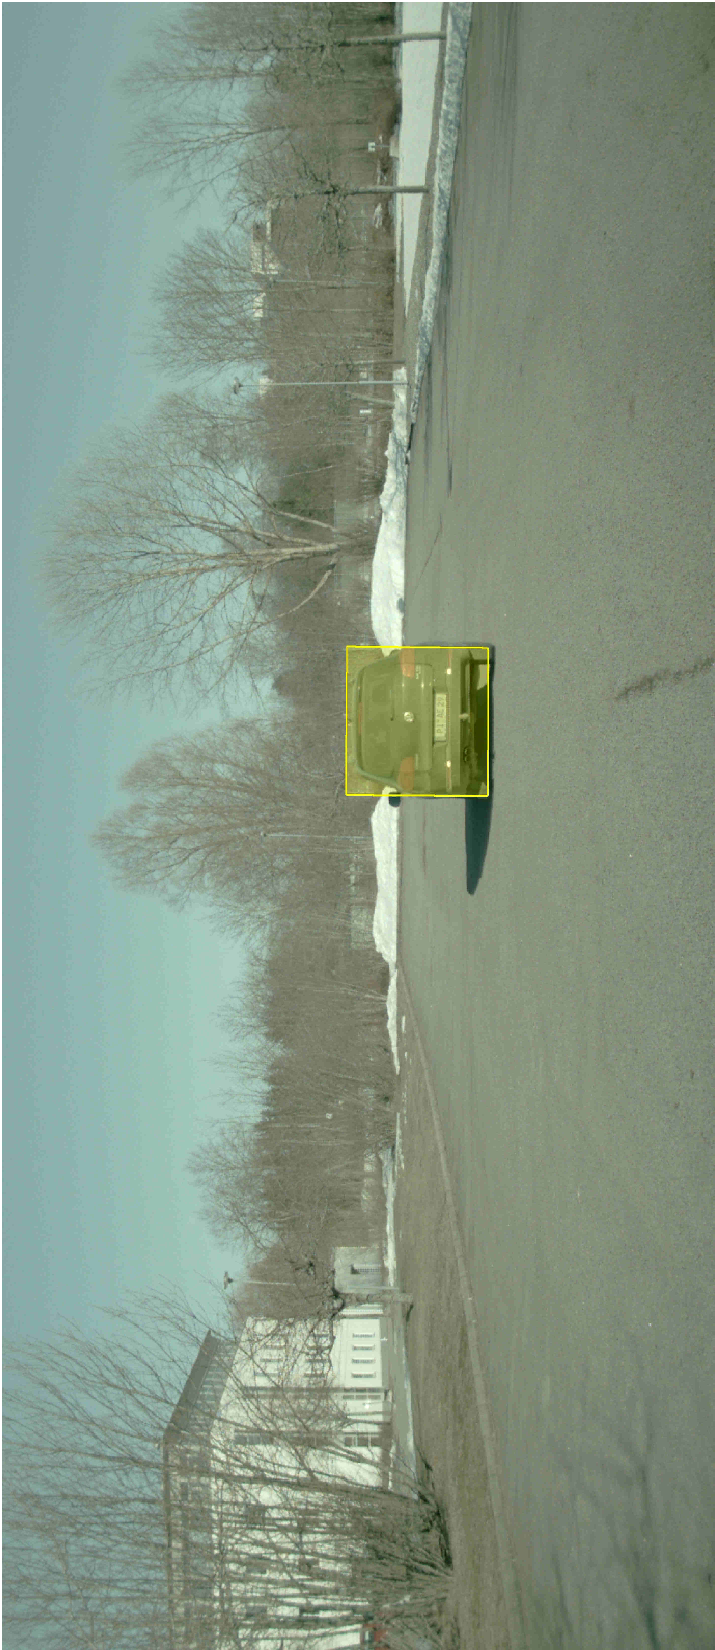
\includegraphics[angle=-90,origin=c,trim={0 0 15cm 0},width=0.9\textwidth]{roi_example}
	\caption{\label{fig:roiexample} An example of a vehicle that has been detected in a mono camera system using a classification appearance-based method. The vehicle has been marked by a box, referred to as the region of interest (\abbrROI).}
\end{figure}

\paragraph{Motion-based methods:}
Motion-based methods detect vehicles over a sequence of image frames.
Optical flow is one example of a method that can be used.
Optical flow is the motion of objects between frames, \ie how the pixels have moved from one frame to another.
The concept exists both as sparse optical flow, \ie the optical flow for a certain number of points in the image, and dense optical flow, \ie optical flow for all points in an image.

\subsection{Vehicle Tracking in Mono Camera Systems}
The goal of vehicle tracking is to predict and estimate \eg the position and velocity of the targets.
Many of the general object tracking aspects play an important role in vehicle tracking, \eg measurements, data association and \abbrMTT.
When tracking vehicles in a mono camera system, some alternatives are possible on how to select the states.
One can either track the vehicle in the image frame using image coordinates for position and velocity, or track in \spacedim{3} world coordinates and thus use meter and meter per second as units.
Since no depth information can be obtained from just a mono camera, some additional assumptions or other methods must be used if it is desired to track the target in \spacedim{3} world coordinates.

One of the main purposes of vehicle tracking is to maintain a state estimate of a vehicle even if it is not detected in a certain frame.
The tracking can \eg be performed with a filter of Kalman filter \cite{Sivaraman:2013} type.

\section{Related Research}
\label{sec:relatedresearch}
There exist several successful attempts of estimating the \spacedim{3} pose of objects using a mono camera system.
The problem of estimating the heading (including both the orientation and angular rate) of a vehicle can be seen as a special case of a full \spacedim{3} pose estimation problem.
A vehicle does not have the same degrees of freedom since it has limited rotational freedom.
\Figureref{fig:vehiclerotation} shows the rotation of interest, \ie the rotation around the axis which is perpendicular to the vehicle's ground plane.
Some different approaches found in the literature will be mentioned here.

\begin{figure}[!ht]
	\centering
	\begin{tikzpicture}
		[cube/.style={very thick,black}, wheel/.style={thick,black}]

		%draw the top and bottom of the cube
		\draw[cube] (0,0,0) -- (0,2,0) -- (2,2,0) -- (2,0,0) -- cycle;
		\draw[cube] (0,0,4) -- (0,2,4) -- (2,2,4) -- (2,0,4) -- cycle;

		%draw the edges of the cube
		\draw[cube] (0,0,0) -- (0,0,4);
		\draw[cube] (0,2,0) -- (0,2,4);
		\draw[cube] (2,0,0) -- (2,0,4);
		\draw[cube] (2,2,0) -- (2,2,4);

		\draw[wheel] (2,0,3) ellipse (0.2cm and 0.4cm);
		\draw[wheel] (0,0,3) ellipse (0.2cm and 0.4cm);
		\draw[wheel] (0,0,1) ellipse (0.2cm and 0.4cm);
		\draw[wheel] (2,0,1) ellipse (0.2cm and 0.4cm);

		%draw wheel axis
		\draw[cube, dashed] (0,0,3) -- (2,0,3);
		\draw[cube, dashed] (0,0,1) -- (2,0,1);

		\draw[cube, dashed] (1,0,3) node[circle,fill,inner sep=2pt] {} -- (1,4.5,3);
		%\draw[thick,dashed,red,->] (1,3,3) arc[x radius = 0.5cm, y radius = 0.75cm, start angle = 0, end angle = 180];
		\draw[very thick,red,->,>=stealth,rotate around={45:(1.5,3.5,3)}] (1.5,3.5,3) arc (0:300:0.8cm and 0.4cm);
		%\draw[thick,dashed,red,rotate around={-35:(1,3,3)}] (1,3,3) circle (0.5cm and 0.75cm);
	\end{tikzpicture}
	\caption{\label{fig:vehiclerotation} An illustration of which axis rotation that is of interest to estimate for a vehicle.}
\end{figure}

One straightforward way of estimating the \spacedim{3} pose of an object is to track a number of feature points over time and let an extended Kalman filter (\abbrEKF) estimate the rotation and translation parameters \cite{Hajimolahoseini:2014}.
By including the projection from \spacedim{3} to \spacedim{2}, the \abbrEKF estimates all necessary states directly.
No extra step to deal with the image projection is necessary.
The drawback is that the initial \spacedim{3} coordinates of the feature points must be known to a certain degree, which can be difficult to obtain from just a single image.
This method utilizes only image coordinates from the selected feature points as measurements.

In \cite{Blostein:2000}, another approach of estimating the \spacedim{3} pose is proposed.
Here, the \spacedim{3} trajectory and object structure are recovered from a sequence of images.
Especially, the optical flow for each selected feature point is utilized to improve the estimate instead of just using the image coordinates of feature points.
The usage of quaternions can be questioned, but might be good if the tracked object rotates in all three degrees of freedoms.
Using quaternions avoids the gimbal lock, which can occur when the pitch angle approaches 90 degrees \cite{Gustafsson:2012}.

Using the concept of homographies, \ie to estimate how planes have transformed between frames, is another concept, utilized in \cite{Gabb:2013}.
Here, the homography is estimated between frames in order to create a measurement of the angular rate of the target vehicle.
This method relies on having good correspondence between feature points in consecutive frames.
The Kanade-Lucas-Tomasi (\abbrKLT) feature tracker, \eg \cite{Szeliski:2011}, were used to track feature correspondences, between image frames.
The constructed measurement was used together with an \abbrEKF to obtain the state estimates.

In \cite{Mondragon:2010}, the homography concept is used in a somewhat similar manner.
Here, the yaw angle of an unmanned aerial vehicle (\abbrUAV) is estimated by calculating the homographies over time.
A helipad is placed on the ground as a reference plane onto which the homography is estimated.
Two flight tests were presented, and the resulting root-mean-square error (\abbrRMSE) of the yaw angle were $2.5^\circ$ and $4.9^\circ$, respectively.
A IMU was used as ground truth data.

\section{Coordinate Systems}
To describe tracking targets from a host, referring to the host as the ego vehicle in which the camera system is located, some terminology about different coordinate systems is necessary.
First, we have the difference between a world coordinate system  and an image coordinate system.
A world coordinate system is a coordinate system in \spacedim{3} representing how objects are positioned in the world.
An image coordinate system is the \spacedim{3} world coordinates projected onto a \spacedim{2} image plane.

\vspace{1em}

The image coordinate system is defined in \Figureref{fig:imagecoordsystem}.
It is used to \eg express measurements from a mono camera system.

Two world coordinate systems are defined and used in this thesis: the target's coordinate system and the host's coordinate system.
The states of the tracked target will be expressed in both the host's world coordinate system and the target's world coordinate system.
They are defined in \Figuresref{fig:hostcoordsystem} and \ref{fig:targetcoordsystem}, respectively.

\vspace{4em}

\begin{figure}[!ht]
	\centering
	\begin{tikzpicture}
		\node [draw,circle,fill,inner sep=1pt] (origin) at (-3,2) {};
		\draw (origin.center) -- (-3,-2) -- (3,-2) -- (3,2)  -- cycle;
		\draw[very thick,->] (origin) -- (-1,2) node[anchor=south] {$u$};
		\draw[very thick,->] (origin) -- (-3,0) node[anchor=east] {$v$};
	\end{tikzpicture}
	\caption{\label{fig:imagecoordsystem} The definition of the image coordinate system. The origin is located in the upper left corner.}
\end{figure}

\vfill

\begin{figure}[!ht]
    \centering
    \begin{tikzpicture}
    [cross/.style={path picture={
		\draw[black]
			(path picture bounding box.south east) -- (path picture bounding box.north west) (path picture bounding box.south west) -- (path picture bounding box.north east);
	}}]
		\node [draw,circle,cross,minimum width=0.1 cm](origo) at (2, 0.75) {};
		\node [draw,circle,inner sep=6pt] (wheela) at (-1.2,-1) {};
		\node [draw,circle,inner sep=6pt] (wheelb) at (1.2,-1) {};

		\draw (-2,-1) -- (wheela) -- (wheelb) -- (2,-1) -- (origo) -- (2,1) -- (-2,1) -- (-2,-1);
		\draw[thick] (-3,-1.3) -- (3,-1.3);
		\draw[->] (origo) node[anchor=south west] {$y$} -- (4, 0.75) node[anchor=west] {$x$};
		\draw[->] (origo) -- (2, 2.75) node[anchor=south] {$z$};

		\draw[->] (-1.5, 1.4) -- (1.5, 1.4) node[anchor=south east] {Traveling direction};
    \end{tikzpicture}
    \caption{\label{fig:hostcoordsystem} The definition of the host's coordinate system. The coordinate system is placed at the height of the mounted camera system with the origin placed at the principal point of the camera. The $x$-direction points in the same direction as the host itself, the $y$-direction points to the left when looking in the host's direction and the $z$-direction points upwards.}
\end{figure}

\begin{figure}[!ht]
    \centering
    \hspace*{2cm}
    \begin{tikzpicture}[scale=0.95, every node/.style={scale=0.95}]
		\node [draw,circle,inner sep=3pt] (origo) at (0,-1) {};
		\draw (-1.5,-2) rectangle (1.5,2);
		\draw[dashed] (-1.5,-1) -- (1.5,-1) node[pos=0.5,circle,fill,inner sep=1pt] {};
		\draw[->] (origo) node[anchor=north west] {$z$} -- (0,1) node[anchor=south] {$x$};
		\draw[->] (origo) -- (-2,-1) node[anchor=east] {$y$};
		\draw[->] (1.9,-1.5) -- (1.9,1.5) node[pos=0.5, anchor=west] {Traveling direction};
    \end{tikzpicture}
    \caption{\label{fig:targetcoordsystem} The definition of the target's coordinate system. The coordinate system is placed at the center of the rear axis of the target. The $x$-direction points in the same direction as the target itself, the $y$-direction  points to the left when looking in the target's direction and the $z$-direction points upwards.}
\end{figure}

\newpage

\section{The Pinhole Camera Model}
One basic camera model is the pinhole camera model \cite{Hartley:2004}.
It describes how a point in world coordinates projects onto the image coordinate system.
\Figureref{fig:pinholecameraex} illustrates how a point $(x, y, z)^T$ is mapped onto the image plane.
If the camera has the focal lengths $f_u$ and $f_v$, and by identifying similar triangles, the resulting mapping from \spacedim{3} to \spacedim{2} is
\begin{subequations}
\begin{equation}
    (x, y, z)^T \mapsto \left(f_u\frac{y}{x}, f_v\frac{z}{x}\right)^T,
\end{equation}
\ie
\begin{equation}
    (u, v)^T \mapsto \left(f_u\frac{y}{x}, f_v\frac{z}{x}\right)^T.
\end{equation}
\end{subequations}

\begin{figure}[!ht]
	\centering
	\begin{tikzpicture}
		[scale=0.9, every node/.style={scale=0.9},
		axis/.style={thick,black,->},
		 cross/.style={path picture={
			\draw[black]
			(path picture bounding box.south east) -- (path picture bounding box.north west) (path picture bounding box.south west) -- 			(path picture bounding box.north east);}}]
		\node [draw,circle,cross,minimum width=0.1 cm] (origin) at (0,0) {};
		\coordinate (xaxis) at (6,0);
		\coordinate (zaxis) at (0,3);

		% Coordinate axis
		\draw[axis] (origin) node[anchor=north east] {$y$} -- (xaxis) node[anchor=north] {$x$};
		\draw[axis] (origin) -- (zaxis) node[anchor=east] {$z$};

		% Image plane
		\draw[very thick] (2,-1) -- (2,4) node[anchor=south] {Image plane};

		% 3D coordinate
		\draw[] (origin) -- (6,3) node[anchor=west] {$(x,y,z)$} node[circle,fill,inner sep=1pt] {};
		
		% Focal axis
		\draw[->] (0,-0.25) -- (2,-0.25) node[pos=0.5,anchor=north] {$f_v$};

		% Projected size in image
		\draw[->] (2.25,0) -- (2.25, 1) node[pos=0.5,anchor=west] {$f_v \frac{z}{x}$};
	\end{tikzpicture}
	\caption{\label{fig:pinholecameraex} A world coordinate $(x, y, z)^T$ is projected onto the image plane. The figure shows the similar triangles for the projection in the $v$-direction.}
\end{figure}

\section{Homography}
\label{sec:homography}
The homography is a projective transformation.
The exact definition and more about projective transformations can be found in \eg \cite{Hartley:2004}, more precisely as Definitions 2.9 and 2.11, and Theorem 2.10.
Definition 2.11 from \cite{Hartley:2004} is of special interest, so it is recapitulated here and referred to as \Definitionref{def:projtrans}.

\begin{definition}[Projective transformation] \label{def:projtrans}
	A planar projective transformation is a linear transformation on homogeneous \spacedim{3} vectors represented by a nonsingular $3 \times 3$ matrix:
	\begin{equation}
		\begin{pmatrix} x^\prime_1 \\ x^\prime_2 \\ x^\prime_3 \end{pmatrix}
		=
		\begin{pmatrix}
			h_{11} & h_{12} & h_{13} \\
			h_{21} & h_{22} & h_{23} \\
			h_{31} & h_{32} & h_{33}
		\end{pmatrix}
		\begin{pmatrix} x_1 \\ x_2 \\ x_3 \end{pmatrix},
	\end{equation}
	or in short, $\bm{x}^\prime = \bm{H} \bm{x}$.
\end{definition}
%
As described in \cite{Nordberg:2015}, any nonzero scalar multiplied into $\bm{H}$ is also a representative of the same homography.
The projective transformation can therefore be formulated as
%
\begin{subequations}
\begin{equation}
	\label{eq:homography}
	\bm{x}^\prime \sim \bm{H} \bm{x},
\end{equation}
%
or by using an equality sign,
%
\begin{equation}
	\label{eq:homographyequality}
	\gamma \bm{x}^\prime = \bm{H} \bm{x},
\end{equation}
\end{subequations}
%
for some nonzero scalar $\gamma$.
One example of how a projective transformation can be used, mentioned in \cite{Hartley:2004}, is mapping between planes. 
This is the idea used in \cite{Gabb:2013} to estimate the angular rate of vehicles and in \cite{Mondragon:2010} to estimate the yaw angle of a \abbrUAV.

The problem of estimating how a plane in \spacedim{3}, given a set of image coordinates $\bm{x}_i \in \mathbb{P}^2$ and a corresponding set of image coordinates $\bm{x}^\prime_i \in \mathbb{P}^2$, has moved (translated and rotated) between two frames is equivalent to finding the homography $\bm{H}$ for the two correspondence set of homogeneous image coordinates $\bm{x} = (u_i, v_i, 1)^T$ and $\bm{x}^\prime = (u^\prime_i, v^\prime_i, 1)^T$.
The interpretation of corresponding points is a point before and the same point after the homography transformation.
There exist several methods for finding the homography from the corresponding points.

\subsection{Direct Linear Transform}
The homography matrix, $\bm{H}$, can be estimated given a set of $N$ image coordinates, $\bm{x}_i = (u_i, v_i, 1)^T$, and the correspondence set of $N$ image coordinates, $\bm{x}^\prime_i = (u^\prime_i, v^\prime_i, 1)^T$, in another frame.

By rewriting \eqref{eq:homographyequality}, and by substituting the third row, $\gamma_i = h_{31}u_i + h_{32}v_i + h_{33}$, into the other two rows, a resulting linear equation system on the form
%
\begin{equation}
	\label{eq:geoerrorhomography}
	\bm{A} \bm{h} = \bm{0}
\end{equation}

\vspace{1em}

is obtained and is referred to as a direct linear transformation (\abbrDLT), \eg \cite{Hartley:2004} and \cite{Nordberg:2015}, where $\bm{A}$ is a $2 N \times 9$ matrix and $\bm{h}$ is a $9 \times 1$ vector,
%
\begin{equation}
	\bm{A} =
	\begin{pmatrix}
		u_1 & 0 & -u_1 u_1^\prime & v_1 & 0 & - v_1 u_1^\prime & 1 & 0 & -u_1^\prime \\
		0 & u_1 & -u_1 v_1^\prime & 0 & v_1 & - v_1 v_1^\prime & 0 & 1 & -v_1^\prime \\
		\vdots & \vdots & \vdots & \vdots & \vdots & \vdots & \vdots & \vdots & \vdots \\
		u_N & 0 & -u_N u_N^\prime & v_N & 0 & - v_N u_N^\prime & 1 & 0 & -u_N^\prime \\
		0 & u_N & -u_N v_N^\prime & 0 & v_N & - v_N v_N^\prime & 0 & 1 & -v_N^\prime
	\end{pmatrix}
	,
	\quad
	\bm{h} =
	\begin{pmatrix}
		h_{11} \\
		h_{21} \\
		h_{31} \\
		h_{12} \\
		h_{22} \\
		h_{32} \\
		h_{13} \\
		h_{23} \\
		h_{33} \\
	\end{pmatrix}
	.
\end{equation}
%
Viewing \eqref{eq:geoerrorhomography} as a least squares problem, turns \eqref{eq:geoerrorhomography} into the optimization problem
%
\begin{equation}
	\min_{\bm{h}} \sum_i
	\left( u^\prime_i - \frac{h_{11}u_i + h_{12}v_i + h_{13}}{h_{31}u_i + h_{32}v_i + h_{33}} \right)^2 +
	\left( v^\prime_i - \frac{h_{21}u_i + h_{22}v_i + h_{23}}{h_{31}u_i + h_{32}v_i + h_{33}} \right)^2.
\end{equation}

\subsection{Random Sample Consensus}
\label{sec:ransac}
If the data contains outliers, the \abbrDLT solution generally results in a bad estimate.
Since all data points have equal weights, outliers, \ie points that do not fit the estimated model, can have significant impact on the estimation result.
Random sample consensus (\abbrRANSAC), \eg \cite{Hartley:2004} and \cite{Nordberg:2015}, is one method which can improve the result if the data set contains outliers.
The method contains some tuning parameters selected by the user.
Some notable notations used in the algorithm are:

\begin{description}[align=left,labelwidth=3cm,noitemsep]
	\item [Trial set $T$] A random subset of the total data set.
	\item [Consensus set $\bm{C}$] All data points satisfying the homography estimated from $T$.
	\item [Threshold $t$] Determines if a corresponding point pair belongs to $\bm{C}$ or not.
	\item [Number of trials $r$] The number of times a trial set $T$ is selected.
\end{description}

The complete algorithm with all details can be found in \cite{Nordberg:2015}.
Here, a brief overview of the algorithm is provided in \Algorithmref{algo:ransach}.

\begin{algorithm}[!ht]
	\caption{\label{algo:ransach} A \abbrRANSAC algorithm for estimating the homography}
	\begin{algorithmic}
		\State \textbf{input} data set $D$, threshold $t$, number of trials $r$
		\State Initialize $\bm{H}_\text{est} = \emptyset$ and $\bm{C}_\text{est} = \emptyset$
		\While {$i = \{1,\dots,r\}$}
			\State Pick a random subset $T$ with 4 pairs of corresponding points from $D$
			\State Determine $\bm{H}$ from $T$ using the \abbrDLT method
			\State Initialize $\bm{C} = \emptyset$
			\ForAll {point pair $\{\bm{x}^\prime, \bm{x}\}$ in the data sets $D$}
				\State Compute an error $\epsilon$, measuring how well $\{\bm{x}^\prime, \bm{x}\}$ fits $\bm{H}$
				\If {$\epsilon < t$}
					\State Add $\{\bm{x}^\prime, \bm{x}\}$ to $\bm{C}$
				\EndIf
			\EndFor
			\If {size of $\bm{C}$ is larger than size of $\bm{C}_\text{est}$}
				\State Set $\bm{H}_\text{est} = \bm{H}$ and $\bm{C}_\text{est} = \bm{C}$
			\EndIf
		\EndWhile
		\State \Return $\bm{H}_\text{est}$ and $\bm{C}_\text{est}$
	\end{algorithmic}
\end{algorithm}

\clearpage

\section{Feature Points}
In order to get the corresponding image coordinates, mentioned in \Sectionref{sec:homography}, and the optical flow, mentioned in \Sectionref{sec:objectdetection}, a selection of certain points from the image, referred to as feature points, has to be done.
An example of detected feature points in an image can be seen in \Figureref{fig:featurepointexample}.
There exist mainly three different steps, where the last step can be performed in two ways, when detecting feature points and finding the correspondence between images \cite{Szeliski:2011}.
They are:

\begin{description}[align=left,labelwidth=3cm]
	\item [Feature detection] Find and extract image points that are easily recognisable and distinguishable from its surroundings. Typically, this means points that have a large image gradient.
	\item [Feature description] A descriptor is an alternative representation of the image point. Its purpose is to be a robust description of the feature point and its surrounding region. Examples of descriptors are: Scale-invariant feature transform (SIFT) and gradient location and orientation histogram (GLOH) \cite{Szeliski:2011}.
	\item [Feature matching] Feature points are separately extracted from two consecutive images and then the descriptors are compared in order to matched points between the two images.
	\item [Feature tracking] Instead of matching extracted feature points between two images, one can in the second frame search for the feature points detected in the first frame, \ie track the feature points. The \abbrKLT tracker is a popular feature point tracker.
\end{description}

\begin{figure}[!ht]
	\centering
	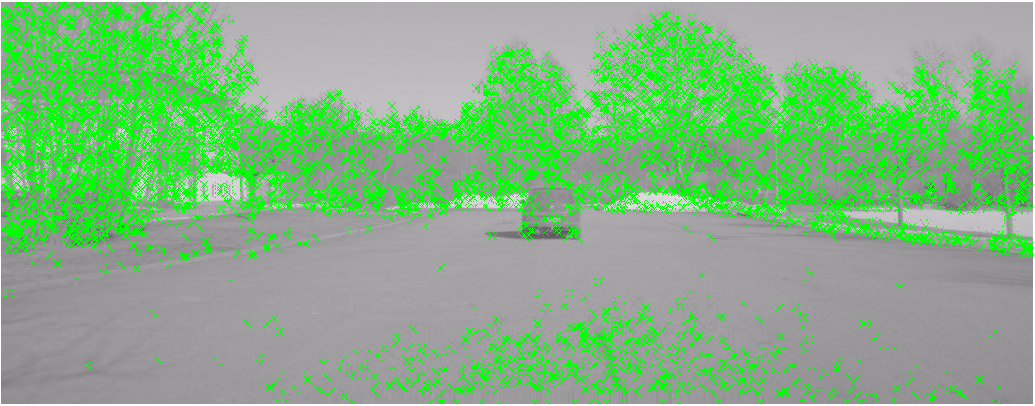
\includegraphics[width=0.9\textwidth]{155532_harris_features}
	\caption{\label{fig:featurepointexample} An example of an image with detected feature points marked as green crosses. Here, the Harris–Stephens corner detection algorithm \cite{Harris:1988} was used to detect interesting points.}
\end{figure}

\newpage

\section{Extended Kalman Filtering}
Kalman filtering \cite{Gustafsson:2012} is one filtering method used to track a target.
If the target is moving according to some motion model, $\bm{f}(\bm{x}_k,\bm{u}_k,\bm{v}_k)$, and measurements are generated according to some measurement model, $\bm{h}(\bm{x}_k,\bm{u}_k,\bm{e}_k)$, the system is described by
\begin{align}
\begin{split}
	\bm{x}_{k+1} &= \bm{f}(\bm{x}_k,\bm{u}_k,\bm{v}_k), \\
	\bm{y}_k &= \bm{h}(\bm{x}_k,\bm{u}_k,\bm{e}_k).
\end{split}
\end{align}
Here, $\bm{x}_k$ is the state of the target, $\bm{u}_k$ is an input or control signal to the system, $\bm{v}_k$ is the process noise and $\bm{e}_k$ is the measurement noise.
The process and measurement noise are assumed to be Gaussian with zero mean and covariance matrices denoted $\bm{Q}$ and $\bm{R}$, respectively.
The motion and measurement models used in this thesis are nonlinear, thus the \abbrEKF can be applied.
The algorithm to perform \abbrEKF filtering can be found in \cite{Gustafsson:2012} and is recapitulated in \Algorithmref{algo:ekf}.
In the algorithm outline, the input signal $\bm{u}_k$ has been omitted.

\begin{algorithm}
	\caption{\label{algo:ekf} Extended Kalman filtering algorithm}
	Given some initial conditions, $\hat{\bm{x}}_{1|0}$ and $\bm{P}_{1|0}$, the \abbrEKF solves the filtering problem by a, two step, recursion algorithm. \\ \\
	\begin{subequations}
	Measurement update:
	\begin{align}
		\bm{S}_k &= \bm{R}_k + \bm{h}^\prime(\hat{\bm{x}}_ {k|k-1}) \bm{P}_{k|k-1} (\bm{h}^\prime(\hat{\bm{x}}_ {k|k-1}))^T \\
		\bm{K}_k &= \bm{P}_{k|k-1} (\bm{h}^\prime(\hat{\bm{x}}_ {k|k-1}))^T \bm{S}_k^{-1} \\
		\bm{\epsilon}_k &= \bm{y}_k - \bm{h}(\hat{\bm{x}}_{k|k-1}) \\
		\hat{\bm{x}}_{k|k} &= \hat{\bm{x}}_{k|k-1} + \bm{K}_k \bm{\epsilon}_k \\
		\bm{P}_{k|k} &= \bm{P}_{k|k-1} - \bm{K}_k \bm{h}^\prime(\hat{\bm{x}}_{k|k-1}) \bm{P}_{k|k-1}
	\end{align}
	\\
	Time update:
	\begin{align}
		\hat{\bm{x}}_{k+1|k} &= \bm{f}(\hat{\bm{x}}_{k|k}) \\
		\bm{P}_{k+1|k} &= \bm{Q}_k + \bm{f}^\prime(\hat{\bm{x}}_{k|k}) \bm{P}_{k|k} (\bm{f}^\prime(\hat{\bm{x}}_{k|k}))^T
	\end{align}
	\end{subequations}
\end{algorithm}

Here, $\bm{f}^\prime(\hat{\bm{x}}_k)$ and $\bm{h}^\prime(\hat{\bm{x}}_k)$ are the Jacobians of $\bm{f}(\hat{\bm{x}}_k)$ and $\bm{h}(\hat{\bm{x}}_k)$, respectively.
The matrices $\bm{R}_k$ and $\bm{Q}_k$ are the covariance matrices of $\bm{e}_k$ and $\bm{v}_k$, respectively.
The algorithm is based on the first order moment Taylor expansion.

\section{Observability Analysis}
\label{sec:obsanalysis}
To be able to estimate the state $\bm{x}_k$, from the available measurements, the system must be observable.
For a system on linear state-space form,
\begin{align}
\label{eq:linearss}
\begin{split}
	\bm{x}_{k+1} &= \bm{A}_k \bm{x}_k + \bm{B}_k \bm{u}_k, \\
	\bm{y}_k &= \bm{C}_k \bm{x}_k + \bm{D}_k \bm{u}_k,
\end{split}
\end{align}
the observability can be determined using the observability Gramian \cite{Rugh:1996}.
Recalling the definition of observability from \cite{Rugh:1996}, which gives \Definitionref{def:observability}.

\begin{definition}[Observability] \label{def:observability}
	The linear state-space model \eqref{eq:linearss} is observable in the interval $[t_0, t_N]$ if any initial state $\bm{x}_0$ is uniquely determined by the corresponding zero-input response $\bm{y}_k$ for $k=t_0,\dots,t_N-1$.
\end{definition}

The condition for having an observable linear state equation is given by \Theoremref{th:observability} from \cite{Rugh:1996}.
%
\begin{theorem}
\label{th:observability}
	The linear state equation \eqref{eq:linearss} is observable on $[t_0, t_N]$ if and only if the $n \times n$ matrix
	\begin{equation}
	\label{eq:observabilitytheorem}
		\bm{M}(t_0,t_N) = \sum_{j=t_0}^{t_N-1} \bm{\Phi}^T(j,t_0)\bm{C}^T_j\bm{C}_j\bm{\Phi}(j,t_0)
	\end{equation}
	is invertible.
\end{theorem}
%
Here, the matrix $\bm{M}$ is the observability Gramian and $\bm{\Phi}$ is the transition matrix, which is, for $k \ge j$, given by
%
\begin{equation}
	\bm{\Phi}(k,j) =
		\begin{cases}
			\bm{A}_{k-1} \bm{A}_{k-2} \cdots \bm{A}_j & \text{if } k \ge j+1, \\
			\bm{I} & \text{if } k = j.
		\end{cases}
\end{equation}
%
In the case of a nonlinear state-space model,
%
\begin{align}
\label{eq:nlss}
\begin{split}
	\bm{x}_{k+1} &= \bm{f}(\bm{x}_k), \\
	\bm{y}_k &= \bm{h}(\bm{x}_k),
\end{split}
\end{align}
%
where the control signal $\bm{u}_k$ has been omitted, the state-space model first has to be linearized.
By linearizing using a Taylor expansion and retaining only the first order terms, the resulting linearized state-space model is
%
\begin{equation}
\begin{split}
	\bar{\bm{x}}_{k+1} = \bm{f}^\prime(\bm{\tilde{\bm{x}}_k}) \bar{\bm{x}}_k, \\
	\bar{\bm{y}}_{k} = \bm{h}^\prime(\bm{\tilde{\bm{x}}_k}) \bar{\bm{x}}_k,
\end{split}
\end{equation}
%
where $\bm{x}_k = \tilde{\bm{x}}_k + \bar{\bm{x}}_k$ and $\tilde{\bm{x}}_k$ is the point around which the Taylor expansion took place, the matrix $\bm{f}^\prime(\bm{\tilde{\bm{x}}_k})$ is the Jacobian of $\bm{f}(\bm{x}_k)$ and $\bm{h}^\prime(\bm{\tilde{\bm{x}}_k})$ is the Jacobian of $\bm{h}(\bm{x}_k)$, respectively.
The model now fits into the structure of \Definitionref{def:observability} and \Theoremref{th:observability}.

\chapter{Filter Construction and Methodology}
\label{cha:method}

In this chapter, a method is proposed to solve the heading estimation problem.
The main idea is to compute how the front (or the back) of the target has moved between two consecutive frames, \ie estimate the homography.
From the homography, the relative rotation, \ie the angular rate, can be extracted and used as a measurement.
By combining the new angular rate measurement and \abbrROI measurements from machine learning algorithms, together with a suitable vehicle and motion model, the system can be implemented in \matlab and evaluated against results from a stereo camera system.

The chapter describes the motion model used to predict the motion of the target, the measurement model for both the image detections and angular rate and how all measurements are fused together in an \abbrEKF.
It also describes how to, if they were accessible, incorporate measurements of the target vehicle's corners into the model.

\section{Vehicle Motion Model}
By taking inspiration from a standard constant velocity model \eg mentioned in \cite{Gustafsson:2012}, a motion model is constructed for target vehicles.
In discretized form, under the assumption that the target vehicle moves with constant velocity during a sample interval $T$, the motion model is described by
%
\begin{subequations}
\label{eq:motionmodel}
\begin{align}
    \begin{pmatrix}
        x_{k+1} \\
        y_{k+1}
    \end{pmatrix}
    &=
    \begin{pmatrix}
        x_k \\
        y_k
    \end{pmatrix}
    +
    \rotmat\left(\psi_k + \omega_k T\right)
    \begin{pmatrix}
        v_k T \\
        0
    \end{pmatrix}
    +
    \begin{pmatrix}
    	v^x \\
    	v^y
    \end{pmatrix},
    \label{eq:motionmodel-1}
    \\
    z_{k+1} &= z_k + v^z,
    \label{eq:motionmodel-2}
    \\
    v_{k+1} &= v_k + v^v,
    \label{eq:motionmodel-3}
    \\
    \psi_{k+1} &= \psi_k + \omega_k T + v^\psi,
    \label{eq:motionmodel-4}
    \\
    \omega_{k+1} &= \omega_k + v^\omega,
    \label{eq:motionmodel-5}
\end{align}
\end{subequations}
%
where $\rotmat$ is the \spacedim{2} rotation matrix, defined as
\begin{equation*}
	\rotmat(\theta) =
	\begin{pmatrix}
	\cos\theta & -\sin\theta \\
	\sin\theta & \cos\theta
	\end{pmatrix},
\end{equation*}
and $v^x, v^y, v^z, v^v, v^\psi$ and $v^\omega$ are the process noise.

The notation used in \eqref{eq:motionmodel} is defined in \Tableref{tab:motionmodel} and \Figureref{fig:motionmodel} illustrates how the notions are related to the target vehicle.
One thing to note is that the tracking is performed relative to the host, \ie the position and orientation are expressed in the host's world coordinate system.
Compared to the constant velocity model in \cite{Gustafsson:2012}, some differences can be noted.
The $z$-position is assumed to be constant for natural reasons.
The angular rate $\omega$ is also assumed to be constant and the yaw angle $\psi$ is updated accordingly.

\begin{figure}[!ht]
	\centering
	\begin{tikzpicture}[scale=0.85, every node/.style={scale=0.85}]
        % --- Draw rectangle car ---
        \draw (0,0) -- (3,1) -- (1.5,5.5) -- (-1.5,4.5) -- cycle;
        \draw[dashed] (-0.5,1.5) -- (2.5,2.5) node[pos=0.6, anchor=north] {$(x,y,z)$};
        \draw[->] (1,2) node[circle,fill,inner sep=1pt] {} -- (0.3,4) node[anchor=south] {$v$};
        \draw[dotted] (1,2) -- (1,4);
        \draw[<-] (0.65,3) .. controls (0.8,3.1) .. (1,3.1) node[pos=0.5, anchor=south] {\hspace{0.3cm}$\psi, \omega$};
        % ---
    \end{tikzpicture}
    \caption{\label{fig:motionmodel} The notation in the motion model related to the target vehicle.}
\end{figure}

If the host is moving while tracking the target, at each sample, \ie frame, the state of the target must be compensated with respect to the host's ego motion.
It has been omitted from \eqref{eq:motionmodel} in order to simplify the expressions and as mentioned in \Chapterref{cha:intro}, the thesis deals only with host cars with no ego motion.
A generalized formulation of the compensation is
%
\begin{equation}
	\bm{x}_{k+1} = \bm{f}_{\text{Motion}}\left( \bm{f}_{\text{Ego}}(\bm{x}_k) \right),
\end{equation}
%
where $\bm{f}_{\text{Ego}}$ is the function which compensates for the host's ego motion and $\bm{f}_{\text{Motion}}$ is the motion model in \eqref{eq:motionmodel}.
%
\begin{table}[!ht]
\centering
\caption{\label{tab:motionmodel} The variables in the motion model for the target.}
    \begin{tabular}{|c|p{9cm}|}
    \hline
    \textbf{Notation} & \textbf{Definition} \\
    \hline
    \rule{0pt}{1.1em}
    $\bm{x}$ & The target's state vector, \ie $\bm{x} = \left(x, y, z, v, \psi, \omega \right)^T$. \\
    \hline
    $x$ & The target's position in the $x$-direction of the host's coordinate system. \\
    \hline
    $y$ & The target's position in the $y$-direction of the host's coordinate system. \\
    \hline
    $z$ & The target's position in the $z$-direction of the host's coordinate system. \\
    \hline
    $v$ & The velocity of the target in the $x$-direction of the target's coordinate system. \\
    \hline
    $\psi$ & The yaw angle of the target compared to the host. \\
    \hline
    $\omega$ & The yaw rate of the target. \\
    \hline
    \end{tabular}
\end{table}

\section{Measurement Vehicle Model}
In order to estimate the orientation and angular rate, \ie the heading of a target, a measurement model must be constructed.
In \Figureref{fig:vehiclemodel}, the target vehicle is modelled as a rectangle.
The notation used in \Figureref{fig:vehiclemodel} is further described in \Tableref{tab:vehiclemodel}.
Since no direct distance measurement can be obtained, two assumptions about the width and length of the target must be used.

\begin{figure}[!ht]
    \centering
    \hspace{2cm}
    \begin{tikzpicture}[scale=1.2, every node/.style={scale=1.2}]
        % --- Draw rectangle car ---
        \draw (0,0) -- (3,1) -- (1.5,5.5) -- (-1.5,4.5) -- cycle;
        \draw[dashed] (-0.5,1.5) -- (2.5,2.5) node[pos=0.6, anchor=north] {$(x,y,z)$};
        \draw[->] (1,2) node[circle,fill,inner sep=1pt] {} -- (0.3,4) node[anchor=south] {$v$};
        \draw[dotted] (1,2) -- (1,4);
        \draw[<-] (0.65,3) .. controls (0.8,3.1) .. (1,3.1) node[pos=0.5, anchor=south] {$\psi$};
        % ---

        % --- Draw lines for length and width ---
        \draw[<->] (-0.25,-0.1) -- (-0.75,1.4) node[pos=0.5, anchor=east] {$\alpha l$};
        \draw[<->] (-0.75,-0.3) -- (-2.25,4.2) node[pos=0.5, anchor=east] {$l$};
        \draw[<->] (-1.6,4.8) -- (1.4,5.8) node[pos=0.5, anchor=south] {$w$};
        % ---

        % --- Host coordinate system ---
        \node[draw,circle,inner sep=2pt] (hostorigin) at (4,-0.5) {};
        \draw[thick, ->] (hostorigin) node[anchor=north west] {$z_\text{Host}$} -- (4,1) node[anchor=west] {$x_\text{Host}$};
        \draw[thick, ->] (hostorigin) node[circle,fill,inner sep=0.5pt] {} -- (2.5,-0.5) node[anchor=north east] {$y_\text{Host}$};
    \end{tikzpicture}
    \caption{\label{fig:vehiclemodel} The model of a target vehicle. The direction of the $x$-axis of the host's coordinate system coincides with the target's $x$-axis when the yaw angle $\psi$ is zero.}
\end{figure}

\begin{table}[!ht]
\centering
\caption{\label{tab:vehiclemodel} Notations used for describing the target vehicle.}
    \begin{tabular}{|c|p{9cm}|}
    \hline
    \textbf{Notation} & \textbf{Description} \\
    \hline
    $(x,y,z)$ & World coordinates of the target's position in the host's coordinate system. \\
    \hline
    $v$ & The velocity of the target, \ie the target's absolute velocity. \\
    \hline
    $\psi$ & Yaw angle of the target compared to the host. \\
    \hline
    $w$ & Assumed width of the target. \\
    \hline
    $l$ & Assumed length of the target. \\
    \hline
    $\alpha$ & Ratio describing the length of the car behind the rear axis. \\
    \hline
    \end{tabular}
\end{table}

By using the detection methods described in \Sectionref{sec:objectdetection}, image measurement models can be derived.

\newpage

\subsection{ROI Horizontal Center Position Measurement}

First, we have the measurement of the horizontal center position of the \abbrROI.
In \Figureref{fig:measurementmodelhcp}, a geometric view of the measurement is presented.
The observation is the middle of the back, or the front, of the target.
By utilizing the properties of the pinhole camera model, the measurement equation is
%
\begin{equation}
\begin{split}
    p_{\text{HCP, back}} &= -f_u \frac{y + (0,1,0) \rotmat(\psi) (- \alpha l,0,0)^T}{x + (1,0,0) \rotmat(\psi) (- \alpha l,0,0)^T} + e_{\text{HCP, back}}\\
    &= -f_u \frac{y - \alpha l \sin(\psi)}{x - \alpha l \cos(\psi)} + e_{\text{HCP, back}},
\end{split}
\end{equation}
%
where $e_{\text{HCP, back}}$ is the measurement noise and $\rotmat$ is the \spacedim{3} rotation matrix defined as
\begin{equation*}
	\rotmat(\theta) =
	\begin{pmatrix}
		\cos\theta & -\sin\theta & 0 \\
		\sin\theta & \cos\theta & 0 \\
		0 & 0 & 1
	\end{pmatrix}.
\end{equation*}
The measurement is the the number of pixels offset for the horizontal center position, compared to the center of the image in the $u$-direction.
This is illustrated in \Figureref{fig:roihcp}.
If instead the front of the target is observed, the factor $\alpha$ is changed to $\alpha-1$ (the point $((1-\alpha)l,0,0)^T$ is observed instead) and the resulting measurement equation is
%
\begin{equation}
    p_{\text{HCP, front}} = -f_u \frac{y - (\alpha - 1) l \sin(\psi)}{x - (\alpha - 1) l \cos(\psi)} + e_{\text{HCP, front}},
\end{equation}
%
where $e_{\text{HCP, front}}$ is the measurement noise.

% ROI Horizontal Center Position
\begin{figure}[!ht]
    \centering
    \begin{tikzpicture}[scale=0.85, every node/.style={scale=0.85}]
        % --- Draw rectangle car ---
        \draw (0,0) -- (3,1) -- (1.5,5.5) -- (-1.5,4.5) -- cycle;
        \draw[dashed] (-0.5,1.5) -- (2.5,2.5);
        \draw[->] (1,2) node[circle,fill,inner sep=1pt] {} -- (0.3,4) node[anchor=south] {$v$};
        \draw[dotted] (1,2) -- (1,4);
        \draw[<-] (0.65,3) .. controls (0.8,3.1) .. (1,3.1) node[pos=0.5, anchor=south] {$\psi$};
        % ---

        % --- Draw lines for length and width ---
        \draw[<->] (-0.25,-0.1) -- (-0.75,1.4) node[pos=0.5, anchor=east] {$\alpha l$};
        \draw[<->] (-0.75,-0.3) -- (-2.25,4.2) node[pos=0.5, anchor=east] {$l$};
        \draw[<->] (-1.6,4.8) -- (1.4,5.8) node[pos=0.5, anchor=south] {$w$};
        % ---

        % --- Draw image plane and associated lines---
        \coordinate (camOrigo) at (5.5, -4.5);
        \draw[very thick] (-1,-3) node[anchor=east] {Image plane} -- (8,-3);
        \draw[->] (6,-4.5) -- (6,-3) node[pos=0.5, anchor=west] {$f_u$};
        \draw[->] (6.5,-4.5) -- (6.5,2) node[pos=0.5, anchor=west] {$x$};
        \draw[->] (5.5,2.5) -- (1,2.5) node[pos=0.4, anchor=south] {$y$};
        \draw (camOrigo) node[circle,fill,inner sep=2pt] {} -- (5.5,2) -- (1,2) -- (1.5,0.5) node[circle,fill,inner sep=1pt] {} -- cycle;
        \draw (1.5,0.5) -- (5.5,0.5);
        \draw[->] (5.5,-2.6) -- (4.3,-2.6) node[pos=0.5, anchor=south] {$-p_{HCP}$};
        \draw (4.3,-2.5) -- (4.3,-3.2);
        % ---
    \end{tikzpicture}
    \caption{\label{fig:measurementmodelhcp} The measurement model for the \abbrROI horizontal center position when observing the back of the target.}
\end{figure}

\begin{figure}[!ht]
	\centering
	\begin{tikzpicture}
		\node[] at (0,0) {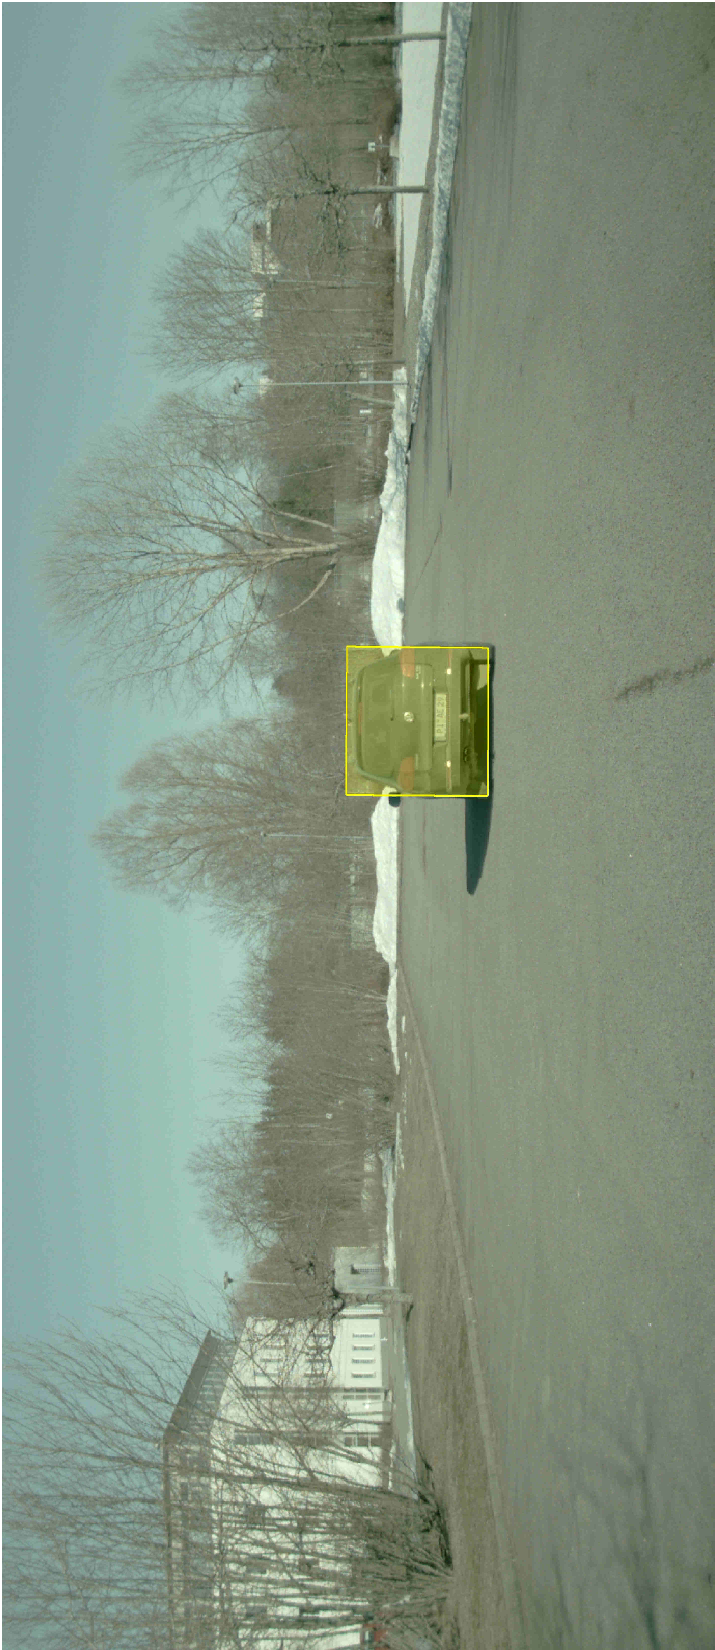
\includegraphics[angle=-90,origin=c,trim={0 0 15cm 0},width=0.85\textwidth]{roi_example}};
		\draw[red, very thick, |->] (0,-0.8) -- (0.7,-0.8) node[anchor=north] {$p_\text{HCP}$};
	\end{tikzpicture}
	\caption{\label{fig:roihcp} The \abbrROI horizontal center position measurement from real-world data.}
\end{figure}

\subsection{ROI Width Measurement}
The width of the \abbrROI is another image measurement model.
It is described in \Figureref{fig:measurementmodelwidth} and \Figureref{fig:roiwidth}.
By taking the difference between $i_1$ and $i_2$, the measurement equation becomes
%
\begin{equation}
\begin{split}
    p_{\text{Width, back}} = &i_1 - i_2 \\
    = &f_u \frac{y + (0,1,0) \rotmat(\psi) (- \alpha l,w/2,0)^T}{x + (1,0,0) \rotmat(\psi) (- \alpha l,w/2,0)^T} \\
    &- f_u \frac{y + (0,1,0) \rotmat(\psi) (- \alpha l,-w/2,0)^T}{x + (1,0,0) \rotmat(\psi) (- \alpha l,-w/2,0)^T} + e_ {\text{Width, back}} \\
    = &f_u \frac{y - \alpha l \sin(\psi) + w \cos(\psi) / 2}{x - \alpha l \cos(\psi) - w \sin(\psi) / 2} \\
    &- f_u \frac{y - \alpha l \sin(\psi) - w \cos(\psi) / 2}{x - \alpha l \cos(\psi) + w \sin(\psi) / 2} + e_ {\text{Width, back}} \\
    = &f_u \frac{(y - \alpha l \sin(\psi) + w \cos(\psi) / 2)(x - \alpha l \cos(\psi) + w \sin(\psi) / 2)}{(x - \alpha l \cos(\psi))^2 - w^2 \sin^2(\psi) / 4} \\
    &- f_u\frac{(y - \alpha l \sin(\psi) - w \cos(\psi) / 2)(x - \alpha l \cos(\psi) - w \sin(\psi) / 2)}{(x -  \alpha l \cos(\psi))^2 - w^2 \sin^2(\psi) / 4} \\
    &+ e_ {\text{Width, back}} \\
    = &-f_u \frac{\alpha l w - y \sin(\psi) w - x \cos(\psi) w}{(x - \alpha l \cos(\psi))^2 - w^2 \sin^2(\psi) / 4} + e_ {\text{Width, back}},
\end{split}
\end{equation}
%
where $e_ {\text{Width, back}}$ is the measurement noise.
If instead the front is observed, the factor $\alpha$ becomes $\alpha - 1$ and the order of the observed points is interchanged yielding the equation
%
\begin{equation}
\begin{split}
    p_{\text{Width, front}} = &i_1 - i_2 \\
    = &f_u \frac{y + (0,1,0) \rotmat(\psi) ((1-\alpha)l,-w/2,0)^T}{x + (1,0,0) \rotmat(\psi) ((1-\alpha)l,-w/2,0)^T} \\
    &- f_u\frac{y + (0,1,0) \rotmat(\psi) ((1-\alpha)l,w/2,0)^T}{x + (1,0,0) \rotmat(\psi) ((1-\alpha)l,w/2,0)^T} + e_ {\text{Width, front}} \\
    = &f_u \frac{(\alpha-1) l w - y \sin(\psi) w - x \cos(\psi) w}{(x - (\alpha-1) l \cos(\psi))^2 - w^2 \sin^2(\psi) / 4} + e_ {\text{Width, front}},
\end{split}
\end{equation}
%
where $e_{\text{Width, front}}$ is the measurement noise.

% ROI Width
\begin{figure}[!ht]
    \centering
    \begin{tikzpicture}
        % --- Draw rectangle car ---
        \draw (0,0) node[circle,fill,inner sep=1pt] {} -- (3,1) node[circle,fill,inner sep=1pt] {} -- (1.5,5.5) -- (-1.5,4.5) -- cycle;
        \draw[dashed] (-0.5,1.5) -- (2.5,2.5);
        \draw[->] (1,2) node[circle,fill,inner sep=1pt] {} -- (0.3,4) node[anchor=south] {$v$};
        \draw[dotted] (1,2) -- (1,4);
        \draw[<-] (0.65,3) .. controls (0.8,3.1) .. (1,3.1) node[pos=0.5, anchor=south] {$\psi$};
        % ---

        % --- Draw lines for length and width ---
        \draw[<->] (-0.25,-0.1) -- (-0.75,1.4) node[pos=0.5, anchor=east] {$\alpha l$};
        \draw[<->] (-0.75,-0.3) -- (-2.25,4.2) node[pos=0.5, anchor=east] {$l$};
        \draw[<->] (-1.6,4.8) -- (1.4,5.8) node[pos=0.5, anchor=south] {$w$};
        % ---

        % --- Draw image plane and associated lines---
        \coordinate (camOrigo) at (5.5, -4.5);
        \draw[very thick] (-1,-3) node[anchor=east] {Image plane} -- (7,-3);
        \draw[->] (6,-4.5) -- (6,-3) node[pos=0.5, anchor=west] {$f_u$};
        \draw[->] (6.5,-4.5) -- (6.5,2) node[pos=0.5, anchor=west] {$x$};
        \draw[->] (5.5,2.5) -- (1,2.5) node[pos=0.4, anchor=south] {$y$};
        \draw (camOrigo) node[circle,fill,inner sep=2pt] {} -- (5.5,2) -- (1,2);
        \draw (camOrigo) -- (0,0) (camOrigo) -- (3,1);
        \draw (3.65,-2.8) node[anchor=south] {$i_1$} -- (3.65,-3.6);
        \draw (4.8,-2.8) node[anchor=south] {$i_2$} -- (4.8,-3.6);
        \draw[<->] (4.8,-3.5) -- (3.65,-3.5) node[pos=0.5, anchor=north] {$p_{Width}$};
        % ---
    \end{tikzpicture}
    \caption{\label{fig:measurementmodelwidth} The measurement model for the \abbrROI width when observing the back of the target.}
\end{figure}

\begin{figure}[!ht]
	\centering
	\begin{tikzpicture}
		\node[] at (0,0) {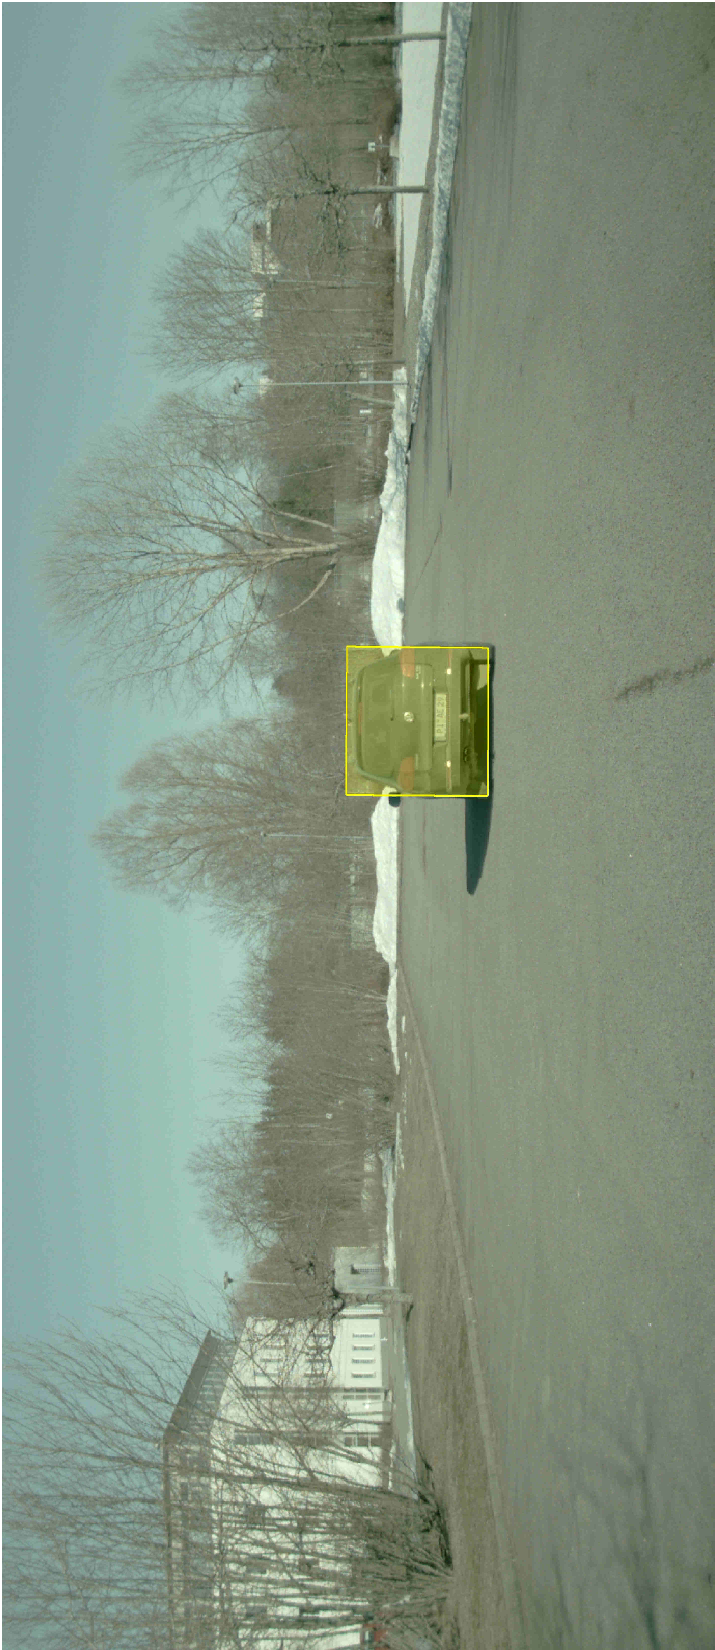
\includegraphics[angle=-90,origin=c,trim={0 0 15cm 0},width=0.9\textwidth]{roi_example}};
		\draw[red, very thick, <->] (0.2,0.2) -- (1.25,0.2) node[pos = 0.5, anchor=south] {$p_\text{Width}$};
	\end{tikzpicture}
	\caption{\label{fig:roiwidth} The \abbrROI width measurement from real-world data.}
\end{figure}

\newpage

\subsection{ROI Bottom Measurement}

The bottom of the \abbrROI can also be used as a measurement.
The measurement equation, according to \Figureref{fig:measurementmodelbottom}, then becomes
%
\begin{equation}
\begin{split}
    p_{\text{Bottom, back}} &= -f_v \frac{z + (0,0,1) \rotmat(\psi) (- \alpha l,0,0)^T}{x + (1,0,0) \rotmat(\psi) (- \alpha l,0,0)^T} + e_{\text{Bottom, back}} \\
    &= -f_v \frac{z}{x - \alpha l \cos(\psi)} + e_{\text{Bottom, back}},
\end{split}
\end{equation}
%
where $e_{\text{Bottom, back}}$ is the measurement noise.
The measurement is the number of pixels offset for the bottom position, compared to the center of the image in the $v$-direction.
This is illustrated in \Figureref{fig:roibottom}.
If instead the front of the target is observed, the factor $\alpha$ is changed to $\alpha-1$ and the measurement equation becomes
%
\begin{equation}
    p_{\text{Bottom, front}} =  -f_v \frac{z}{x - (\alpha - 1) l \cos(\psi)} + e_{\text{Bottom, front}},
\end{equation}
where $e_{\text{Bottom, front}}$ is the measurement noise.

% ROI Bottom
\begin{figure}[!ht]
    \centering
    \begin{tikzpicture}[scale=0.8, every node/.style={scale=0.8}]
        % --- Draw image plane ---
        \draw[very thick] (0,3) node[anchor=south] {Image plane} -- (0,-2);
        % ---

        % --- Draw host vehicle and associated lines---
        \draw (-6,-1) rectangle (-3,1) node[pos=0.5] {Host};
        \draw (-3,0.8) -- (3,0.8) -- (3,-1) -- cycle;
        \draw (-0.25,-0.1) -- (0.6,-0.1);
        \draw[->] (0.5,0.8) -- (0.5,-0.1) node[pos=0.5, anchor=west] {$p_{bottom}$};
        \draw[->] (-3,1.2) -- (0,1.2) node[pos=0.5, anchor=south] {$f_v$};
        \draw[->] (-3,-1.2) -- (3,-1.2) node[pos=0.7, anchor=north] {$x - \alpha l \cos(\psi)$};
        % ---

        % --- Draw target vehicle and associated lines ---
        \draw (3,-1) rectangle (6,1) node[pos=0.5] {Target};
        \draw[->] (3.2,0.8) -- (3.2,-1) node[pos=0.5,anchor=west] {$-z$};
        % ---
    \end{tikzpicture}
    \caption{\label{fig:measurementmodelbottom} The measurement model for the \abbrROI bottom point when observing the back of the target.}
\end{figure}

\begin{figure}[!ht]
	\centering
	\begin{tikzpicture}
		\node[] at (0,0) {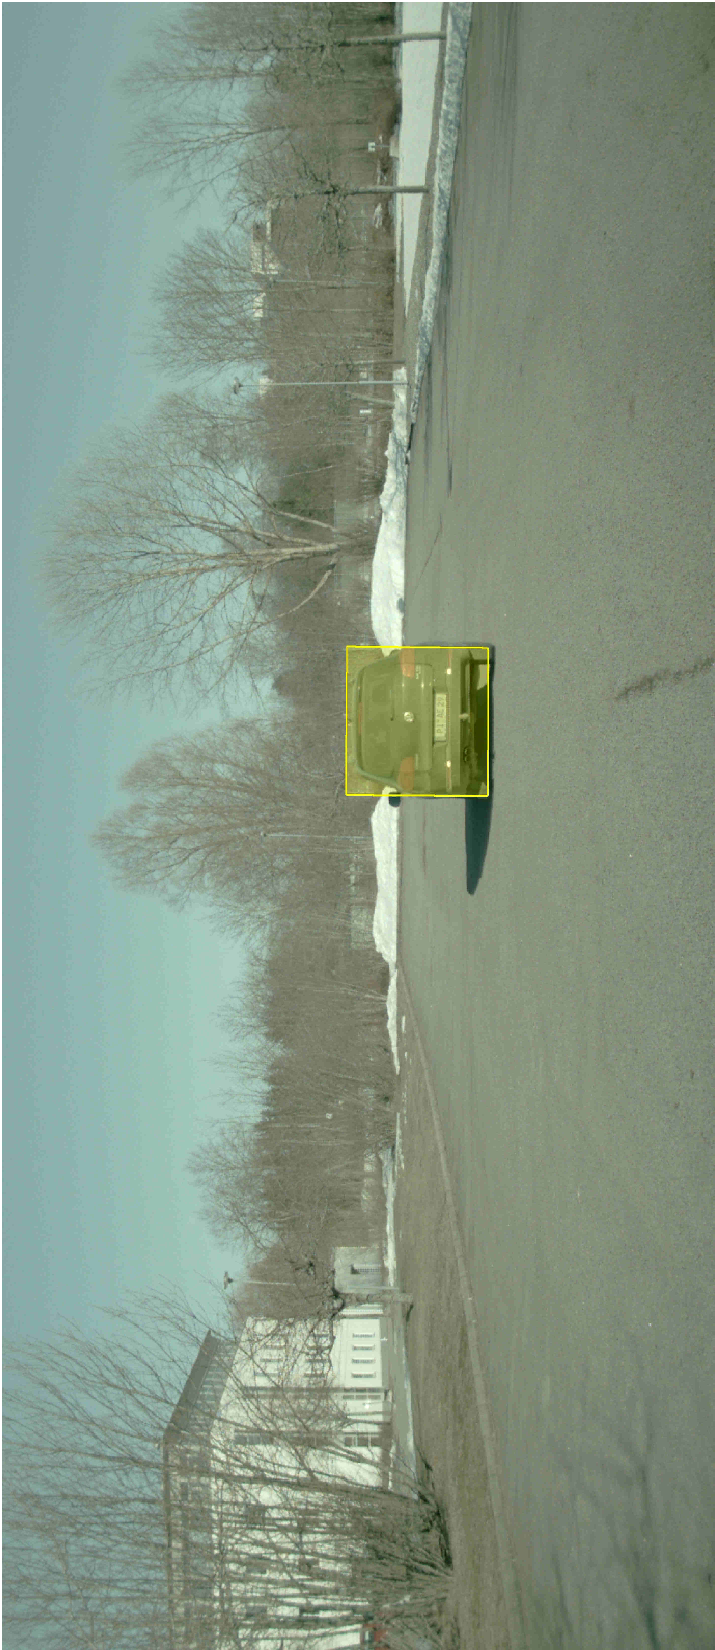
\includegraphics[angle=-90,origin=c,trim={0 0 15cm 0},width=0.85\textwidth]{roi_example}};
		\draw[red, very thick, |->] (0.65,0) -- (0.65,-0.75) node[pos = 0.5, anchor=west] {$p_\text{Bottom}$};
	\end{tikzpicture}
	\caption{\label{fig:roibottom} The \abbrROI bottom measurement from real-world data.}
\end{figure}

\newpage

\subsection{Angular Rate Measurements}
\label{sec:angratemeas}
By selecting feature points inside the lower half of the \abbrROI, and by using the knowledge about how pairs of feature points have moved between two images, the homography can be estimated.
The lower half of the \abbrROI was selected in order to get feature points lying on a planar surface.
The homography can be decomposed into a rotation matrix $\rotmat$, translation vector $\bm{t}$ and a plane normal vector $\bm{n}$.
Here, the plane normal is the normal of the plane before the homography transformation.
A brief overview of the decomposition will be presented here.
More details can be found in \cite{Malis:2007}.

The homography matrix $\bm{H}$ can be decomposed as
%
\begin{equation}
    \bm{H} = \rotmat + \bm{t} \bm{n}^T.
\end{equation}
%
The rotation matrix $\rotmat$ describes how the plane has rotated between two images.
Since the rotation is relative to the previous image, no absolute angle can be measured.
Instead, the rotation can be used to create the angular rate since the time between two images is assumed to be known, \ie the camera's frame rate.
By extracting the Euler angles from the rotation matrix, the angular rate can be calculated and used as a measurement.
The measurement equation simply becomes
%
\begin{equation}
	y_{\bm{H}} = \omega + e_{\bm{H}},
\end{equation}
%
where $e_{\bm{H}}$ is the measurement noise when using the homography $\bm{H}$ to construct the angular rate measurements.

As mentioned in both \cite{Gabb:2013} and \cite{Malis:2007}, there exist several solutions (up to eight) to the decomposition of the homography matrix.
One problem this method is facing is to decide which solution to choose.
In \cite{Malis:2007}, some methods are described to reduce the number of reasonable solutions from eight to two.
But still, there exists no method to decide the final solution.

Here, some alternatives are proposed on how to select the final solution.
%
\begin{itemize}
    \item Select the solution closest to the current state of the angular rate.

    This will tend to conserve the current state and could fail to detect a sudden change in the angular rate.

    \item Select the solution which has the smallest absolute angular rate.

    Since cars do not usually turns very sharply, one can argue for always choosing the smallest absolute angular rate to be a reasonable alternative.

    \item Use both solutions in the filter and later decide which track to drop.

    Use both measurements and run two parallel hypotheses until one is more likely then the other, and than discard the least likely one.
    This method will however generate an exponential growth of hypotheses.
    This must be taken into consideration if this particular alternative is selected.

    \item Perform empirical studies on synthetic data and see if there is a pattern.

    By using simulated data, the ground truth and the correct decomposition is known and the selected solution can be verified.
\end{itemize}

\subsection{Corner Measurements}
In order to get better information about the heading of the target, using measurements from the corners of the target should improve the estimation.
The available corners for measurements can be seen in \Figureref{fig:measurementmodelcorners} and a hypothetical example from real-world data can be seen in \Figureref{fig:corners}.
The measurement equations can be constructed by writing the \spacedim{3} coordinates of each of the four corners and then project them onto the image plane.
They can be projected in both the image $u$-direction and $v$-direction.

These types of measurements in world coordinates can easily be obtained with a stereo camera system, since it has access to depth information from the disparity image.
The purpose of introducing these measurements into the mono camera system, is to show what performance could be expected if these types of measurements would be available there as well.
Although, the measurements would be in image coordinates rather than in world coordinates.

The equations of the \spacedim{3} positions of the corners are
%
\begin{align}
	\text{RR}^{\text{\spacedim{3}}} &=
	\left( x,  y, z \right)^T + \rotmat(\psi) \, \left( -\alpha l, \, -w/2, \, 0 \right)^T, \\
	\text{RL}^{\text{\spacedim{3}}} &=
	\left( x,  y, z \right)^T + \rotmat(\psi) \, \left( -\alpha l, \, w/2, \, 0 \right)^T, \\
	\text{FR}^{\text{\spacedim{3}}} &=
	\left( x,  y, z \right)^T + \rotmat(\psi) \; \big( (1-\alpha)l, \, -w/2, \, 0 \big)^T, \\
	\text{FL}^{\text{\spacedim{3}}} &=
	\left( x,  y, z \right)^T + \rotmat(\psi) \; \big( (1-\alpha)l, \, w/2, \, 0 \big)^T.
\end{align}
%
By using the pinhole camera model and projecting the \spacedim{3} positions onto the image plane, the resulting measurement equations for the image $u$-coordinate of the corners are
%
\begin{align}
	p^\text{RR}_u &= -f_u \frac{\text{RR}_y^{\text{\spacedim{3}}}}{\text{RR}_x^{\text{\spacedim{3}}}} + e^\text{RR}_u, \\
	p^\text{RL}_u &= -f_u \frac{\text{RL}_y^{\text{\spacedim{3}}}}{\text{RL}_x^{\text{\spacedim{3}}}} + e^\text{RL}_u, \\
	p^\text{FR}_u &= -f_u \frac{\text{FR}_y^{\text{\spacedim{3}}}}{\text{FR}_x^{\text{\spacedim{3}}}} + e^\text{FR}_u, \\
	p^\text{FL}_u &= -f_u \frac{\text{FL}_y^{\text{\spacedim{3}}}}{\text{FL}_x^{\text{\spacedim{3}}}} + e^\text{FL}_u,
\end{align}
%
where $e^\text{RR}_u, e^\text{RL}_u, e^\text{FR}_u$ and $e^\text{FL}_u$ is the measurement noise, respectively.
The same strategy could also be used to get the $v$-coordinates in the image by interchanging $f_u$ to $f_v$ and $\text{RR}_y^\text{\spacedim{3}}$ to $\text{RR}_z^\text{\spacedim{3}}$ etc.

\begin{figure}[!ht]
    \centering
    \begin{tikzpicture}[scale=1.2, every node/.style={scale=1.2}]
        % --- Draw rectangle car ---
        \draw (0,0) node[anchor=north west] {RL} node[circle,fill,inner sep=1.5pt] {}  -- (3,1) node[anchor=north west] {RR} node[circle,fill,inner sep=1.5pt] {} -- (1.5,5.5) node[anchor=west] {FR} node[circle,fill,inner sep=1.5pt] {} -- (-1.5,4.5) node[anchor=east] {FL} node[circle,fill,inner sep=1.5pt] {} -- cycle;
        \draw[dashed] (-0.5,1.5) -- (2.5,2.5) node[pos=0.6, anchor=north] {$(x,y,z)$};
        \draw[->] (1,2) node[circle,fill,inner sep=1pt] {} -- (0.3,4) node[anchor=south] {$v$};
        \draw[dotted] (1,2) -- (1,4);
        \draw[<-] (0.65,3) .. controls (0.8,3.1) .. (1,3.1) node[pos=0.5, anchor=south] {$\psi$};
        % ---

        % --- Draw lines for length and width ---
        \draw[<->] (-0.25,-0.1) -- (-0.75,1.4) node[pos=0.5, anchor=east] {$\alpha l$};
        \draw[<->] (-0.75,-0.3) -- (-2.25,4.2) node[pos=0.5, anchor=east] {$l$};
        \draw[<->] (-1.6,4.8) -- (1.4,5.8) node[pos=0.5, anchor=south] {$w$};
        % ---
    \end{tikzpicture}
    \caption{\label{fig:measurementmodelcorners} Measurement model of the corners available to measure on the target.}
\end{figure}

\hfill

\begin{figure}[!ht]
	\centering
	\begin{tikzpicture}
		\node[] at (0,0) {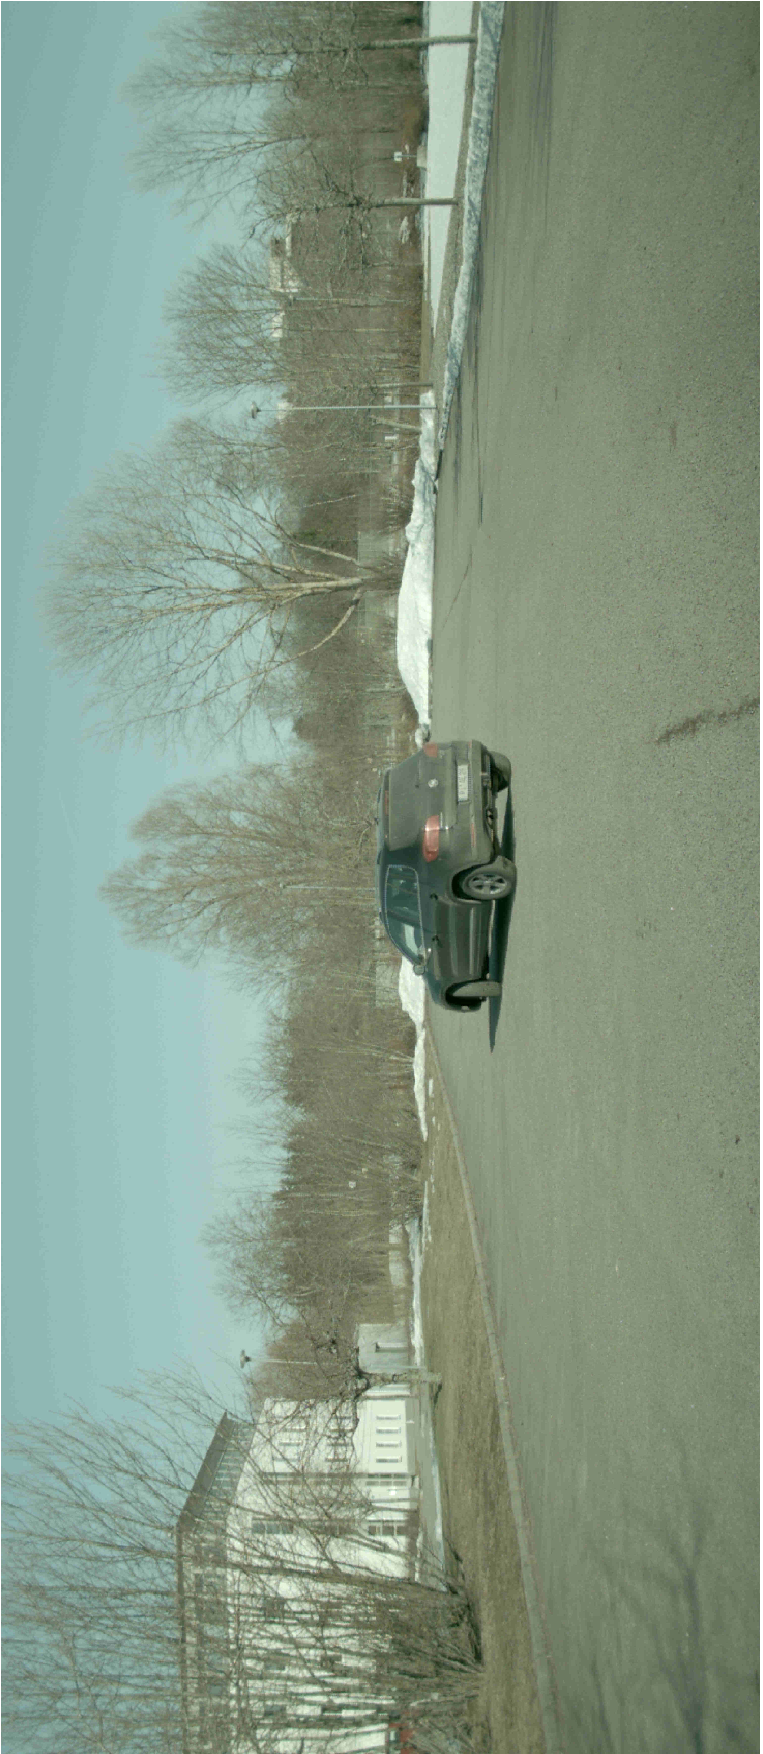
\includegraphics[angle=-90,origin=c,trim={0 0 16cm 0},width=0.9\textwidth]{corners_example}};
		\node[red,circle,fill,inner sep=1.5pt,label=left:{\color{red}FL}] at (-0.85,-0.65) {};
		\node[red,circle,fill,inner sep=1.5pt,label=below:{\color{red}RL}] at (0.2,-0.85) {};
		\node[red,circle,fill,inner sep=1.5pt,label=right:{\color{red}RR}] at (0.85,-0.75) {};
	\end{tikzpicture}
	\caption{\label{fig:corners} An example of what the measurements from corners could look like.}
\end{figure}

\clearpage

\section{Rotation Estimation with EKF}
Using the motion model and measurement models defined in the preceding sections, the heading can be estimated using the \abbrEKF and by applying \Algorithmref{algo:ekf}.
The state vector is
\begin{equation*}
	\bm{x} =
	\begin{pmatrix}
		x & y & z & v & \psi & \omega
	\end{pmatrix}
	^T
	,
\end{equation*}
and the measurement vector is
\begin{equation*}
	\bm{y} =
	\begin{pmatrix}
		\text{\abbrROI horizontal center position} \\
		\text{\abbrROI bottom} \\
		\text{\abbrROI width} \\
		\text{Angular rate} \\
		\text{Corner coordinates in } u \\
		\text{Corner coordinates in } v
	\end{pmatrix}
	.
\end{equation*}
The process and measurement noise covariance matrices $\bm{Q}$ and $\bm{R}$ are tuning parameters which have to be manually tuned in order to get a good state estimate.

\section{Observability of the Filter}
\label{sec:observabilitymethod}
In order to know if it is possible to get a reasonable solution with the proposed filter structure, the theory from \Sectionref{sec:obsanalysis} is applied.
Since the filter is nonlinear, one can only achieve an observability result around a certain trajectory.
This means that it is not possible to make a general conclusion about the observability of the filter.
Although, by simulating a number of trajectories which could represent interesting real-world scenarios, at least something can be said about the observability.

The Jacobians in each frame in the trajectory have to be calculated and then \eqref{eq:observabilitytheorem} in \Theoremref{th:observability} can be applied to calculate the observability Gramian of the trajectory.
In order to check if the observability Gramian is invertible, the rank of the matrix can be investigated in each sample.

\section{Monte Carlo Simulations}
One way to get knowledge about the expected performance of the filter, is to use the Monte Carlo method, \ie run simulations multiple times and calculate the mean of all observed results (\abbrRMSE).
By first simulating a trajectory and generating measurements accordingly, one can use the generated measurements to estimate the simulated trajectory.
This enables several things:
\begin{itemize}
	\item The simulated trajectory works as ground truth.
	\item All kinds of trajectories can be simulated.
	\item The noise levels of the measurements are controllable.
	\item The expected performance of the filter can be measured.
\end{itemize}
Using the Monte Carlo method, the same trajectory is simulated multiple times with different noise realizations and the mean of the \abbrRMSE's of the estimated trajectories are calculated.
In this thesis, the number of Monte Carlo runs for each trajectory were selected to 1000.

\chapter{Performance Evaluation}
\label{cha:result}
The filter has been evaluated in several different ways.
To get an idea of if the filter has a reasonable formulation or not, an initial observability analysis has been done.
Because if the filter formulation is not plausible, a reformulation of the problem might be necessary.
Monte Carlo simulations were then used to obtain some statistical properties, and a theoretical performance analysis, without having to calculate it analytically.
Since the filter depends on the quality of the constructed angular rate measurements, the selected homography estimation method has been evaluated through simulations.

To see how the filter perform compared to a stereo camera system, two sequence were recorded and the output has been compared with the output from the filter constructed in this thesis.

\section{Observability Along Different Trajectories}
\label{sec:observabilityresult}
In order to see if the filter is reasonably formulated, an observability analysis according to \Sectionref{sec:observabilitymethod} has been performed and summarized in \Tableref{tab:observabilityresult}.
The results show that the filter is formulated such that a trajectory with a moving target seems to be observable.
A trajectory of a target with no ego motion is observable only if all three kind of measurements are available.
It is not observable if only \abbrROI and angular rate measurements are available.

\begin{table}[!ht]
	\centering
	\caption{\label{tab:observabilityresult} A summary of the observability analysis results for different trajectories and different measurement setups.}
	\begin{tabular}{|p{5cm}|p{1cm}|p{2cm}|p{2.5cm}|}
		\cline{2-4}
		\multicolumn{1}{c|}{} & \multicolumn{3}{c|}{\textbf{Observable}} \\
		\hline
		\textbf{Description} & \abbrROI & \abbrROI and angular rate & \abbrROI, angular rate and corners \\
		\hline
		The target is standing still with an arbitrary initial yaw angle. & No & No & Yes \\
		\hline
		The target is driving straight towards or straight away from the host. & Yes & Yes & Yes \\
		\hline
		The target is driving towards or away from the host applying sine steering. & Yes & Yes & Yes \\
		\hline
		The target is driving away from the host and makes a $45^\circ$ turn. & Yes & Yes & Yes \\
		\hline
		The target is driving across the host's lane with constant speed and constant yaw angle. & Yes & Yes & Yes \\
		\hline
	\end{tabular}
\end{table}

A intuitive explanation to why that particular situation is not observable is that, if the target has no ego motion and only \abbrROI and angular rate are used as measurements, the same \abbrROI measurements could be observed from several different target state vectors.
For example could the same \abbrROI appear if the target is rotated either $\pm\psi$ and the $(x,y,z)^T$ position is adjusted accordingly.
The \abbrROI will appear the same in the image plane.

Since it is difficult to prove general observability for nonlinear systems, these results at least gives a hint that the problem is reasonably formulated.
The filter should, in the selected test cases where the target had an ego motion, be able to estimate the given trajectory.

\newpage

\section{Monte Carlo Simulations}
\label{sec:montecarloresult}
By first simulating the filter using the Monte Carlo method, a rough evaluation of the filter's performance can be obtained.
By using Monte Carlo simulations, the available measurements and the measurement noise levels can be controlled.
It is always good to know what to strive for when running the filter on real-world data.
The goal of performing the Monte Carlo simulations is to get results about what qualities on the measurements that are required in order to get a good state estimate, especially regarding the angular rate measurements.

Two different scenarios were simulated, with different noise realisations.
The applied noise was Gaussian, with zero mean and different covariance matrices.
The covariance matrices $\bm{Q}^\text{sim}$ and $\bm{R}^\text{sim}$ were used when simulating the trajectory and generating the measurements while $\bm{Q}$ and $\bm{R}$ were used when estimating the trajectory.
The simulation covariance matrices were
\begin{align}
	\label{eq:Qsim}
	\bm{Q}^\text{sim} &=
	\begin{pmatrix}
		0 & 0 & 0 & 0 & 0 & 0 \\
		0 & 0 & 0 & 0 & 0 & 0 \\
		0 & 0 & 0 & 0 & 0 & 0 \\
		0 & 0 & 0 & 0.0001 & 0 & 0 \\
		0 & 0 & 0 & 0 & 0 & 0 \\
		0 & 0 & 0 & 0 & 0 & Q^\text{sim}_\omega
	\end{pmatrix}
	,
	\\
	\label{eq:Rsim}
	\bm{R}^\text{sim} &=
	\begin{pmatrix}
		10 & 0 & 0 & 0 & 0 & 0 \\
		0 & 10 & 0 & 0 & 0 & 0 \\
		0 & 0 & 10 & 0 & 0 & 0 \\
		0 & 0 & 0 & R^\text{sim}_\omega & 0 & 0 \\
		0 & 0 & 0 & 0 & 10 & 0 \\
		0 & 0 & 0 & 0 & 0 & 10
	\end{pmatrix}
	.
\end{align}
The $\bm{Q}$ and $\bm{R}$ matrices were tuned in order to get good state estimates.
The initial state, $\bm{x}_0$, of the target was set to
%
\begin{equation*}
	\bm{x}_0 =
	\begin{pmatrix}
		p_\text{Bottom} & p_\text{HCP} & -1.5 & 0 & 0 & 0
	\end{pmatrix}^T.
\end{equation*}
%
Here, $p_\text{Bottom}$ and $p_\text{HCP}$ means that the measurement equations for the \abbrROI bottom and \abbrROI horizontal center position were used to initialize the $x$ and $y$ states, respectively.

\newpage

First, a simulation of a target detected 15 meters in front of the host, driving straight away with a constant velocity of 5 m/s, was evaluated.
The used measurements and the parameters $Q^\text{sim}_\omega$ and $R^\text{sim}_\omega$ varied according to \Tableref{tab:montesimscenario1}.
%
\begin{table}[!ht]
	\centering
	\caption{\label{tab:montesimscenario1} The simulation parameters and available measurements for different setup cases of the first simulated scenario.}
	\renewcommand{\arraystretch}{1.2}
	\begin{tabular}{|l|p{3.5cm}|l|l|}
		\hline
		\textbf{Setup no.} & \textbf{Measurements} & $Q^\text{sim}_\omega$ (rad/s) & $R^\text{sim}_\omega$ (rad/s) \\
		\hline
		1 & \abbrROI & $1.7\cdot 10^{-6}$ & -- \\
		\hline
		2 & \abbrROI and angular rate & $1.7\cdot 10^{-6}$ & 0.1 \\
		\hline
		3 & \abbrROI and angular rate & $1.7\cdot 10^{-6}$ & 0.5 \\
		\hline
		4 & \abbrROI and angular rate & $1.7\cdot 10^{-6}$ & 1 \\
		\hline
		5 & \abbrROI, angular rate and corners & $1.7\cdot 10^{-6}$ & 0.1 \\
		\hline
	\end{tabular}
\end{table}

In this scenario, the covariance matrices $\bm{Q}$ and $\bm{R}$ were
\begin{align}
	\label{eq:Qsim1}
	\bm{Q} &=
	\begin{pmatrix}
		0.25 & 0 & 0 & 0 & 0 & 0 \\
		0 & 0.1 & 0 & 0 & 0 & 0 \\
		0 & 0 & 0.05 & 0 & 0 & 0 \\
		0 & 0 & 0 & 1 & 0 & 0 \\
		0 & 0 & 0 & 0 & 0.00017 & 0 \\
		0 & 0 & 0 & 0 & 0 & 0.0017 \\
	\end{pmatrix}, \\
	\label{eq:Rsim1}
	\bm{R} &= 10 \bm{R}^\text{sim},
\end{align}
in all setup cases.
The matrix $\bm{R}^\text{sim}$ is given by \eqref{eq:Rsim}.

The results for each setup can be seen in \Figureref{fig:27montesimstraighttowardsroirmse}, \Figureref{fig:20montesimstraighttowardsroiangvelrmse}, \Figureref{fig:21montesimstraighttowardsroiangvelrmse}, \Figureref{fig:22montesimstraighttowardsroiangvelrmse} and \Figureref{fig:30montesimstraighttowardsroiangvelcornerrmse}.
Examples of the simulated trajectories can be found in \Figureref{fig:27montesimstraighttowardsroitrajpos}, \Figureref{fig:27montesimstraighttowardsroitrajother}, \Figureref{fig:20montesimstraighttowardsroiangveltrajpos}, \Figureref{fig:20montesimstraighttowardsroiangveltrajother}, \Figureref{fig:30montesimstraighttowardsroiangvelcornertrajpos} and \Figureref{fig:30montesimstraighttowardsroiangvelcornertrajother} in \Appendixref{app:montecarlo}.

If only \abbrROI measurements were used, the filter performed poorly as can be seen in \Figureref{fig:27montesimstraighttowardsroirmse}.
Especially regarding the orientation, \ie the yaw angle.
If additionally to the \abbrROI measurement, angular rate measurements were added, a significant improvement were obtained, as can be seen in \Figureref{fig:20montesimstraighttowardsroiangvelrmse}.
Here, the noise variance level were 0.1 rad/s.
In \Figureref{fig:21montesimstraighttowardsroiangvelrmse} and \Figureref{fig:22montesimstraighttowardsroiangvelrmse}, the \abbrRMSE of the estimated states diverged quickly due to the high noise level of the angular rate measurements.
The noise variance levels were 0.5 rad/s and 1 rad/s, respectively.
Note especially the difference in the yaw angle comparing \Figureref{fig:20montesimstraighttowardsroiangvelrmse} with \Figureref{fig:21montesimstraighttowardsroiangvelrmse} and \Figureref{fig:22montesimstraighttowardsroiangvelrmse}.
The idea of adding the measurements of the target's corners, considering \Figureref{fig:30montesimstraighttowardsroiangvelcornerrmse}, resulted in an excellent state estimate.

\begin{figure}[!ht]
	\centering
	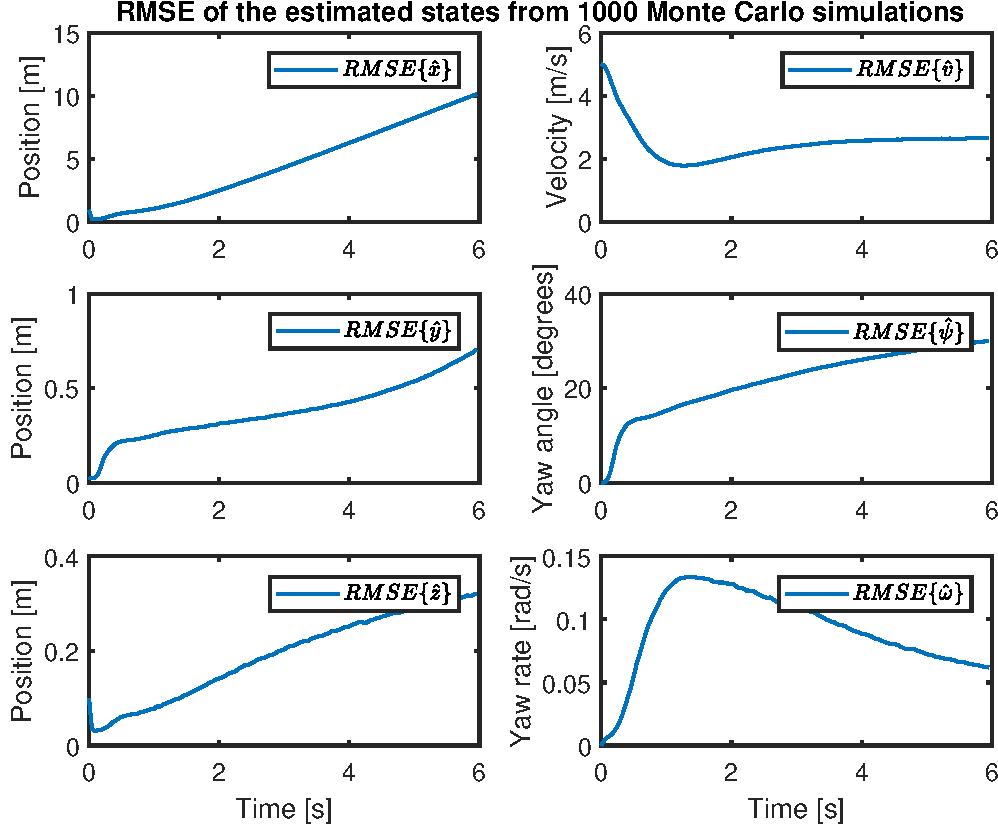
\includegraphics[width=0.8\textwidth]{MonteCarloSim/27_MC_1000_Rmse}
	\caption{\label{fig:27montesimstraighttowardsroirmse} Monte Carlo simulation result of scenario 1 with setup 1.}
\end{figure}

\begin{figure}[!ht]
	\centering
	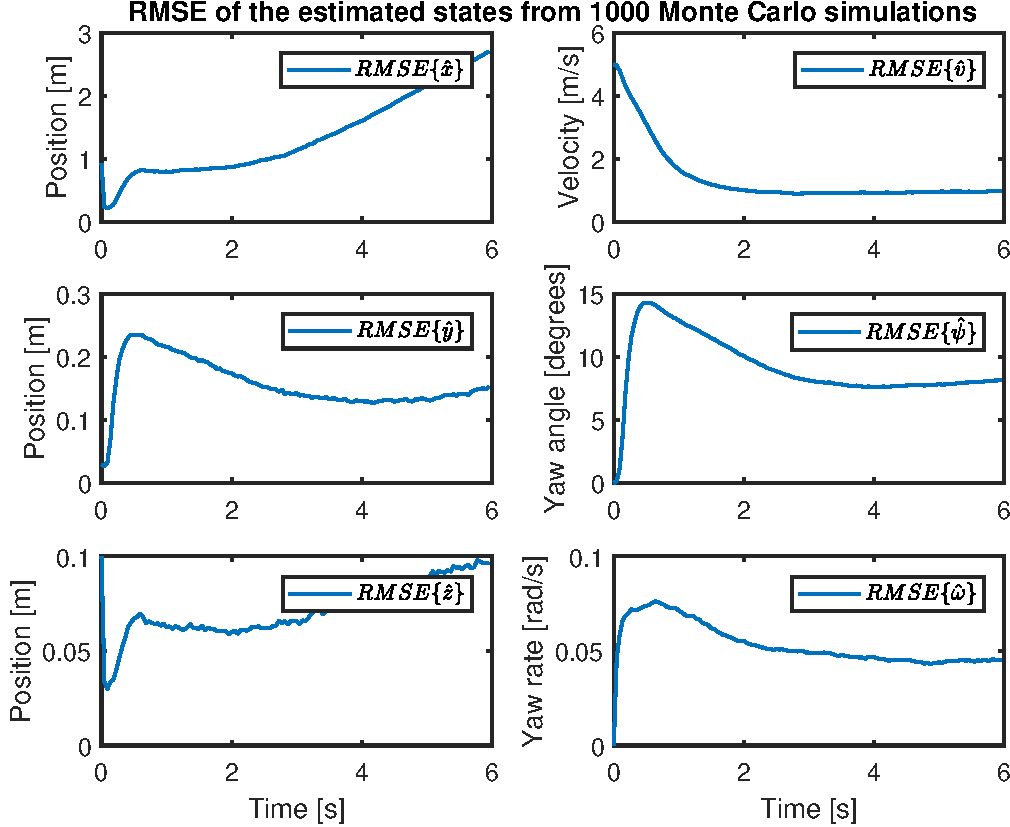
\includegraphics[width=0.8\textwidth]{MonteCarloSim/20_MC_1000_Rmse}
	\caption{\label{fig:20montesimstraighttowardsroiangvelrmse} Monte Carlo simulation result of scenario 1 with setup 2.}
\end{figure}

\begin{figure}[!ht]
	\centering
	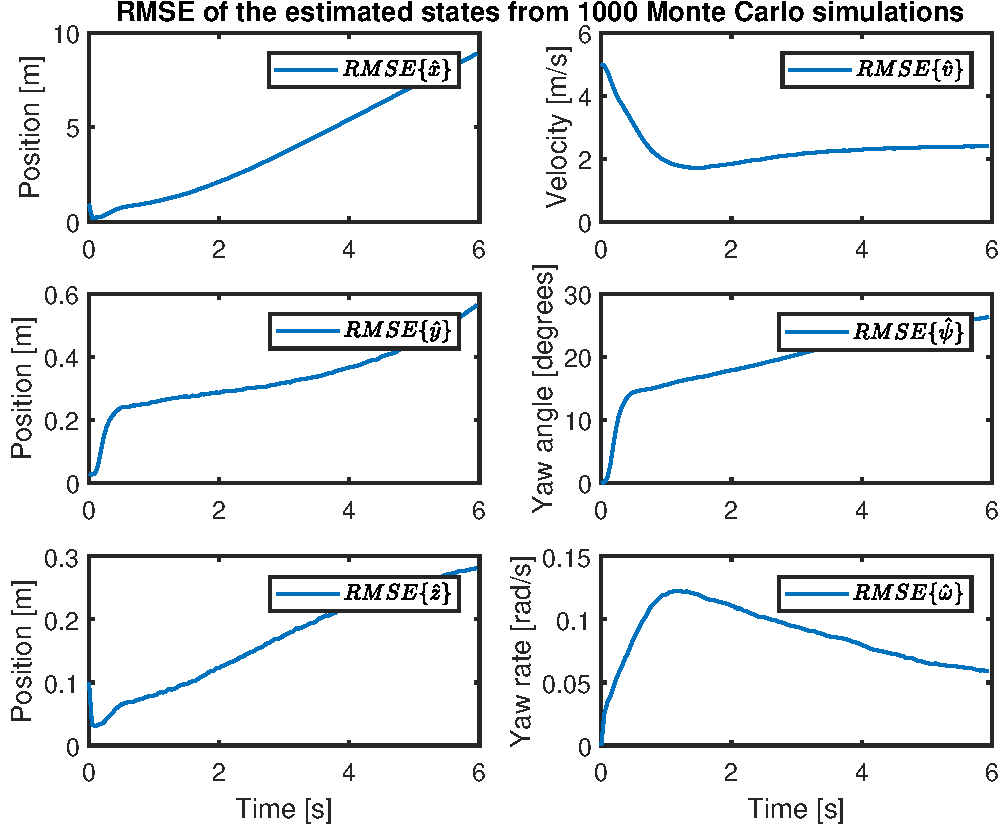
\includegraphics[width=0.8\textwidth]{MonteCarloSim/21_MC_1000_Rmse}
	\caption{\label{fig:21montesimstraighttowardsroiangvelrmse} Monte Carlo simulation result of scenario 1 with setup 3.}
\end{figure}

\begin{figure}[!ht]
	\centering
	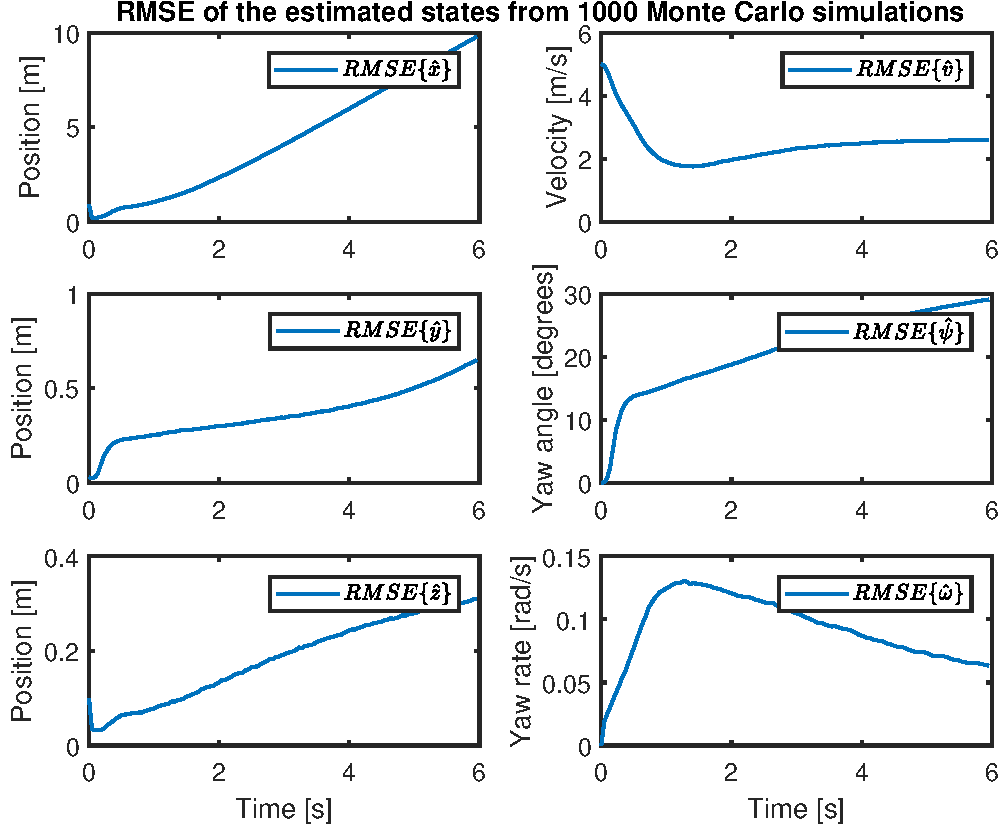
\includegraphics[width=0.8\textwidth]{MonteCarloSim/22_MC_1000_Rmse}
	\caption{\label{fig:22montesimstraighttowardsroiangvelrmse} Monte Carlo simulation result of scenario 1 with setup 4.}
\end{figure}

\begin{figure}[!ht]
	\centering
	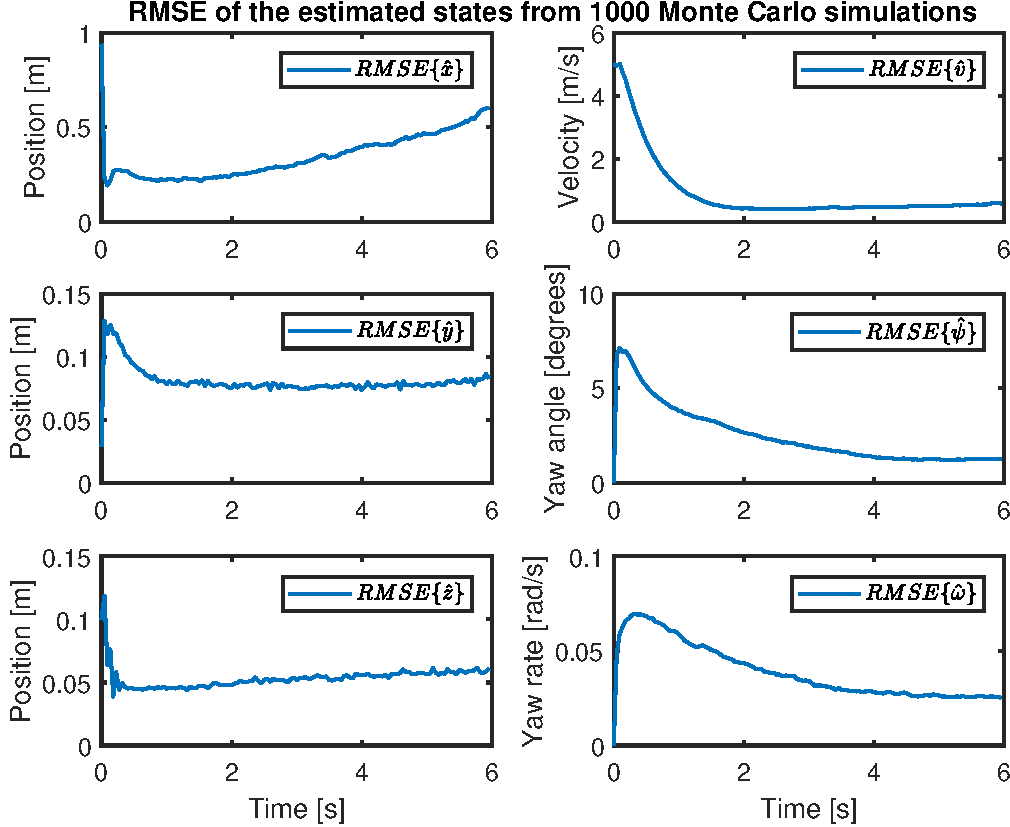
\includegraphics[width=0.8\textwidth]{MonteCarloSim/30_MC_1000_Rmse}
	\caption{\label{fig:30montesimstraighttowardsroiangvelcornerrmse} Monte Carlo simulation result of scenario 1 with setup 5.}
\end{figure}

\clearpage

Secondly, a simulation of a target (detected 15 meters in front of the host) performing a turn to the right, was evaluated.
The target drove with a constant velocity of 4 m/s and after 2 seconds, it performed a turn to the right.
The used measurements and the parameters $Q^\text{sim}_\omega$ and $R^\text{sim}_\omega$ varied according to \Tableref{tab:montesimscenario2}.

\begin{table}[!ht]
	\centering
	\caption{\label{tab:montesimscenario2} The simulation parameters and available measurements for different setup cases of the second simulated scenario.}
	\renewcommand{\arraystretch}{1.2}
	\begin{tabular}{|l|p{3.5cm}|l|l|}
		\hline
		\textbf{Setup no.} & \textbf{Measurements} & $Q^\text{sim}_\omega$ (rad/s) & $R^\text{sim}_\omega$ (rad/s) \\
		\hline
		6 & \abbrROI & $1.7\cdot 10^{-6}$ & -- \\
		\hline
		7 & \abbrROI and angular rate & $1.7\cdot 10^{-6}$ & 0.1 \\
		\hline
		8 & \abbrROI and angular rate & $1.7\cdot 10^{-6}$ & 0.5 \\
		\hline
		9 & \abbrROI and angular rate & $1.7\cdot 10^{-6}$ & 1 \\
		\hline
		10 & \abbrROI, angular rate and corners & $1.7\cdot 10^{-6}$ & 0.1 \\
		\hline
	\end{tabular}
\end{table}

In this scenario, the covariance matrices $\bm{Q}$ and $\bm{R}$ were
\begin{align}
	\label{eq:Qsim2}
	\bm{Q} &=
	\begin{pmatrix}
		0.25 & 0 & 0 & 0 & 0 & 0 \\
		0 & 0.1 & 0 & 0 & 0 & 0 \\
		0 & 0 & 0.05 & 0 & 0 & 0 \\
		0 & 0 & 0 & 1 & 0 & 0 \\
		0 & 0 & 0 & 0 & 0.00017 & 0 \\
		0 & 0 & 0 & 0 & 0 & 0.0017 \\
	\end{pmatrix}, \\
	\label{eq:Rsim2}
	\bm{R} &= 10 \bm{R}^\text{sim},
\end{align}
in all setup cases.
The matrix $\bm{R}^\text{sim}$ is given by \eqref{eq:Rsim}.

The results for each setup can be seen in \Figureref{fig:13montesimcrossingroirmse}, \Figureref{fig:23montesimcrossingroiangvelrmse}, \Figureref{fig:24montesimcrossingroiangvelrmse}, \Figureref{fig:25montesimcrossingroiangvelrmse} and \Figureref{fig:29montesimcrossingroiangvelcornerrmse}.
Examples of the simulated trajectories can be found in \Figureref{fig:13trajectorycrossingroipos}, \Figureref{fig:13trajectorycrossingroiother}, \Figureref{fig:23trajectorycrossingroiangvelpos}, \Figureref{fig:23trajectorycrossingroiangvelother}, \Figureref{fig:29trajectorycrossingroiangvelcornerpos} and \Figureref{fig:29trajectorycrossingroiangvelcornerother} in \Appendixref{app:montecarlo}.

\Figureref{fig:13montesimcrossingroirmse} shows that if only \abbrROI measurements are used, a large \abbrRMSE were obtained of the estimated states.
The large \abbrRMSE of the angular rate state during the turn affects the rest of the states, especially the yaw angle.
In the simulation, as in the first scenario, the results gets improved by adding angular rate measurements.
In \Figureref{fig:23montesimcrossingroiangvelrmse}, the angular rate noise variance level were 0.1 rad/s.
If the angular rate measurements had too high noise variance level, the \abbrRMSE of the estimated state started to diverge, as in \Figureref{fig:24montesimcrossingroiangvelrmse} and \Figureref{fig:25montesimcrossingroiangvelrmse}.
The angular rate measurements variance noise levels were 0.5 rad/s and 1 rad/s, respectively.
As well as in the previous simulation, the result got significantly improved by adding the measurements of the target's corners, considering \Figureref{fig:29montesimcrossingroiangvelcornerrmse}.

\begin{figure}[!ht]
	\centering
	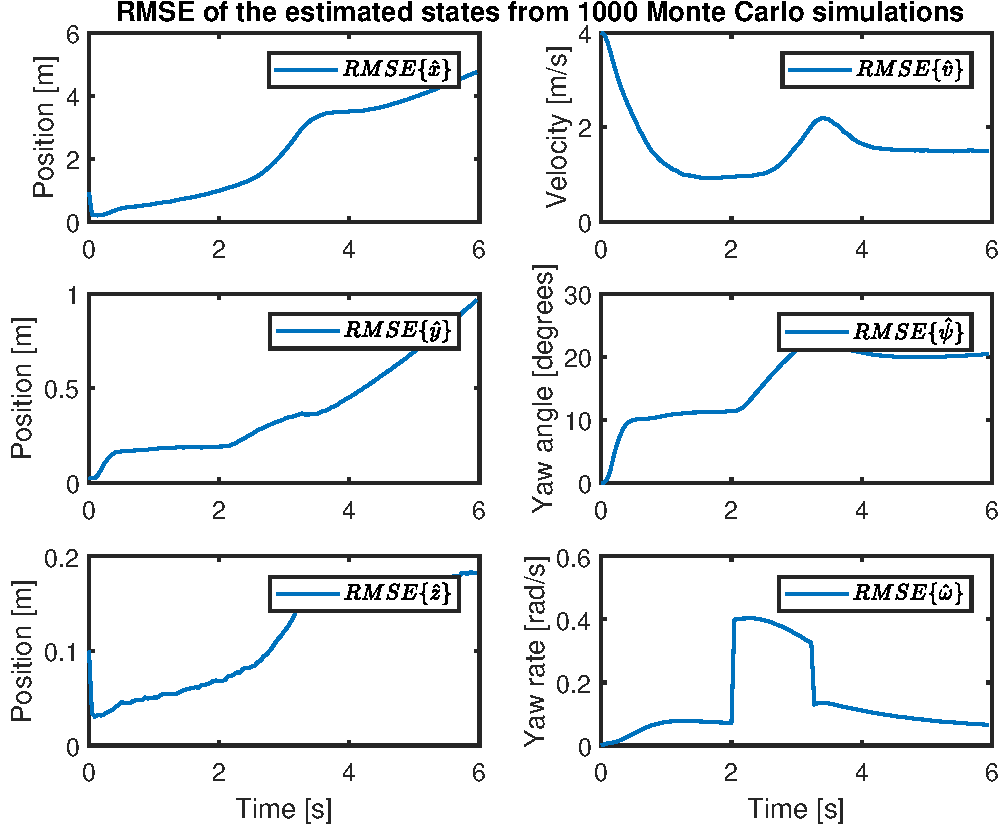
\includegraphics[width=0.8\textwidth]{MonteCarloSim/13_MC_1000_Rmse}
	\caption{\label{fig:13montesimcrossingroirmse} Monte Carlo simulation result of scenario 2 with setup 6.}
\end{figure}

\begin{figure}[!ht]
	\centering
	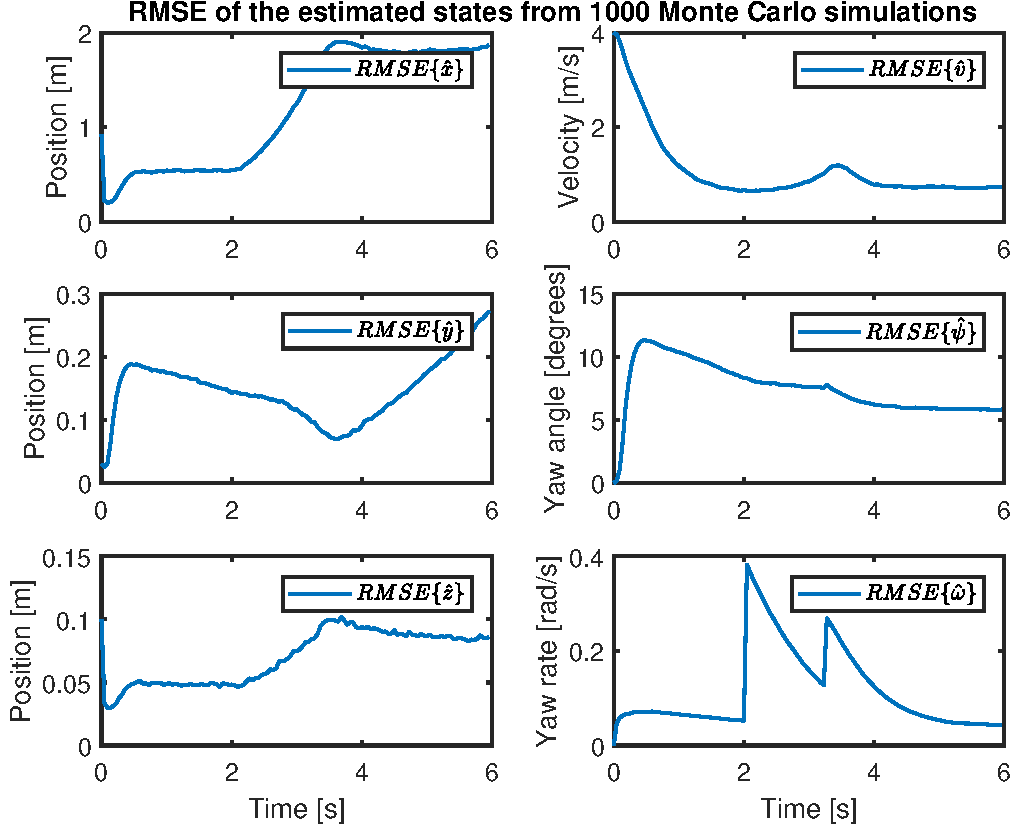
\includegraphics[width=0.8\textwidth]{MonteCarloSim/23_MC_1000_Rmse}
	\caption{\label{fig:23montesimcrossingroiangvelrmse} Monte Carlo simulation result of scenario 2 with setup 7.}
\end{figure}

\begin{figure}[!ht]
	\centering
	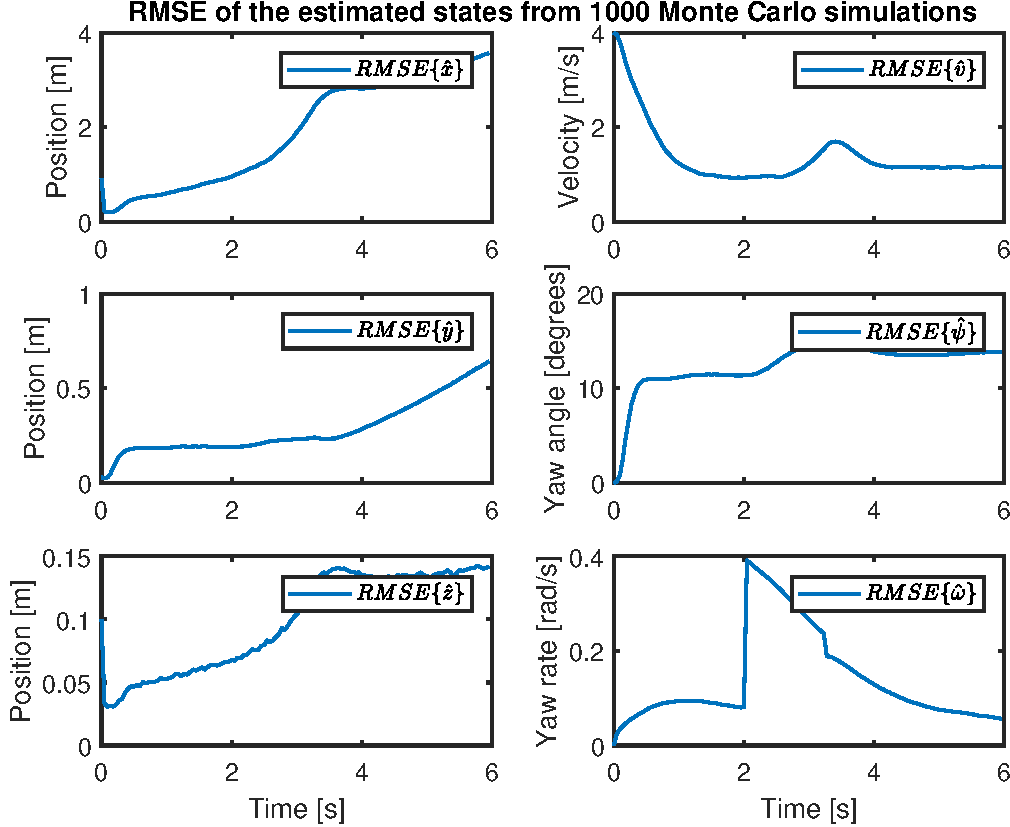
\includegraphics[width=0.8\textwidth]{MonteCarloSim/24_MC_1000_Rmse}
	\caption{\label{fig:24montesimcrossingroiangvelrmse} Monte Carlo simulation result of scenario 2 with setup 8.}
\end{figure}

\begin{figure}[!ht]
	\centering
	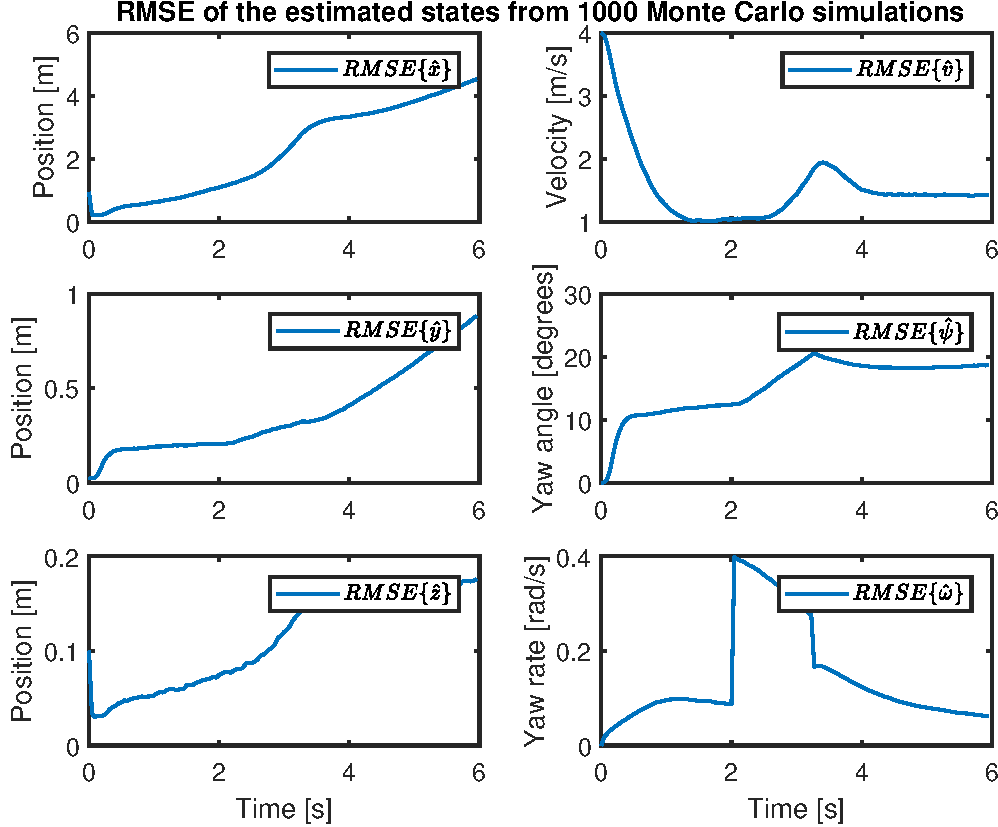
\includegraphics[width=0.8\textwidth]{MonteCarloSim/25_MC_1000_Rmse}
	\caption{\label{fig:25montesimcrossingroiangvelrmse} Monte Carlo simulation result of scenario 2 with setup 9.}
\end{figure}

\begin{figure}[!ht]
	\centering
	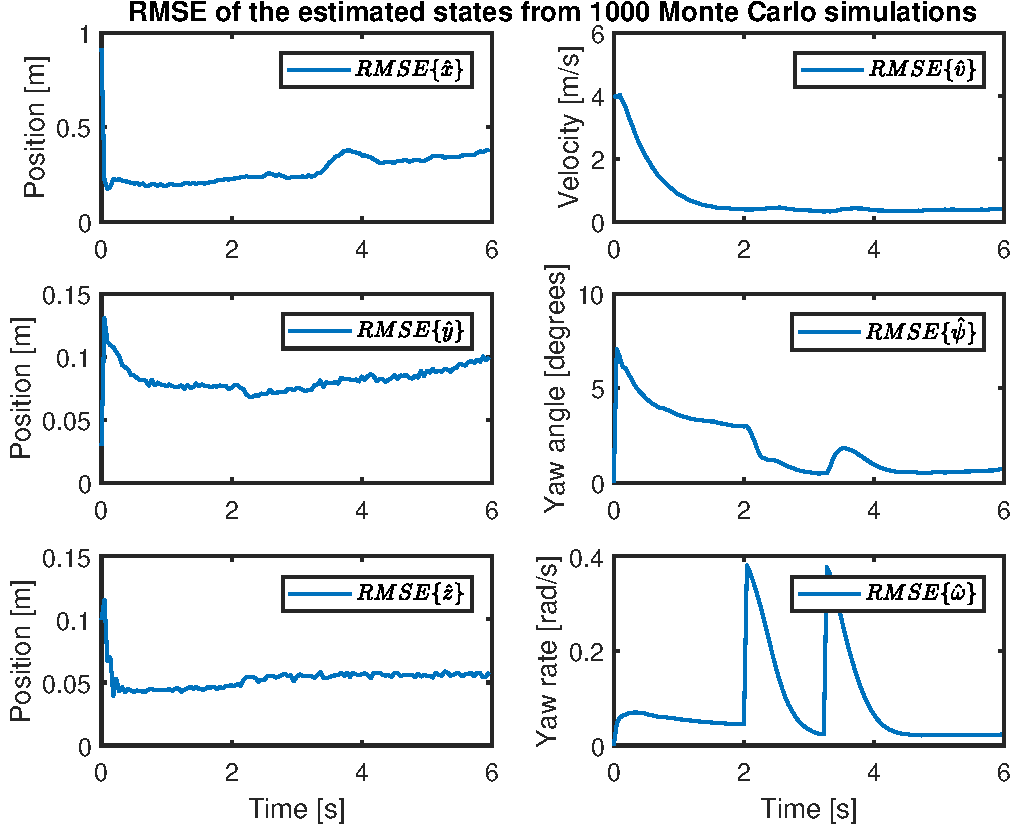
\includegraphics[width=0.8\textwidth]{MonteCarloSim/29_MC_1000_Rmse}
	\caption{\label{fig:29montesimcrossingroiangvelcornerrmse} Monte Carlo simulation result of scenario 2 with setup 10.}
\end{figure}

\newpage

The purpose of performing Monte Carlo simulations were to show which performance, \ie measurement noise level, that must be achieved in order to produce a good state estimated with the proposed filter structure.
This was especially interesting for the angular rate measurements.
From the two simulated scenarios, the results have shown that a measurement variance of 0.1 rad/s for the angular rate should be good enough.
A measurement noise variance of 0.5 rad/s is too large in order to obtain a good state estimate.

\newpage

\section{Homography Estimation}
\label{sec:homographyestimationresults}
It is of great interest to see how good homography estimations that can be achieved.
As can be seen from the Monte Carlo simulations in \Sectionref{sec:montecarloresult}, the angular rate measurements have the possibility to improve the result, if they have a low enough noise level.

Some experimenting on synthetic data has been performed in order to evaluate the result of the homography estimations.
A rectangle was created, and it used the same motion model as described in \eqref{eq:motionmodel}, to represent the possible backside of a target vehicle.
The tracked points on the rectangle were the four corner points and an additional number of randomly selected uniformly distributed points on the rectangle.
The rectangle performed a trajectory where it travelled straight away and then turned left.
In order to perturb the synthetic data, Gaussian noise was added when projecting the points on the rectangle onto the image plane.
This will make the points to not lie perfectly on the same plane.

To perform the homography estimations, \matlab mex functions that interfaced the OpenCV library \cite{mexopencv} were used, both when estimating the homography matrix $\bm{H}$ and when performing the decomposition into $\rotmat, \bm{t}$ and $\bm{n}$.

The results of the synthetic data simulation can be seen in \Figureref{fig:rectsim1e-2}, \Figureref{fig:rectsim5e-2}, \Figureref{fig:rectsim1e-1} and \Figureref{fig:rectsim5e-1}.
Different noise levels were used in each of the four simulations.
The number of tracked points inside the rectangle were 30 points in total for all the four simulations.
The rectangle was travelling with a constant velocity of 5 m/s and between frame number 35 and 65 it was performing a turn with a constant angular rate of 0.25 rad/s.
The distance travelled were between 5 to 30 meters.

By observing the result from the homography estimation with synthetic data, several things can be stated:
\begin{itemize}
	\item If the matching pixels do not match good enough, \ie the errors in matched pixel coordinates are too large, the quality of the estimated homography will be reduced.
	\item At a distance further away, the mismatching pixels will have an even larger effect on the homography estimation.
	\item If the target is far away, not even a small mismatch error might be good enough for estimating the homography, since the movement of the feature points is so small.
\end{itemize}

The same method were used when constructing the angular rate measurements from real-world data.
\Figureref{fig:angvelmeas} shows the angular rate measurements constructed from the estimated homographies with real-world data.
In \Figureref{fig:angvelmeas155532}, one can see that the angular rate measurements have a trend around 0 rad/s.
\Figureref{fig:angvelmeas155733} shows a negative trend of the angular rate measurements, since the target vehicle is turning to the right.
In order to have a comparison, the estimated angular rate state from a stereo camera system is shown in the same figure.

Looking at \Figureref{fig:angvelmeas}, some reasonable explanations to the noisy results could be that the feature point tracker does not perform good enough or that the selected feature point detector did not detect enough feature points.
Another explanation might be that the OpenCV implementation for finding and decomposing the homography matrix is too sensitive to noise, even though a \abbrRANSAC method (see \Sectionref{sec:ransac}) was utilized.

By further analysing the angular rate measurements from \Figureref{fig:angvelmeas}, their respectively variances could be calculated.
For the first sequence, a linear trend was subtracted from the measurements and the resulting variance was 0.8 rad/s.
For the seconds sequence, a nonlinear trend was subtracted from the measurements and the resulting variance was 2 rad/s.
This is too high variances compared to the required variance discussed in the previous section.
The evaluated sequences were recorded in clear daylight.
It reasonable to believe that the feature points will be even more difficult to track in bad light or in bad weather conditions.

The detection and tracking of feature points where implemented using \matlab's computer vision system toolbox.
For feature point detection, the minimum eigenvalue algorithm \cite{mineigendetector:2018} and the Harris–Stephens algorithm \cite{harrisdetector:2018} were used.
For feature point tracking, the KLT feature point tracker \cite{pointtracker:2018} were used.

A potential error source is the spatial location of the detected feature points.
In \cite{Bostanci:2012}, it is emphasized that the spatial location of the feature points affects the accuracy of the homography estimation.
By selecting different feature point detectors, a different result might have been obtained.
Dividing the \abbrROI into smaller sized rectangles and by running different detectors until a suitable number of feature points have been detected might be one way of ensuring better spatial location.

From the synthetic data experiment, it turned out that the best approach to the homography decomposition (see \Sectionref{sec:angratemeas}) was to choose the largest of the two final solutions.
This method was then utilized when running the algorithm on real-world data.
It might be that this method is not the correct way of selecting the final solution, when also dealing with bad feature point correspondence.

\clearpage

\begin{figure}[!ht]
	\centering
	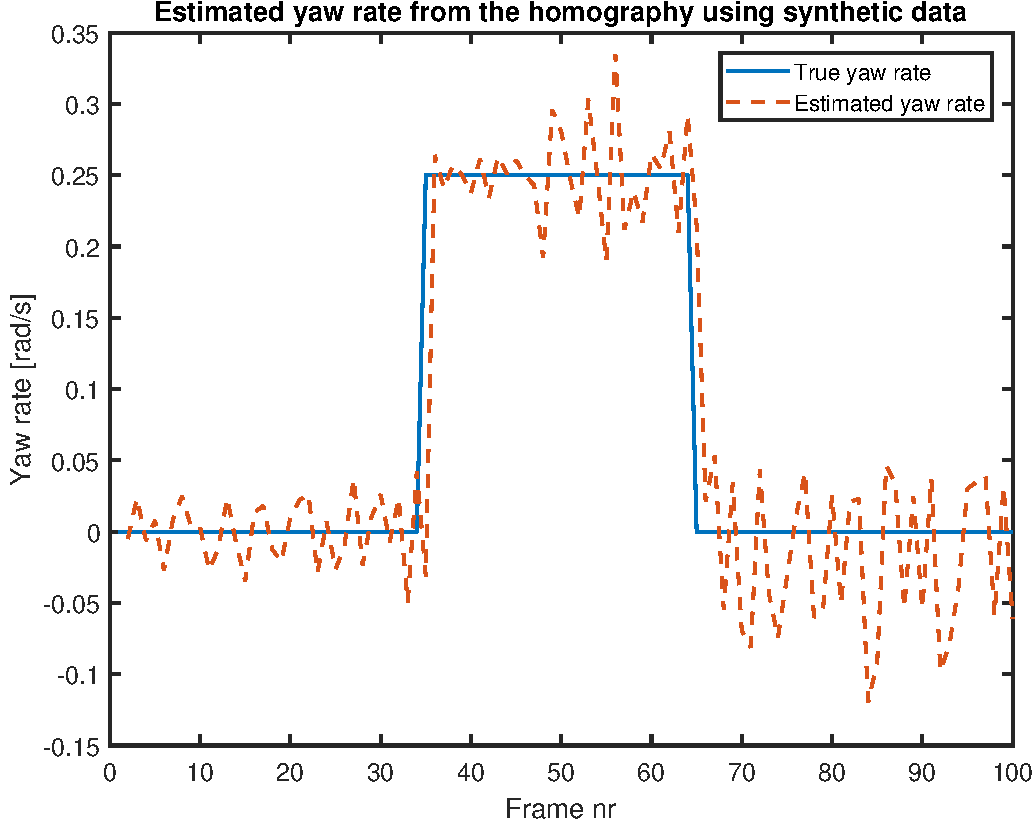
\includegraphics[width=0.7\textwidth]{RectangleSim/rect_1e-2}
	\caption{\label{fig:rectsim1e-2} Simulation result with synthetic data from a travelling rectangle. Here, Gaussian noise with a standard deviation of 0.01 pixels were added when the points on the rectangle were projected into the image plane.}
\end{figure}

\begin{figure}[!ht]
	\centering
	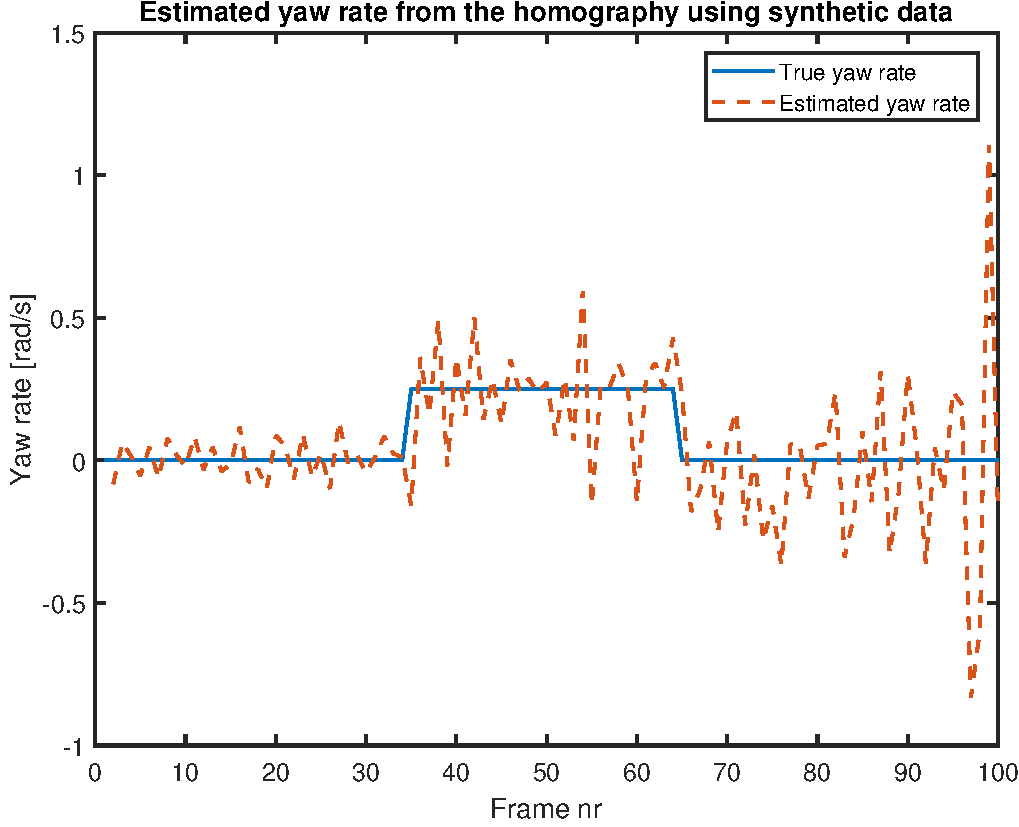
\includegraphics[width=0.7\textwidth]{RectangleSim/rect_5e-2}
	\caption{\label{fig:rectsim5e-2} Simulation result with synthetic data from a travelling rectangle. Here, Gaussian noise with a standard deviation of 0.05 pixels were added when the points on the rectangle were projected into the image plane.}
\end{figure}

\begin{figure}[!ht]
	\centering
	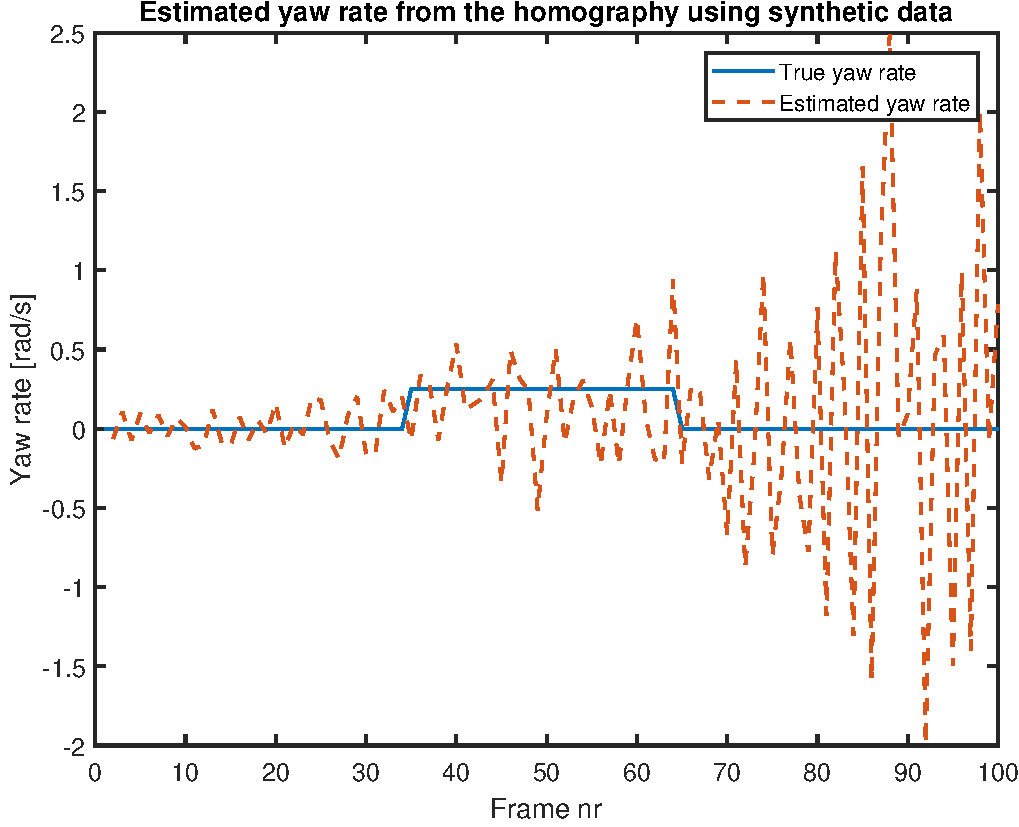
\includegraphics[width=0.7\textwidth]{RectangleSim/rect_1e-1}
	\caption{\label{fig:rectsim1e-1} Simulation result with synthetic data from a travelling rectangle. Here, Gaussian noise with a standard deviation of 0.1 pixels were added when the points on the rectangle were projected into the image plane.}
\end{figure}

\begin{figure}[!ht]
	\centering
	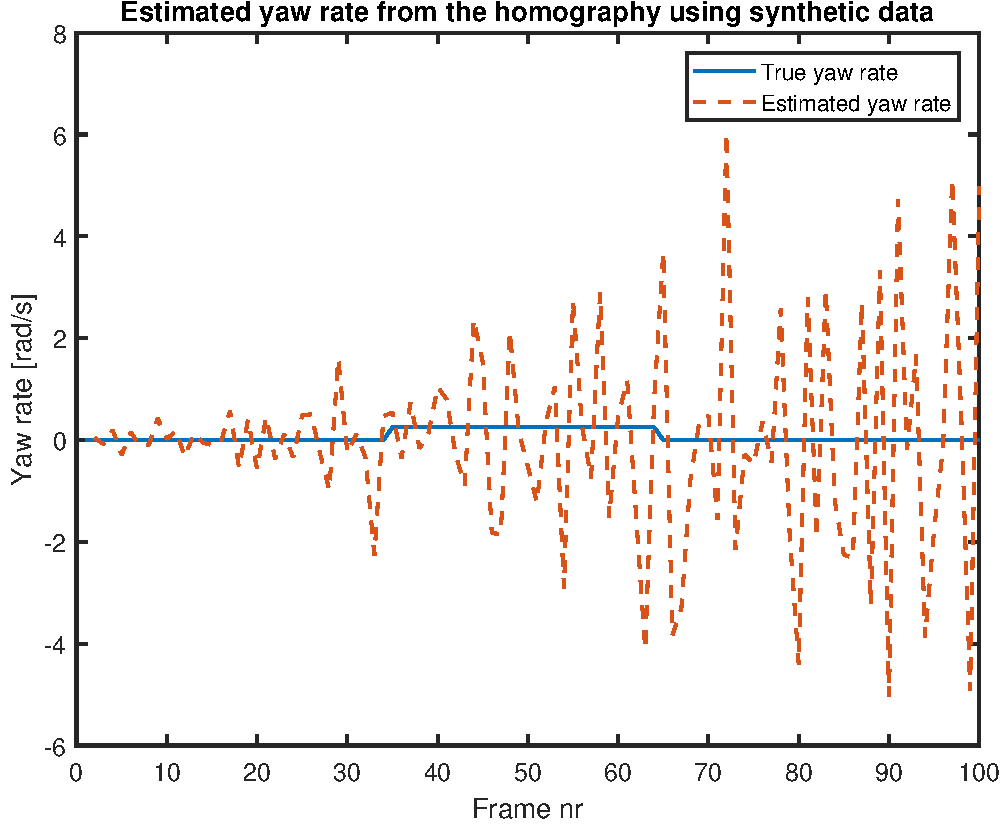
\includegraphics[width=0.7\textwidth]{RectangleSim/rect_5e-1}
	\caption{\label{fig:rectsim5e-1} Simulation result with synthetic data from a travelling rectangle. Here, Gaussian noise with a standard deviation of 0.5 pixels were added when the points on the rectangle were projected into the image plane.}
\end{figure}

\begin{figure}[!ht]
	\centering
	\subfloat[][Constructed angular rate measurements for the first sequence.]
	{
		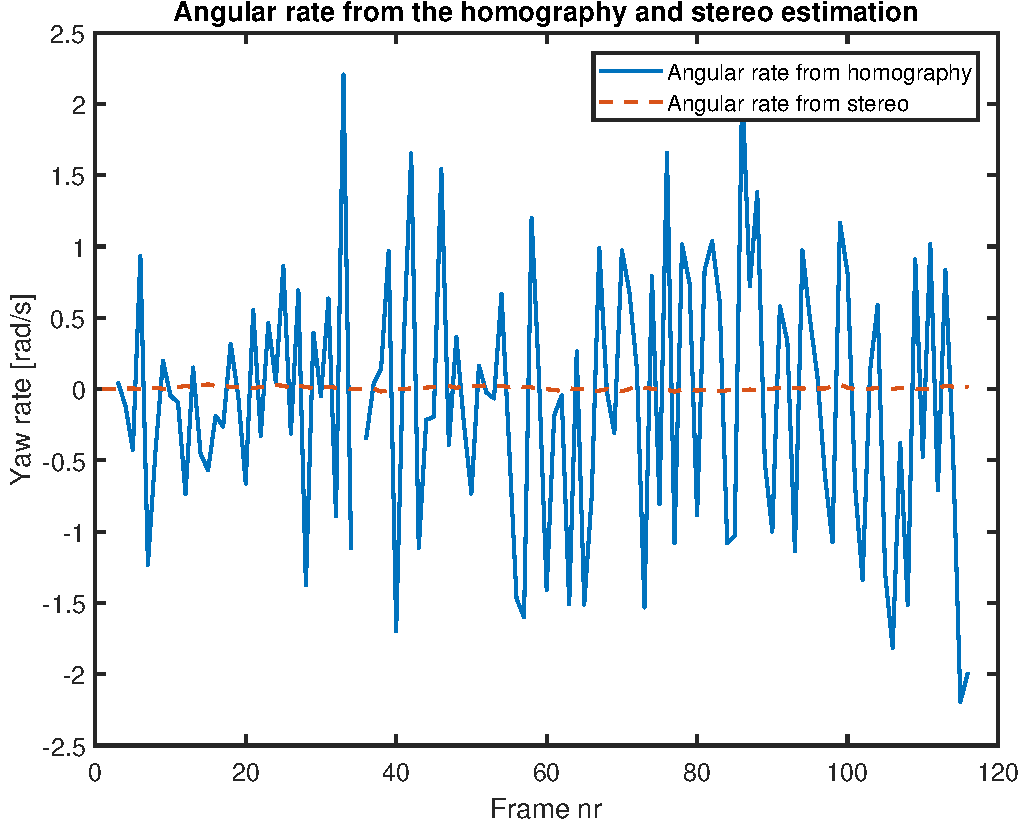
\includegraphics[width=0.7\textwidth]{StereoComparison/155532_AngVelComparison}
		\label{fig:angvelmeas155532}
	}

	\subfloat[][Constructed angular rate measurements for the second sequence.]
	{
		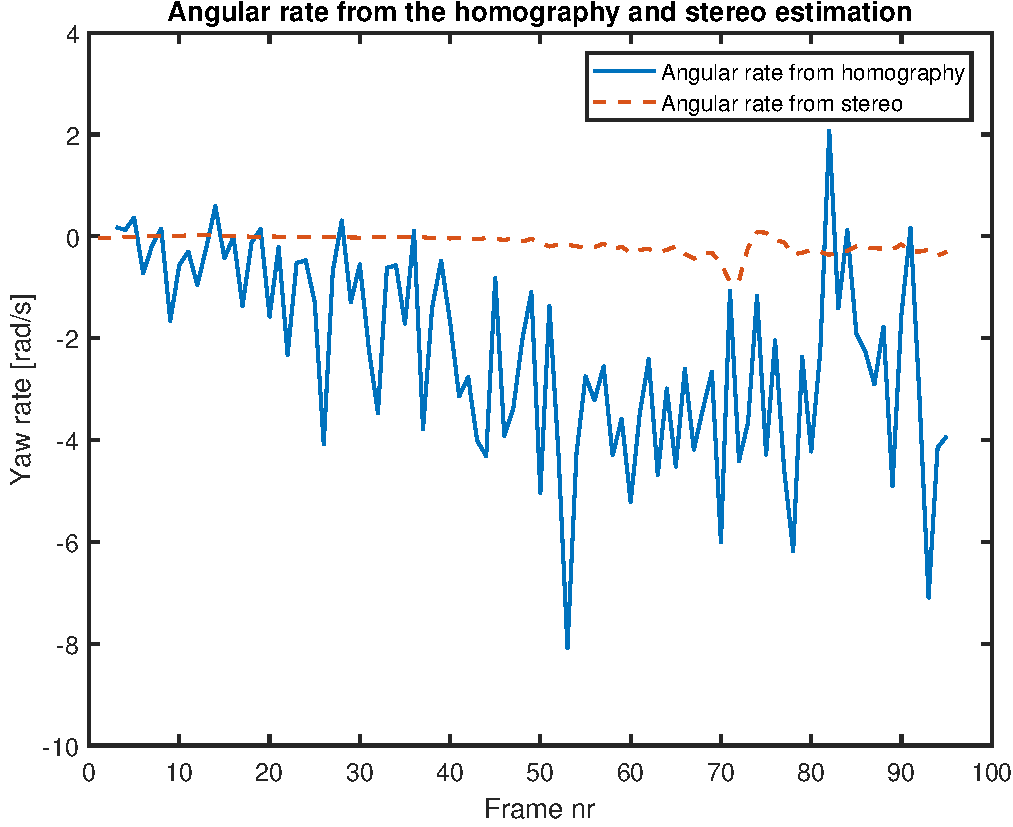
\includegraphics[width=0.7\textwidth]{StereoComparison/155733_AngVelComparison}
		\label{fig:angvelmeas155733}
	}
	\caption{\label{fig:angvelmeas} Angular rate measurements constructed from homography estimations. As a comparison, the estimated angular rate from a stereo camera system is shown as well.}
\end{figure}

\clearpage

\section{Comparison with a Stereo Camera System}
One of the goals with this \ms was to evaluate the performance of the mono tracker constructed in this thesis with a stereo system.
For this purpose, real-world data were collected with a stereo camera system to use as ''ground truth''.
The two sequences, which a comparison has been performed with, are shown in \Figureref{fig:sequence155532} and \Figureref{fig:sequence155733}.
The first sequence contains a target which travels straight forward and the second sequence contains a target which makes a turn to the right.

The resulting state comparisons are presented in \Figureref{fig:comparison155532} and \Figureref{fig:comparison155733}.
The estimated states from the stereo camera had poor performance in some parts of the sequence.
In the first sequence, the poor stereo states estimates in $x$ and $\psi$ around frame number 100 gave a large error in the comparison.
In the second sequence, the poor stereo states estimates in $v$ and $\omega$ around frame number 72 gave a large error in the comparison.

When the target is travelling straight, there is less performance to gain by adding the corners as measurements compared to just using the \abbrROI and angular rate as measurements.
Compare \Figureref{fig:roiangvel155532} with \Figureref{fig:roicorner155532} and \Figureref{fig:all155532}.
This might depend on that the generated angular rate measurements were better for this particular scenario, see \Figureref{fig:angvelmeas155532}, than for the turning scenario in \Figureref{fig:angvelmeas155733}.

By looking in \Figureref{fig:angvelmeas155733}, one can see that the angular rate measurements overestimates the turning rate.
Therefore, the filter was tuned with a high variance for the angular rate measurement in the measurement noise covariance matrix $\bm{R}$.
In this sequence, the state estimate gets improved by substituting the angular rate for corner measurements.
Compare \Figureref{fig:roiangvel155733} with \Figureref{fig:roicorner155733} and especially note the improvement of the yaw angle towards the end of the sequence.
From frame number 60, three corners of the target were visible which improved the orientation estimation.
When all three measurements are combined, in \Figureref{fig:all155733}, a similar result to \Figureref{fig:roicorner155733} is obtained.

\begin{figure}[!ht]
	\centering
	\subfloat[][Frame number 1.]
	{
		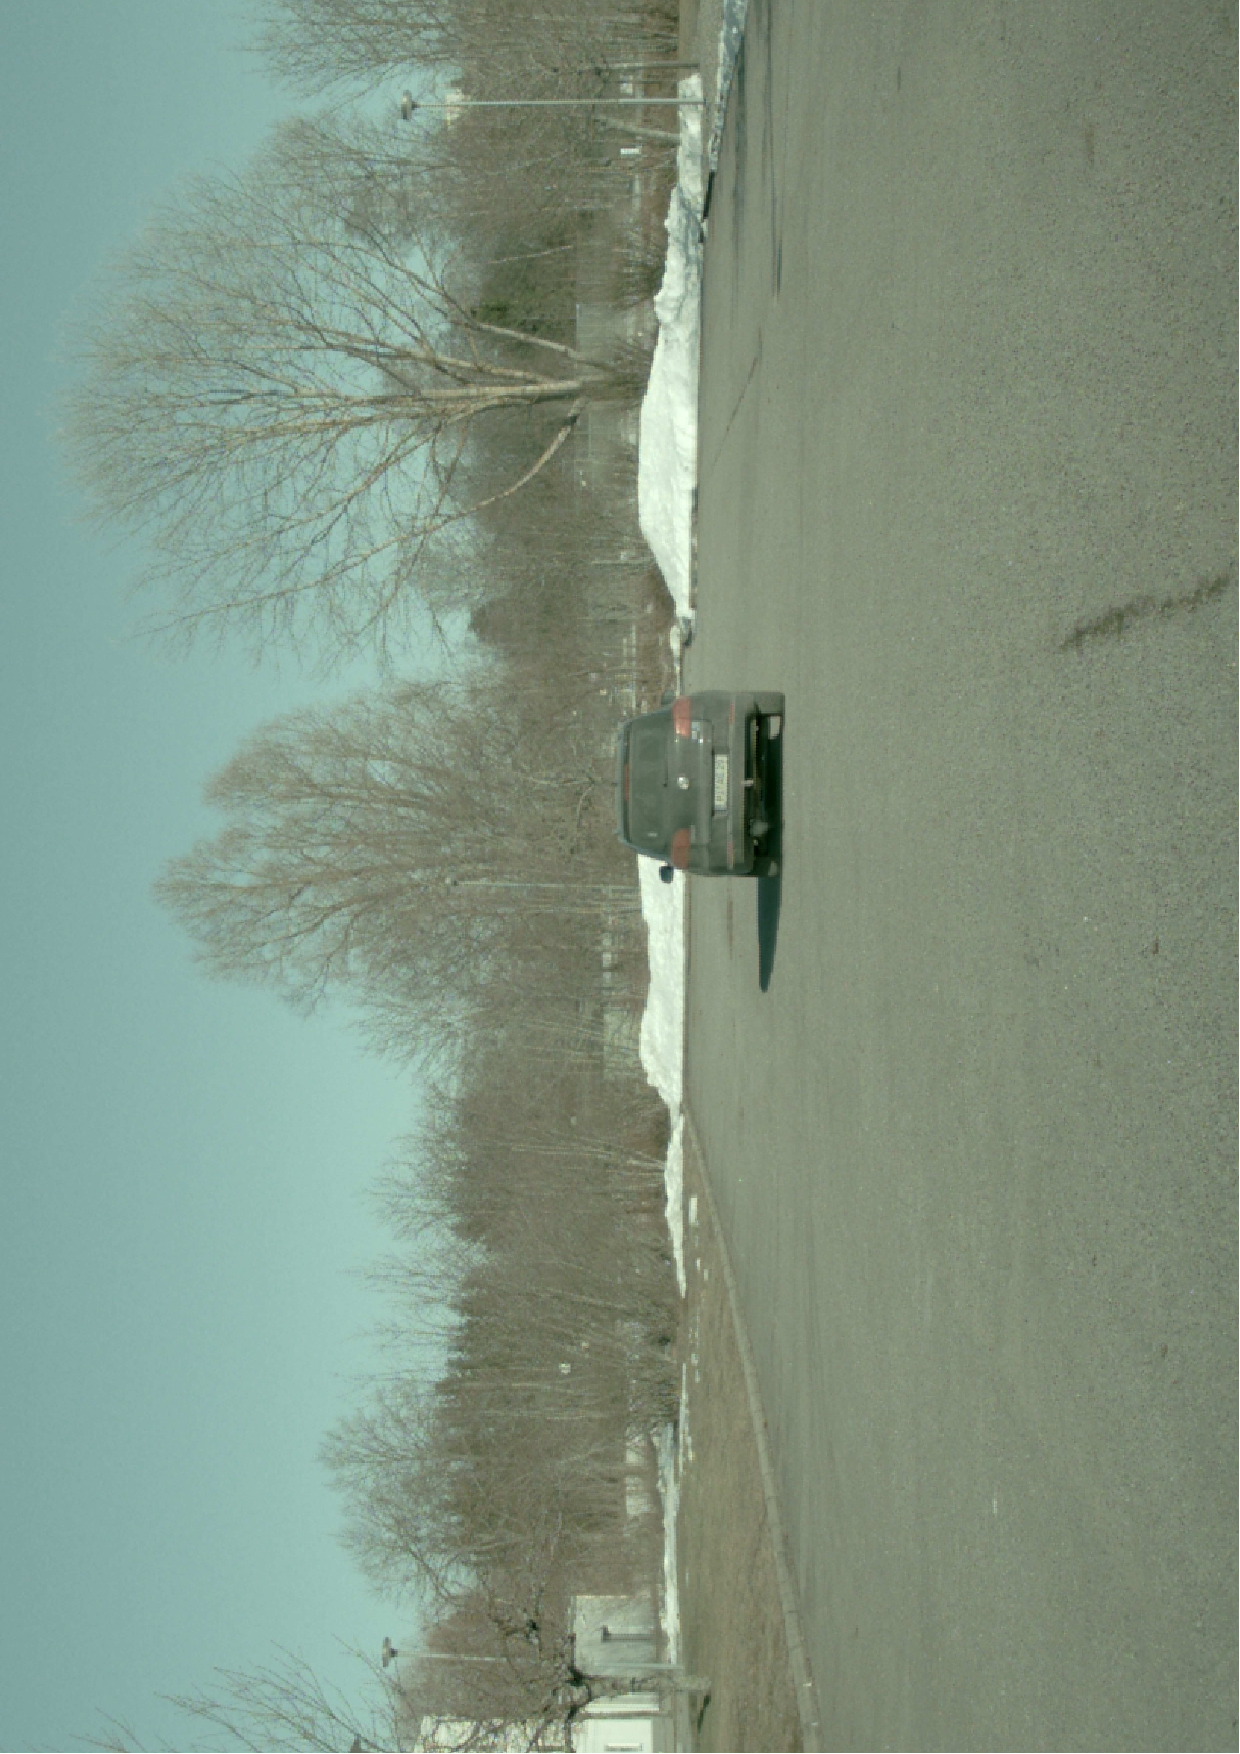
\includegraphics[angle=-90,origin=c,trim={0 0 5cm 0},width=0.55\textwidth]{Sequences/155532_1}
		\label{fig:155532_1}
	}

	\subfloat[][Frame number 45.]
	{
		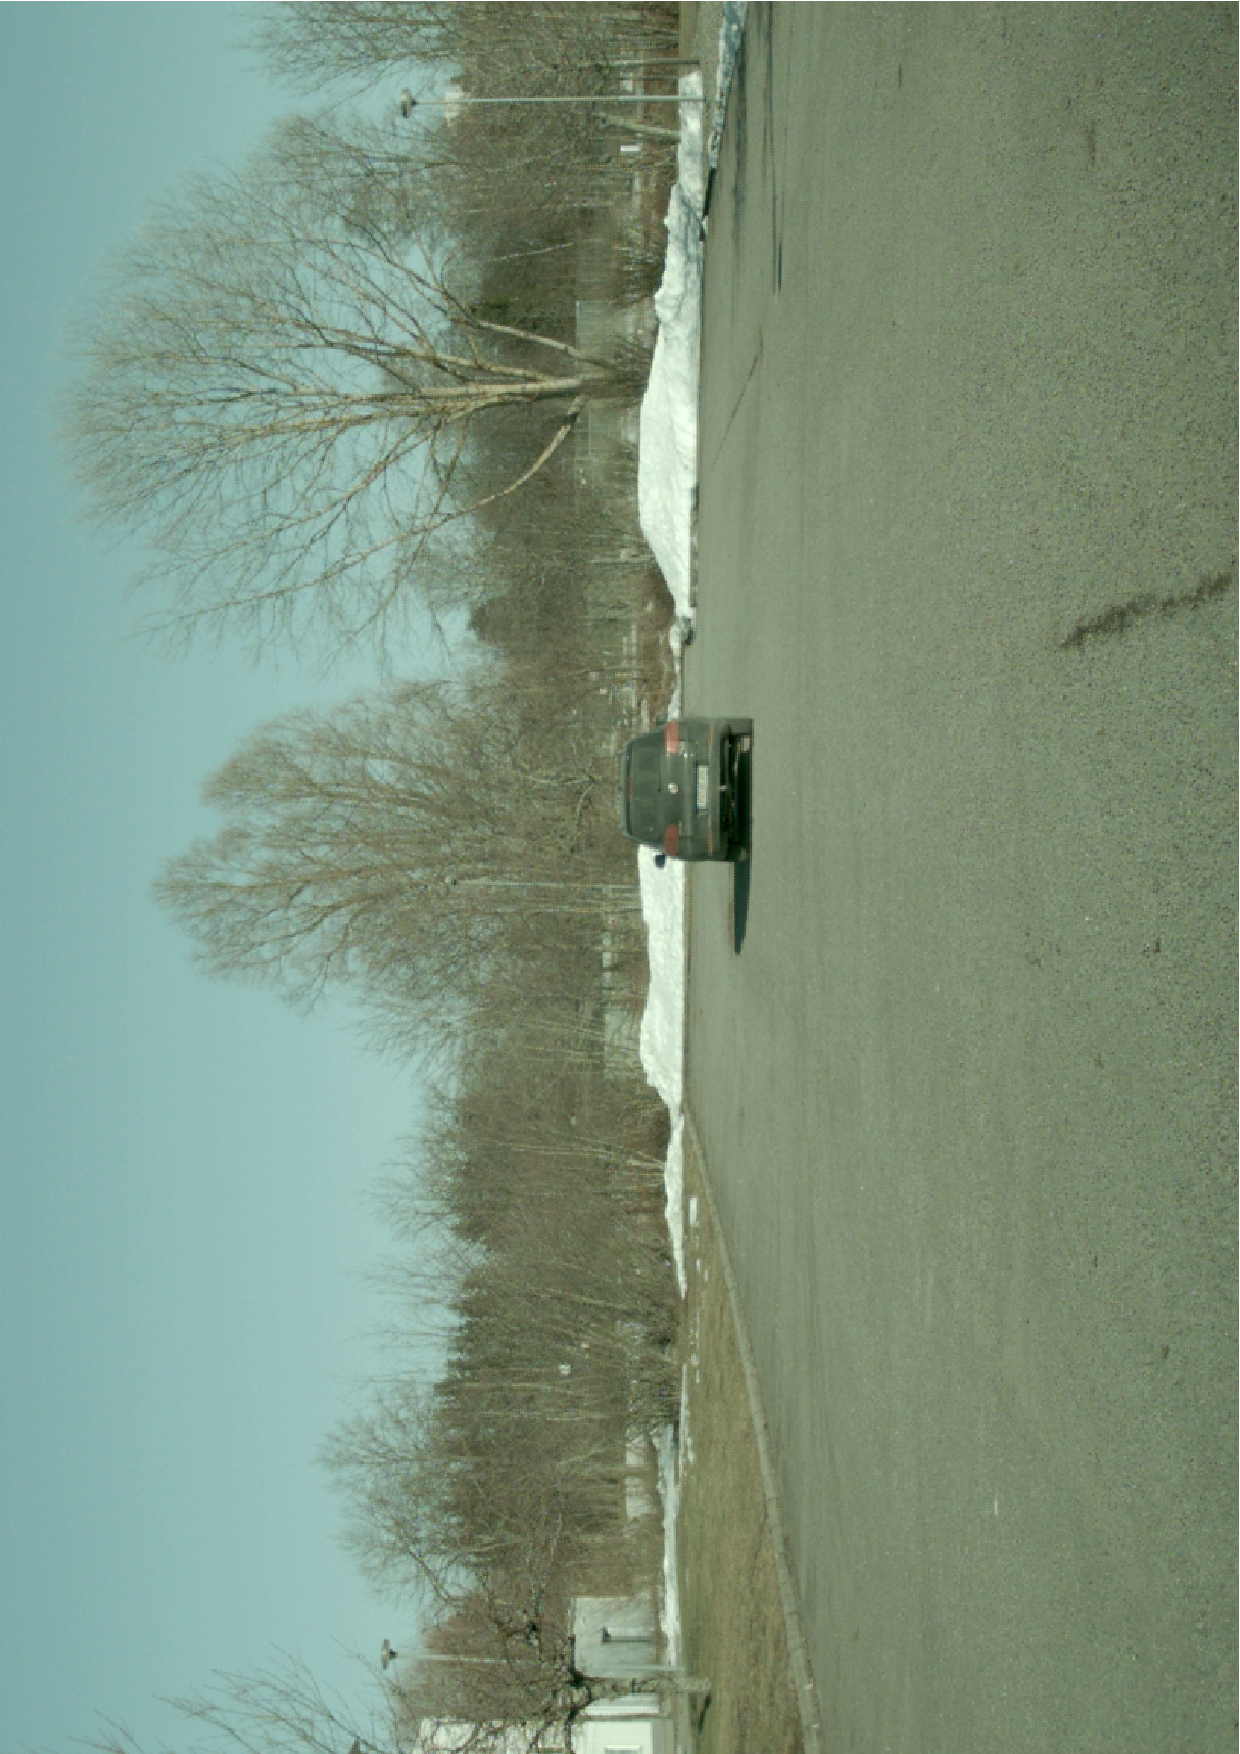
\includegraphics[angle=-90,origin=c,trim={0 0 5cm 0},width=0.55\textwidth]{Sequences/155532_45}
		\label{fig:155532_45}
	}

	\subfloat[][Frame number 95.]
	{
		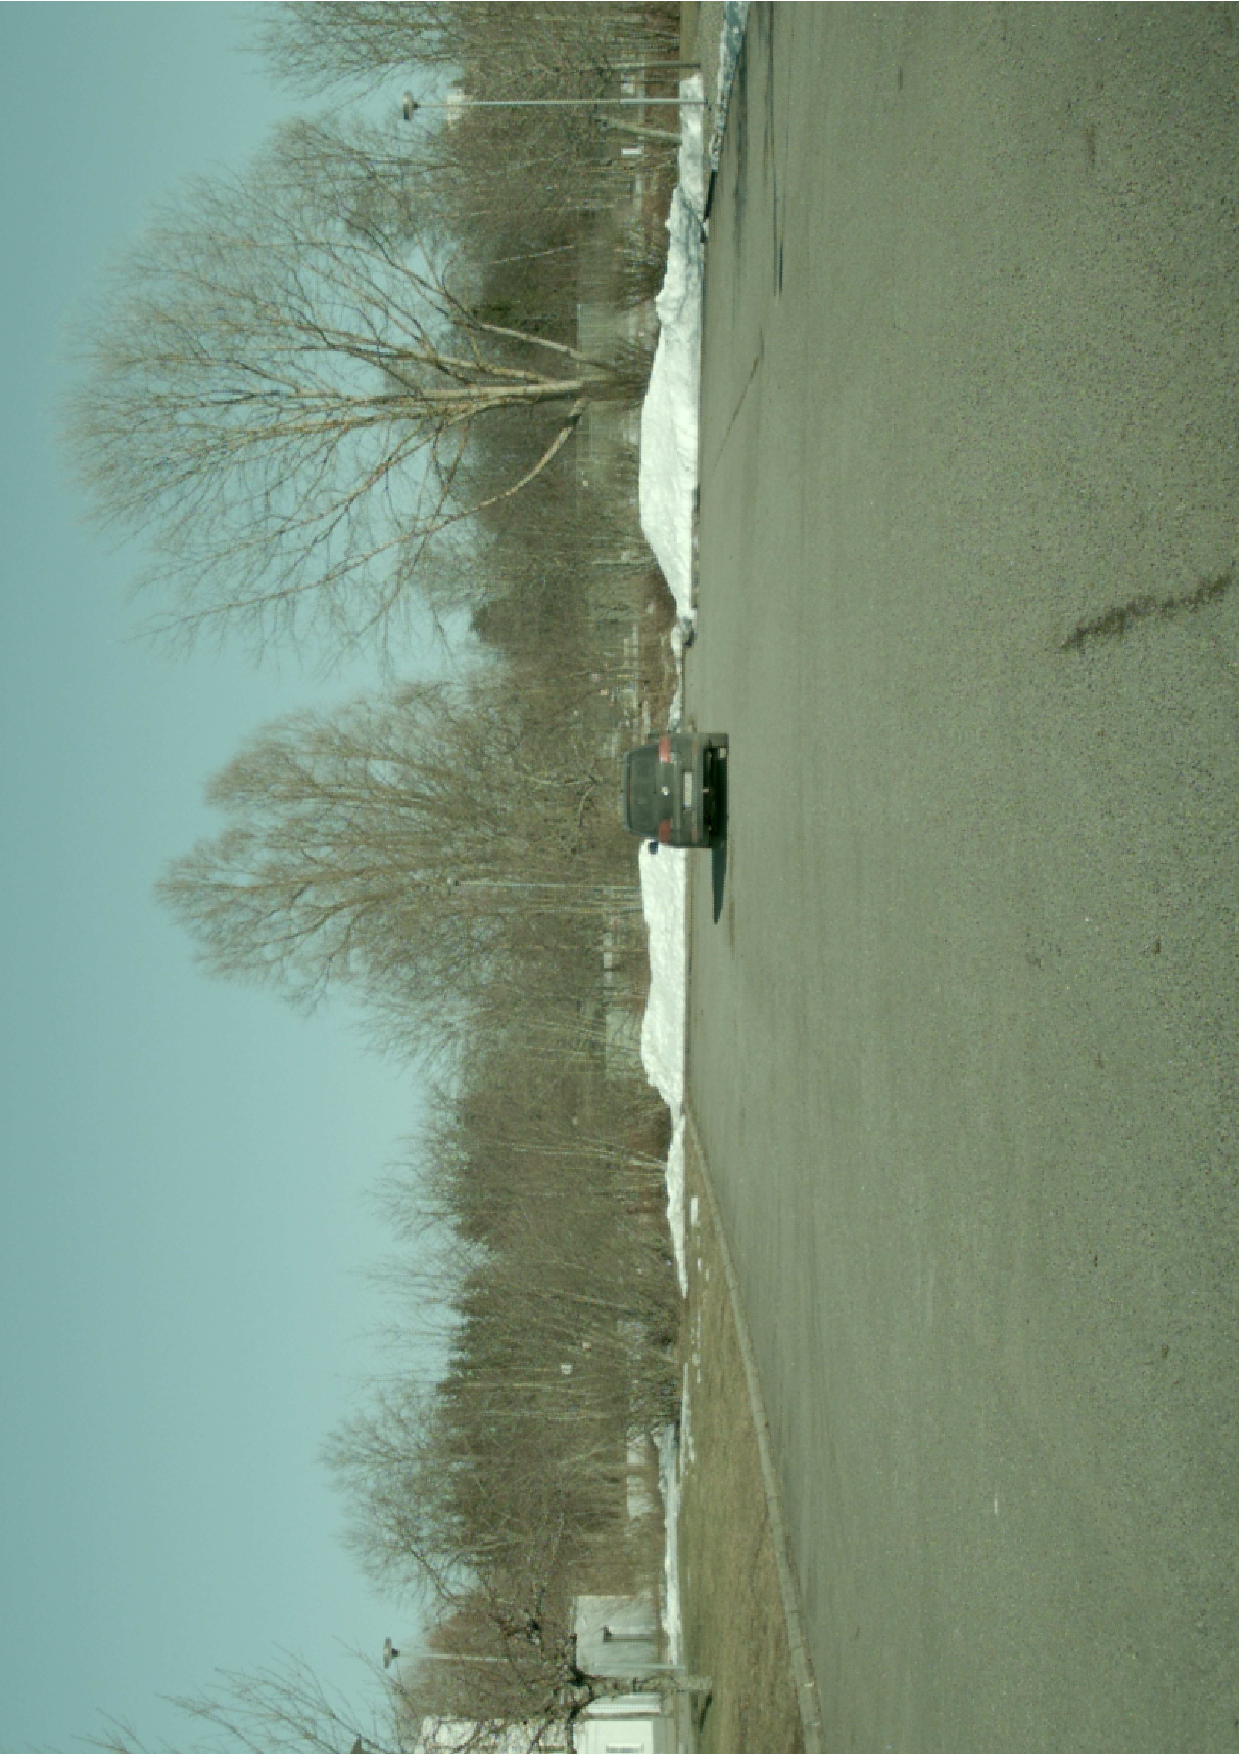
\includegraphics[angle=-90,origin=c,trim={0 0 5cm 0},width=0.55\textwidth]{Sequences/155532_95}
		\label{fig:155532_95}
	}
	\caption{\label{fig:sequence155532} The first sequence where the target vehicle drives straight forward, away from the host.}
\end{figure}

\begin{figure}[!ht]
	\centering
	\subfloat[][Frame number 20.]
	{
		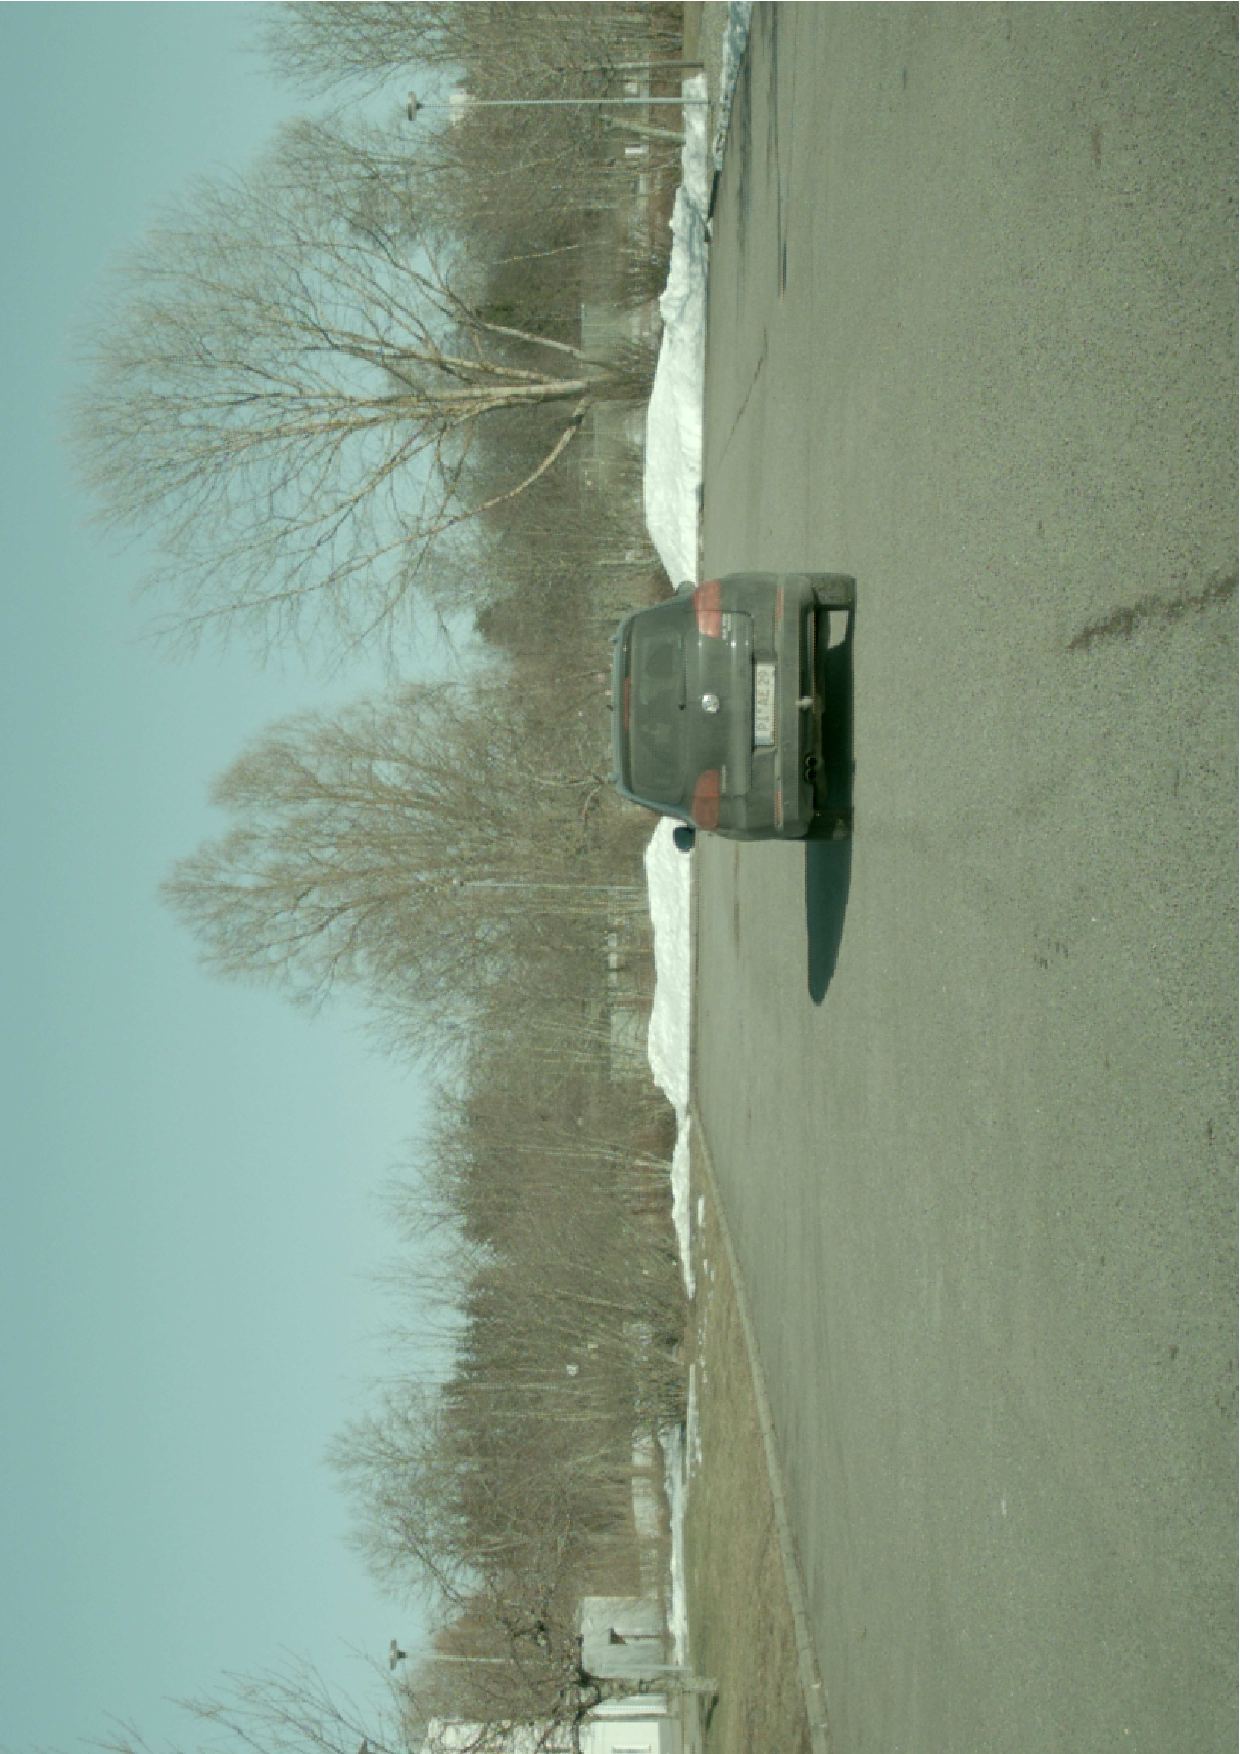
\includegraphics[angle=-90,origin=c,trim={0 0 5cm 0},width=0.55\textwidth]{Sequences/155733_20}
		\label{fig:155733_20}
	}

	\subfloat[][Frame number 55.]
	{
		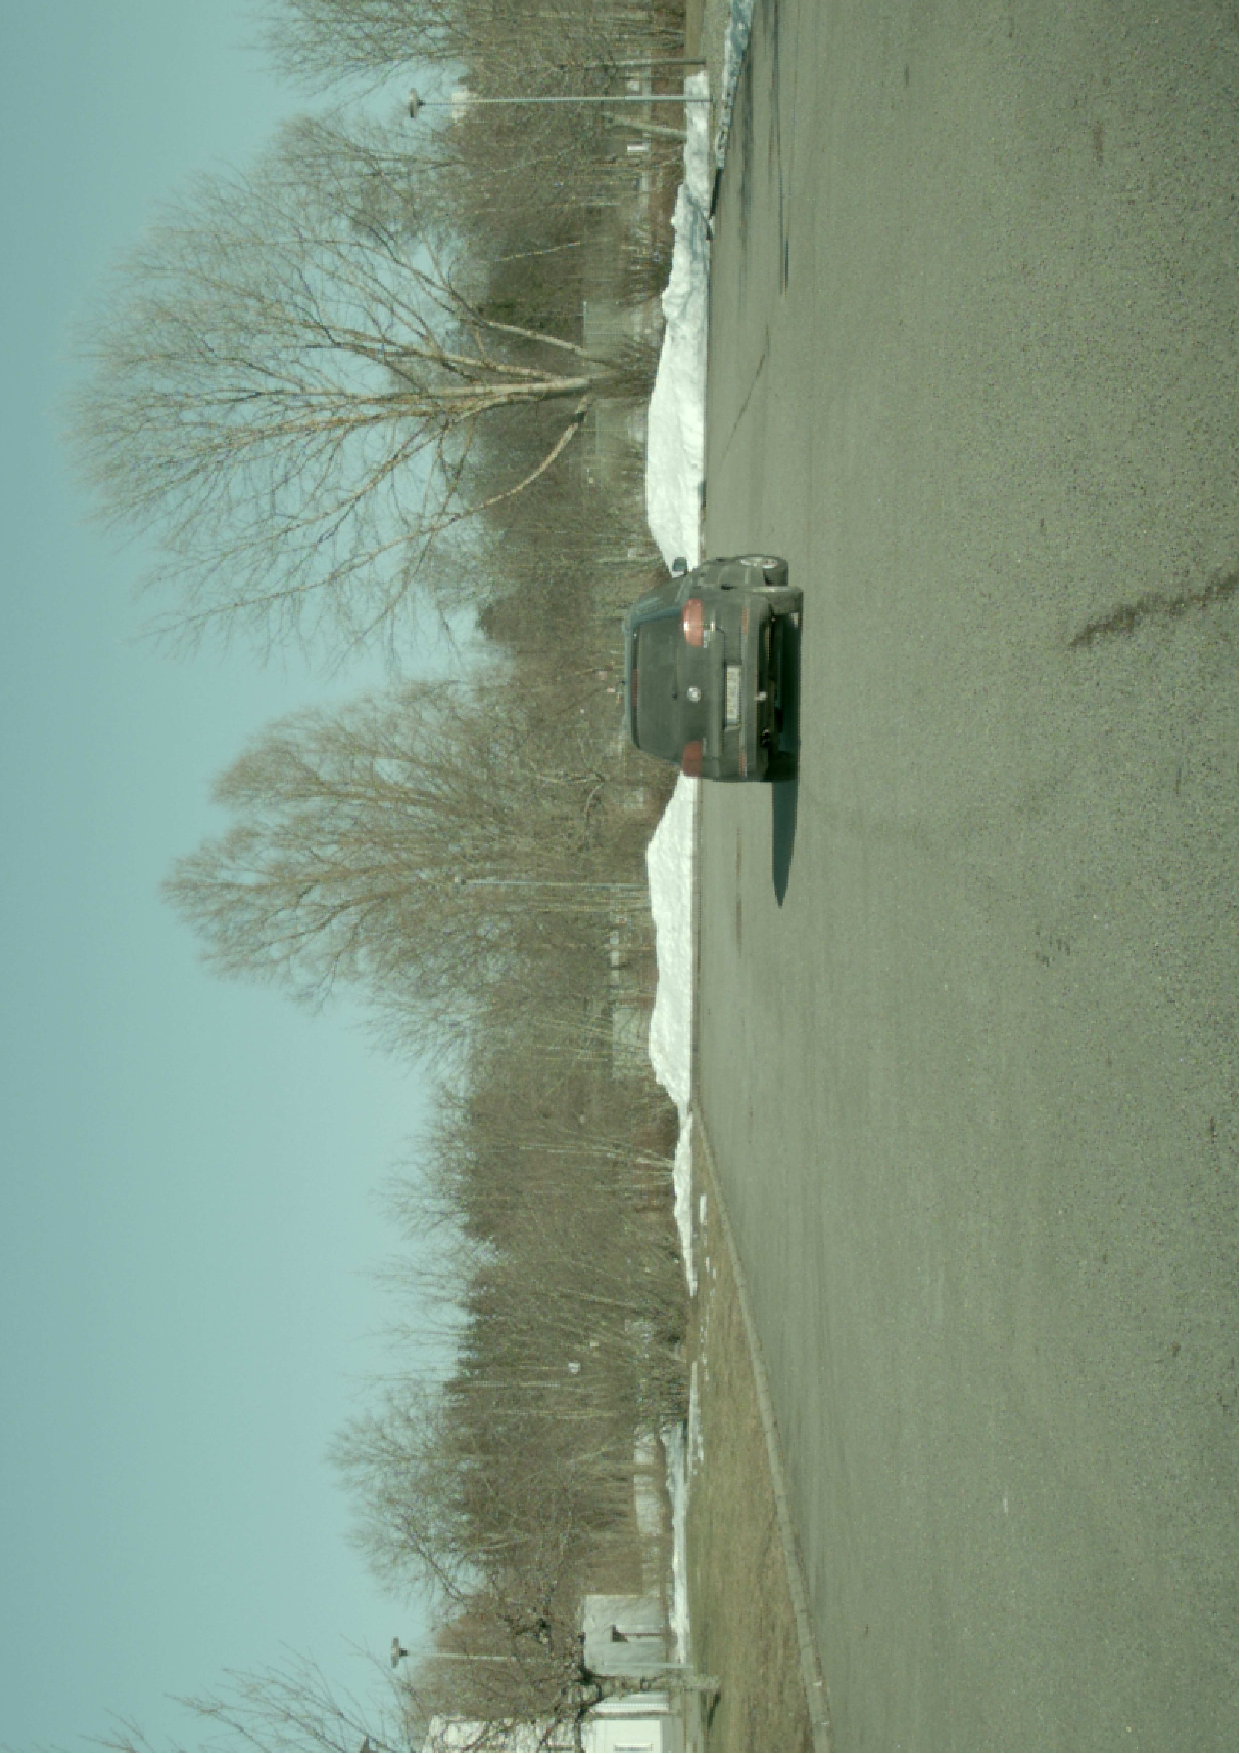
\includegraphics[angle=-90,origin=c,trim={0 0 5cm 0},width=0.55\textwidth]{Sequences/155733_55}
		\label{fig:155733_55}
	}

	\subfloat[][Frame number 95.]
	{
		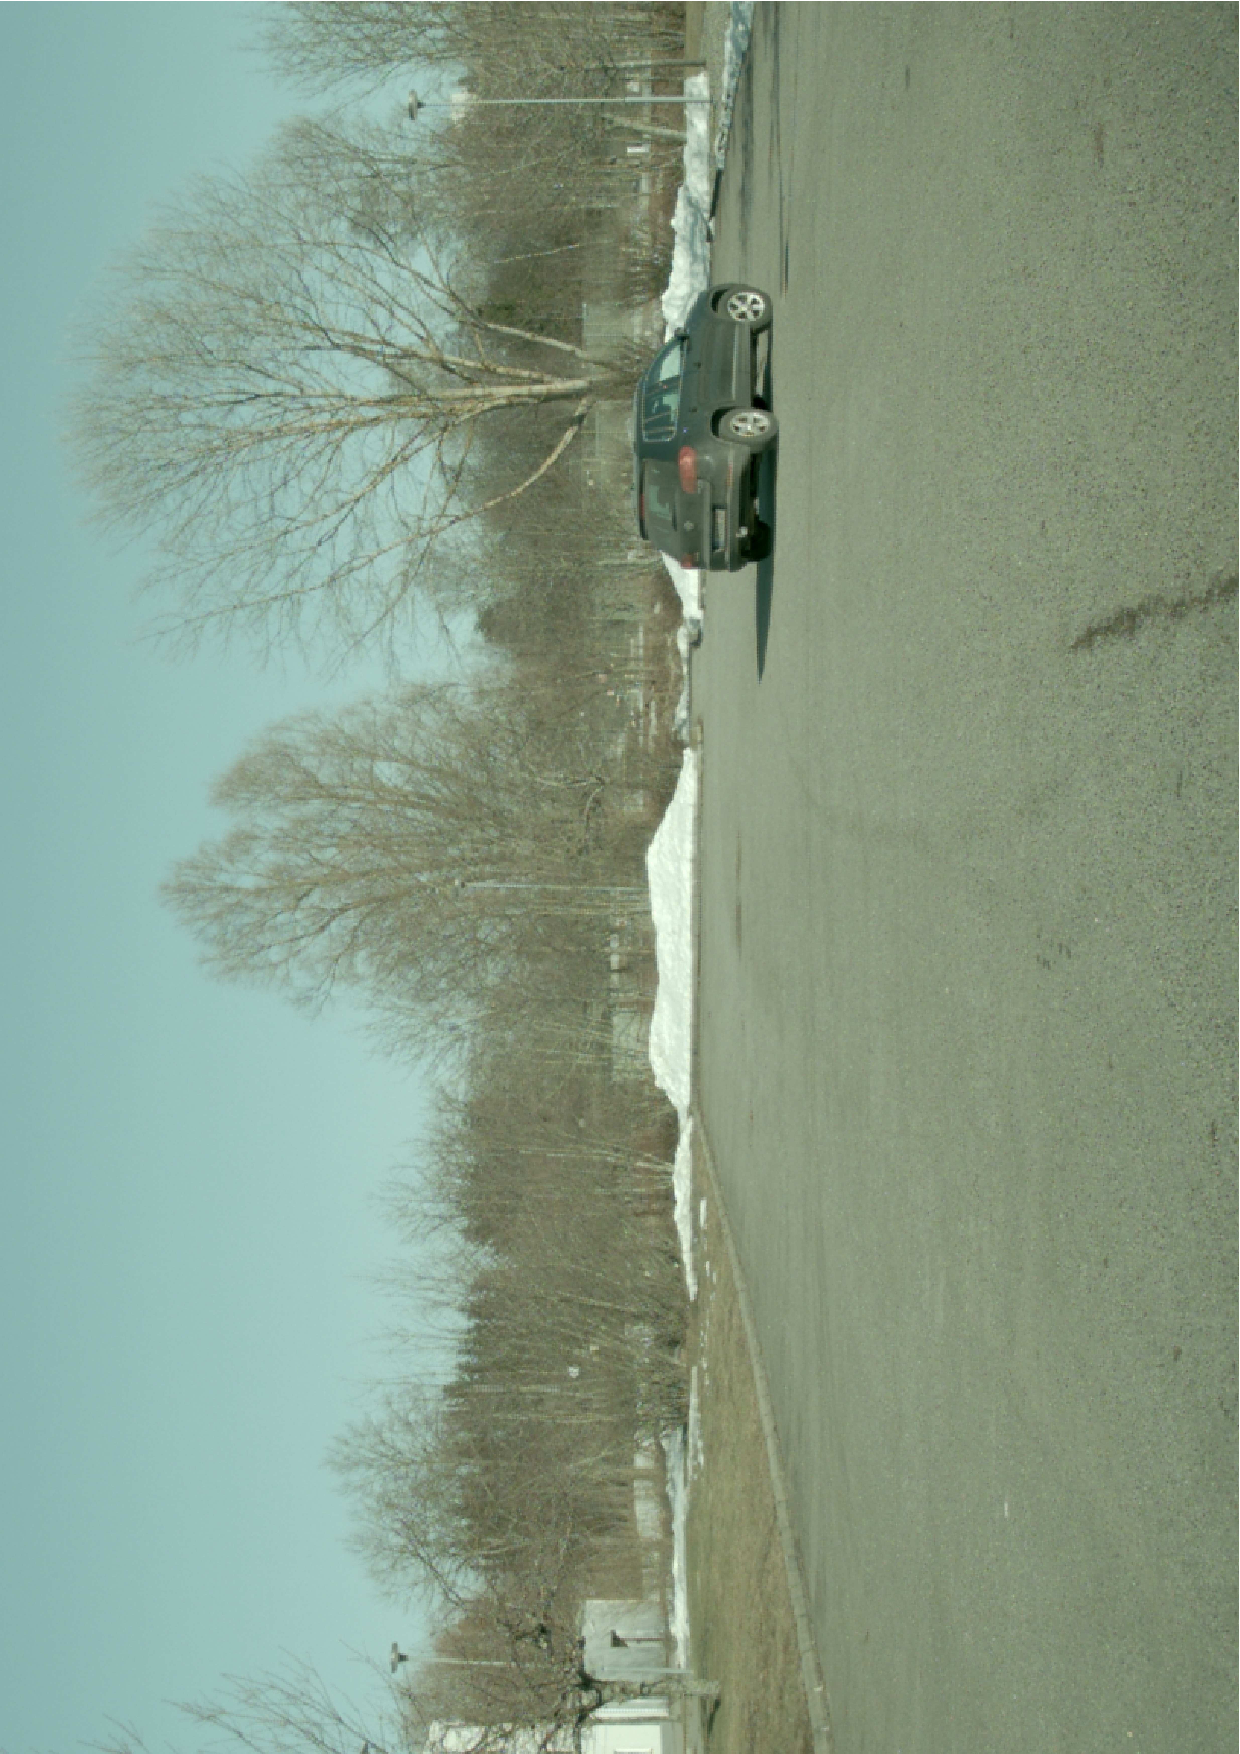
\includegraphics[angle=-90,origin=c,trim={0 0 5cm 0},width=0.55\textwidth]{Sequences/155733_95}
		\label{fig:155733_95}
	}
	\caption{\label{fig:sequence155733} The second sequence where the target vehicle drives straight and then turns to the right.}
\end{figure}

\begin{figure}[!ht]
	\centering
	\subfloat[][Comparison with a stereo camera system, using \abbrROI and angular rate as measurements in the mono camera system.]
	{
		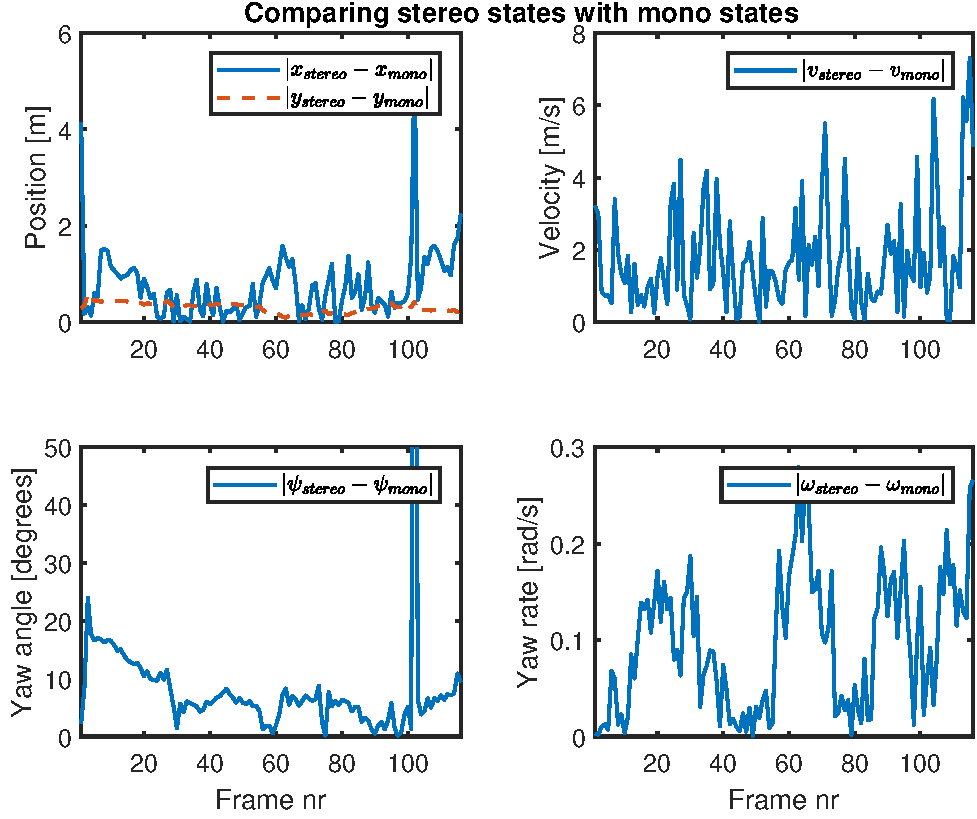
\includegraphics[width=0.7\textwidth]{StereoComparison/155532_RoiAngVel_gate_klt}
		\label{fig:roiangvel155532}
	}

	\subfloat[][Comparison with a stereo camera system, using \abbrROI and corners as measurements in the mono camera system.]
	{
		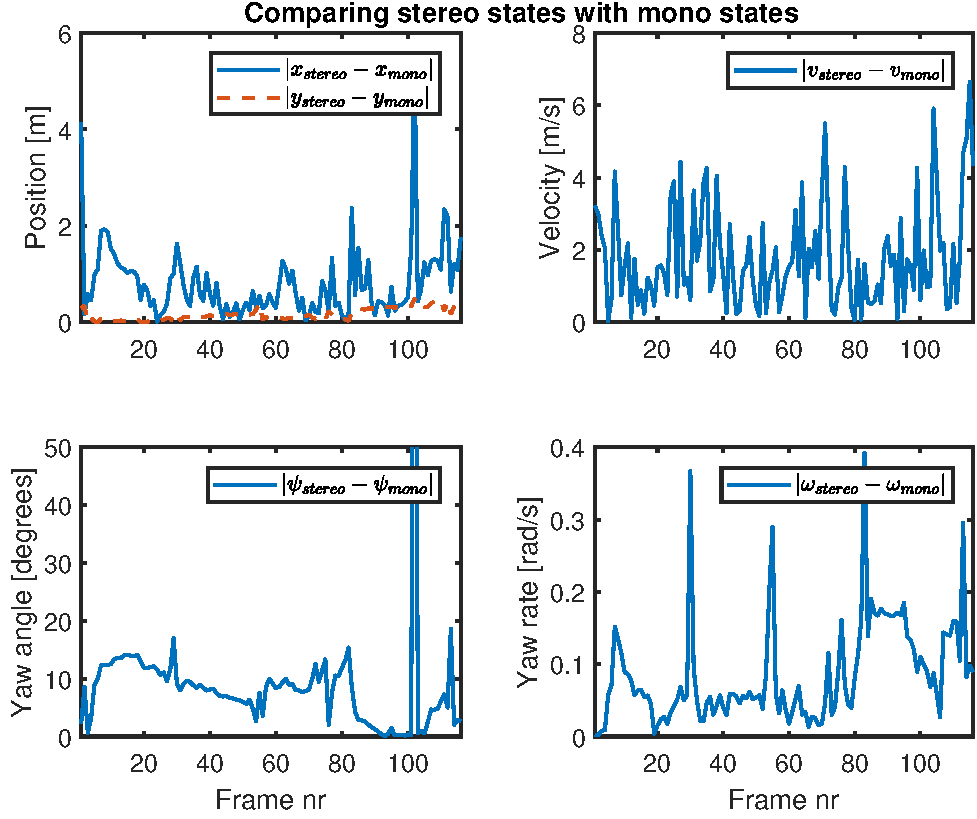
\includegraphics[width=0.7\textwidth]{StereoComparison/155532_RoiCorner_gate_klt}
		\label{fig:roicorner155532}
	}
	\caption{Comparison with a stereo camera system for the first sequence.}
\end{figure}

\begin{figure}[!ht]
	\centering
	\ContinuedFloat
	\subfloat[][Comparison with a stereo camera system, using all three measurements in the mono camera system.]
	{
		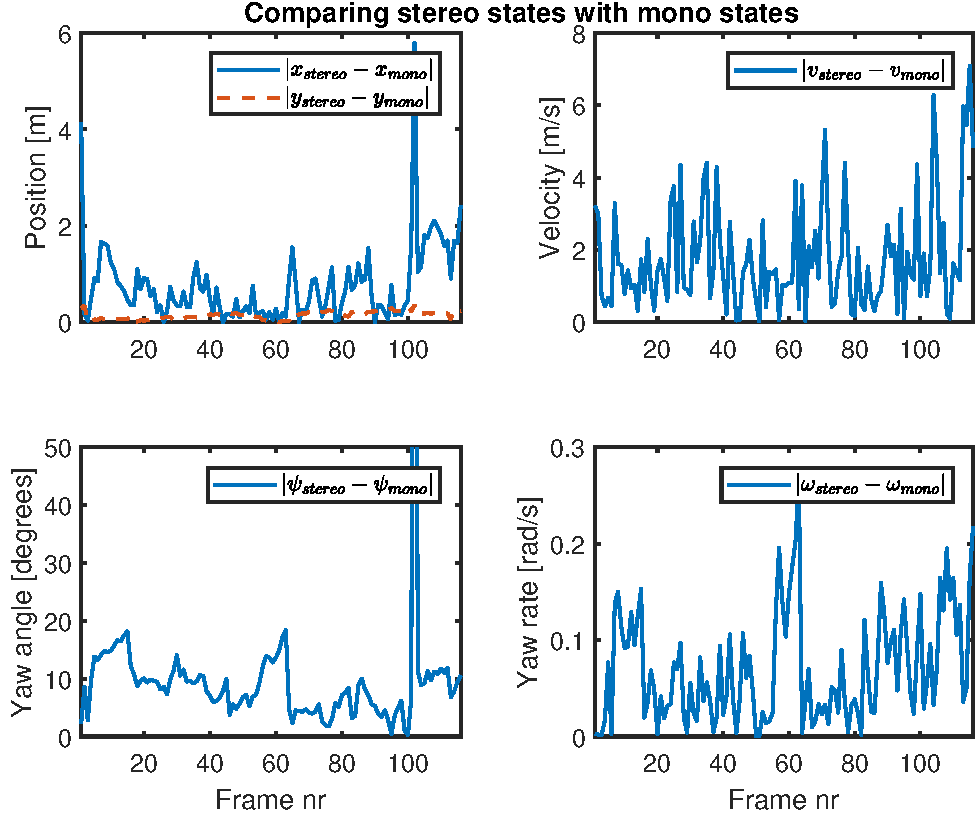
\includegraphics[width=0.7\textwidth]{StereoComparison/155532_AllMeasurements_gate_klt}
		\label{fig:all155532}
	}
	\caption{\label{fig:comparison155532} Comparison with a stereo camera system for the first sequence.}
\end{figure}

\begin{figure}[!ht]
	\centering
	\subfloat[][Comparison with a stereo camera system, using \abbrROI and angular rate as measurements in the mono camera system.]
	{
		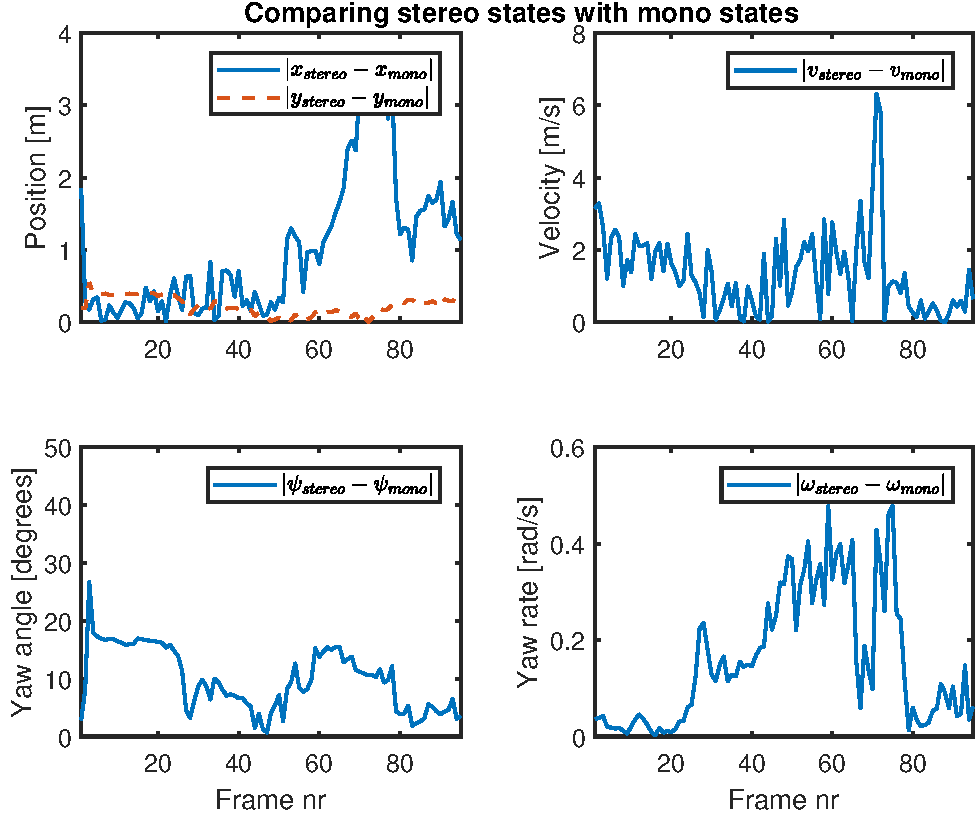
\includegraphics[width=0.7\textwidth]{StereoComparison/155733_RoiAngVel_gate_klt}
		\label{fig:roiangvel155733}
	}
	\caption{Comparison with a stereo camera system for the second sequence.}
\end{figure}

\begin{figure}[!ht]
	\centering
	\ContinuedFloat
	\subfloat[][Comparison with a stereo camera system, using \abbrROI and corners as measurements in the mono camera system.]
	{
		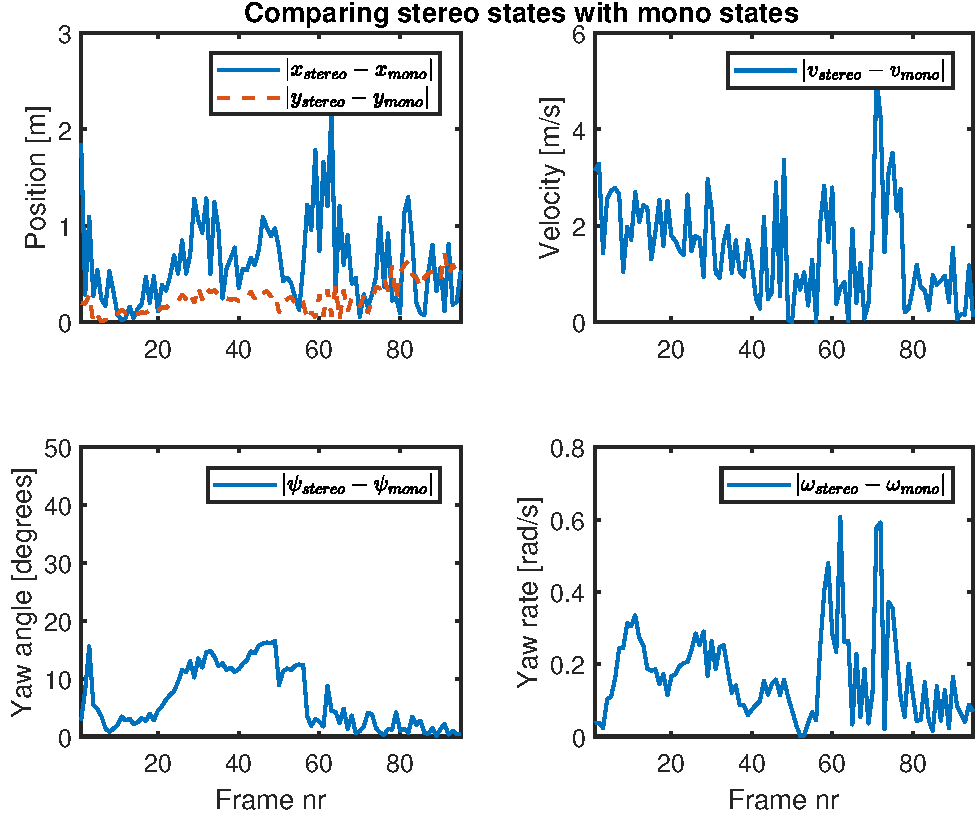
\includegraphics[width=0.7\textwidth]{StereoComparison/155733_RoiCorner_gate_klt_perf}
		\label{fig:roicorner155733}
	}

	\subfloat[][Comparison with a stereo camera system, using all three measurements in the mono camera system.]
	{
		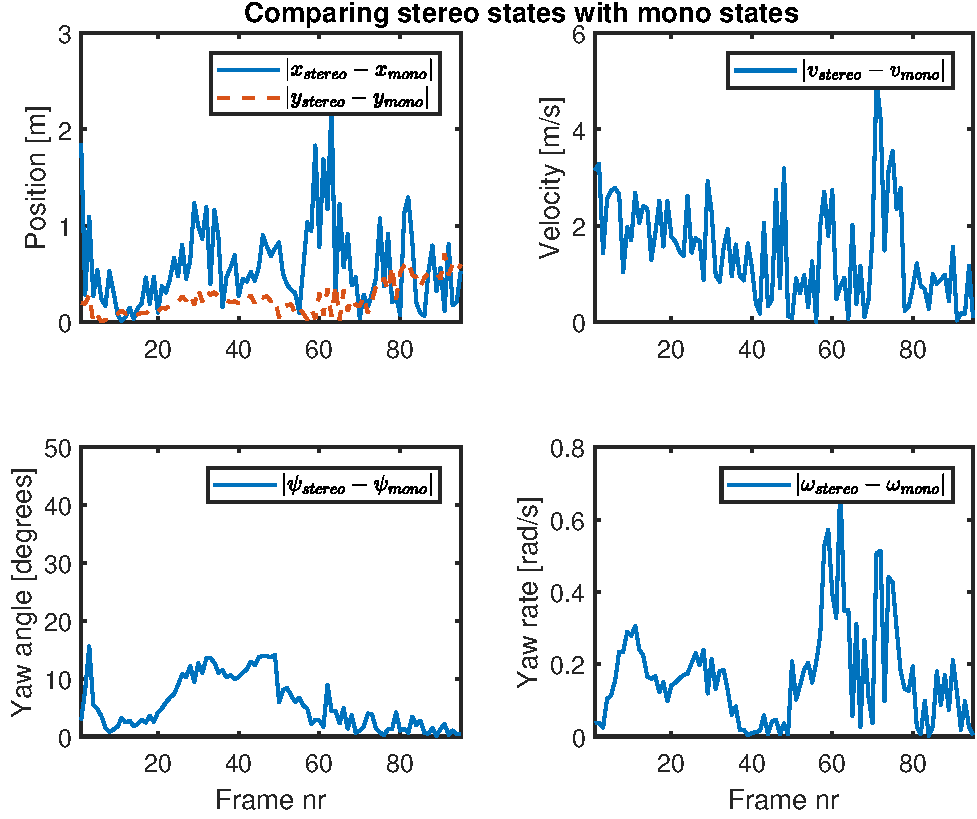
\includegraphics[width=0.7\textwidth]{StereoComparison/155733_AllMeasurements_gate_klt_perf}
		\label{fig:all155733}
	}
	\caption{\label{fig:comparison155733} Comparison with a stereo camera system for the second sequence.}
\end{figure}
\chapter{Conclusions and Future Work}
\label{cha:conclusions}

This thesis has shown that it is possible to estimate the heading (orientation and angular rate) of a vehicle using a mono camera system.
There is still some continued work that has to be done in order to achieve the same level of performance as a stereo camera system.

\section{Conclusions}
Through this thesis, a proposed model has been presented in order to solve the heading estimation problem.
Given the results presented in this thesis and the related research described in \Sectionref{sec:relatedresearch}, the thesis has shown that it is possible to estimate the heading of a vehicle using a mono camera system.
This thesis has shown, through Monte Carlo simulations, that given the proper measurements and measurements with plausible noise variance level, the proposed method is able to estimate the orientation and angular rate of a target vehicle.
The modelling strategy, by modelling the target as a rectangle, seems like a suitable model for describing the target.
It captures the shape of the target in a good way and the rotation is easily defined in the model.
The model is also suitable for measurements of the target vehicle's corners.
Although no other models have been tested in this thesis, the rectangle model seems like an eminent model choice.

The results with real-world data were not as satisfying as the best simulated results.
Due to the high variance of the constructed angular rate measurements, the same gratifying results achieved through simulations could not be obtained with real-world data.
By adding the target vehicle's corners as measurements, the state estimates could further be improved in the case of a turning target.

\newpage

By recalling the objective of this thesis including the questions that were stated in \Chapterref{cha:intro}, answers can now be provided in order to finalize the thesis.

\begin{itemize}
    \item Can the heading of a vehicle be estimated using a mono camera system?

    Yes, the heading of a vehicle can be estimated using a mono camera system if the proper measurements are available with high enough reliability.

    \item What kind of algorithms and models are suitable for solving the problem?

    By modelling the target vehicle as a rectangle and using the proposed measurements, a suitable algorithm has been constructed in order to solve the heading estimation problem.

    \item How well does the estimates from a mono camera system perform compared to those from a stereo camera system?

    From the results in this thesis, the mono camera system can not quite catch up with the performance of a stereo camera system.
    The result could be improved by
	\begin{enumerate}[label=\roman*)]
		\item increasing the number of feature points or improve the feature point correspondence between two frames,
		\item further investigate the homography estimation method,
		\item constructing a method which can generate measurements of the corners.
	\end{enumerate}
	If these improvements are implemented, then the mono camera system can have a reasonable chance of competing in performance with a stereo camera system.
\end{itemize}

\section{Suggestions for Future Work}
There are several things which could be improved in the future.
Right now, the mono camera system is still lacking behind in the capability of estimating the heading of vehicles, compared to a stereo camera system.
By looking at the thesis limitations, several tasks for future work can be stated.
However, a couple of more interesting future tasks are mentioned here.

\subsection{Homography Estimation}
By further investigating the homography estimation method, perhaps the noise level could be reduced.
Data normalization, \eg Hartley normalization \cite{Nordberg:2015}, is one concept which might improve the homography estimation.
Another method is to reduce the number of parameters to estimate in the homography matrix.
Since the homography describes the rotation in three dimensions it should be possible to reduce the number of free parameters.
A vehicle can (in normal cases) only rotate in one of the three dimensions.

\subsection{Feature Point Correspondence}
Testing another method for the feature point detection, description, matching and tracking might also be a strategy to obtain better homography estimations.
Since the quality of the estimated yaw rate from the homograpy did not match the quality of the estimated yaw rate in \cite{Gabb:2013}, improving the KLT feature point tracker could be one way forward.
The feature point detection could also be analysed further.
As discussed in \Sectionref{sec:homographyestimationresults}, the quality and spatial location of the detected feature points have an important role for the homography estimation.
One thing to have in mind is that in this thesis the feature point tracker where implemented in \matlab.
If it should run in a mono camera system, different aspects of the computation complexity might have to be taken into consideration.

\subsection{Corner Measurements}
This thesis has shown that corner measurements could improve the heading estimation in a mono camera system.
Coming up with a method to construct a detector, which could detect the corners in the image, could therefore be a highly interesting part of the future work.

\part*{Appendix}
\appendix
\chapter{Monte Carlo Simulations}
\label{app:montecarlo}

All Monte Carlo simulations performed in this thesis are listed in this appendix.
The Monte Carlo simulations were performed by first simulating a trajectory, using the motion model.
The model state velocity and angular velocity were also driven by Gaussian process noise in order to not simulate a perfect trajectory.
The trajectory was estimated with generated measurements plus Gaussian measurement noise in order to simulate real-world measurements.
The estimated states were then compared to the simulated states by calculating the \abbrRMSE.

Here, some additional figures to the once presented in \Chapterref{cha:result} will be shown presenting examples of the simulated and estimated trajectories.

In \Figuresref{fig:27montesimstraighttowardsroitrajpos} and \ref{fig:27montesimstraighttowardsroitrajother}, one example of a trajectory from the Monte Carlo simulations in \Figureref{fig:27montesimstraighttowardsroirmse} is shown.

In \Figuresref{fig:20montesimstraighttowardsroiangveltrajpos} and \ref{fig:20montesimstraighttowardsroiangveltrajother}, one example of a trajectory from the Monte Carlo simulations in \Figureref{fig:20montesimstraighttowardsroiangvelrmse} is shown.

In \Figuresref{fig:30montesimstraighttowardsroiangvelcornertrajpos} and \ref{fig:30montesimstraighttowardsroiangvelcornertrajother}, one example of a trajectory from the Monte Carlo simulations in \Figureref{fig:30montesimstraighttowardsroiangvelcornerrmse} is shown.

In \Figuresref{fig:13trajectorycrossingroipos} and \ref{fig:13trajectorycrossingroiother}, one example of a trajectory from the Monte Carlo simulations in \Figureref{fig:13montesimcrossingroirmse} is shown.

In \Figuresref{fig:23trajectorycrossingroiangvelpos} and \ref{fig:23trajectorycrossingroiangvelother}, one example of a trajectory from the Monte Carlo simulations in \Figureref{fig:23montesimcrossingroiangvelrmse} is shown.

In \Figuresref{fig:29trajectorycrossingroiangvelcornerpos} and \ref{fig:29trajectorycrossingroiangvelcornerother}, one example of a trajectory from the Monte Carlo simulations in \Figureref{fig:29montesimcrossingroiangvelcornerrmse} is shown.

\begin{figure}[!ht]
	\centering
	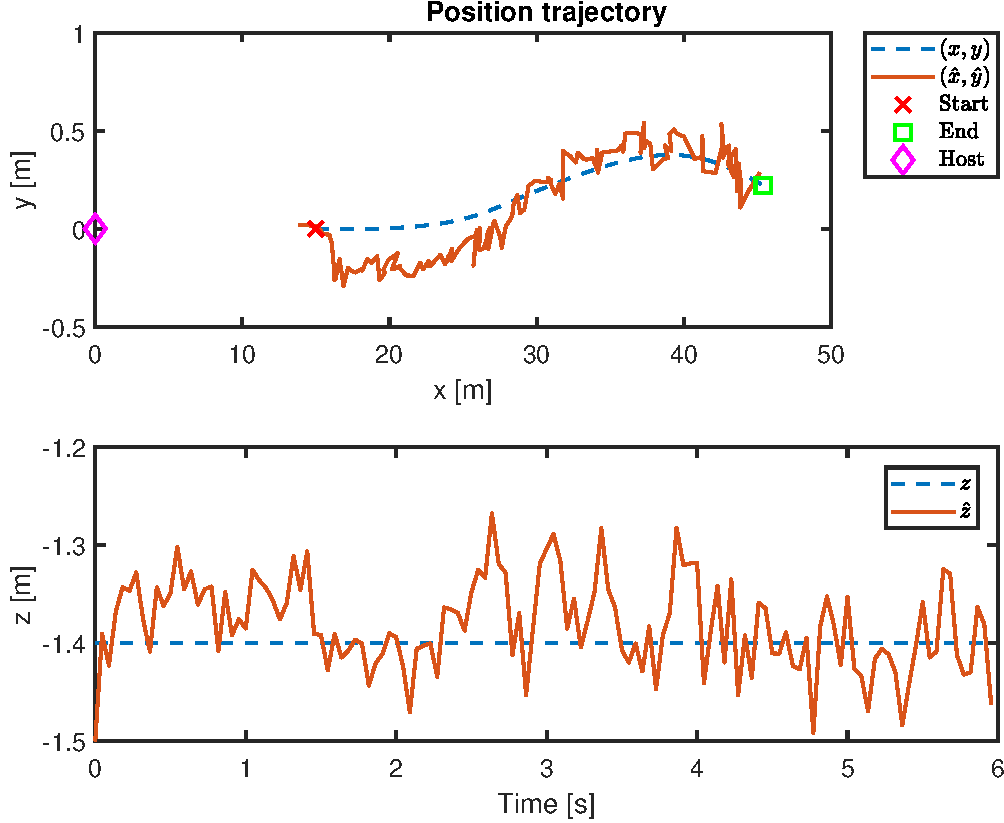
\includegraphics[width=0.8\textwidth]{ExampleTrajectory/27_MC_TrajPos}
	\caption{\label{fig:27montesimstraighttowardsroitrajpos} One example of a trajectory from the Monte Carlo simulation in scenario 1 with setup 1.}
\end{figure}

\begin{figure}[!ht]
	\centering
	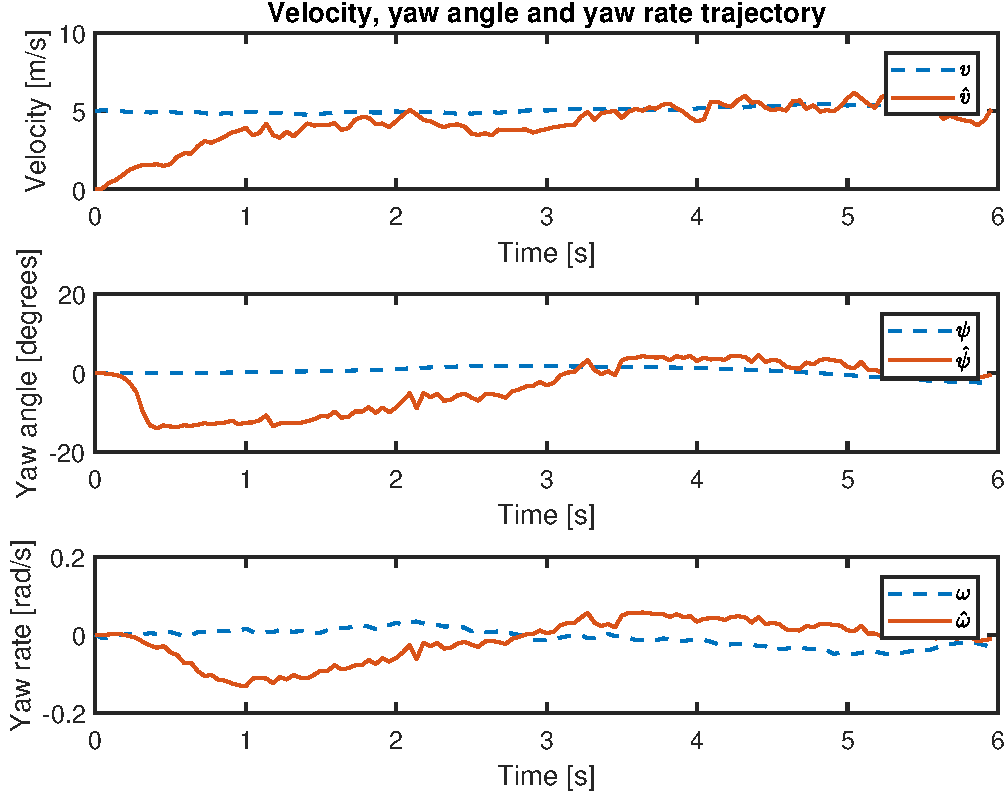
\includegraphics[width=0.8\textwidth]{ExampleTrajectory/27_MC_TrajOther}
	\caption{\label{fig:27montesimstraighttowardsroitrajother} One example of a trajectory from the Monte Carlo simulation in scenario 1 with setup 1.}
\end{figure}

\begin{figure}[!ht]
	\centering
	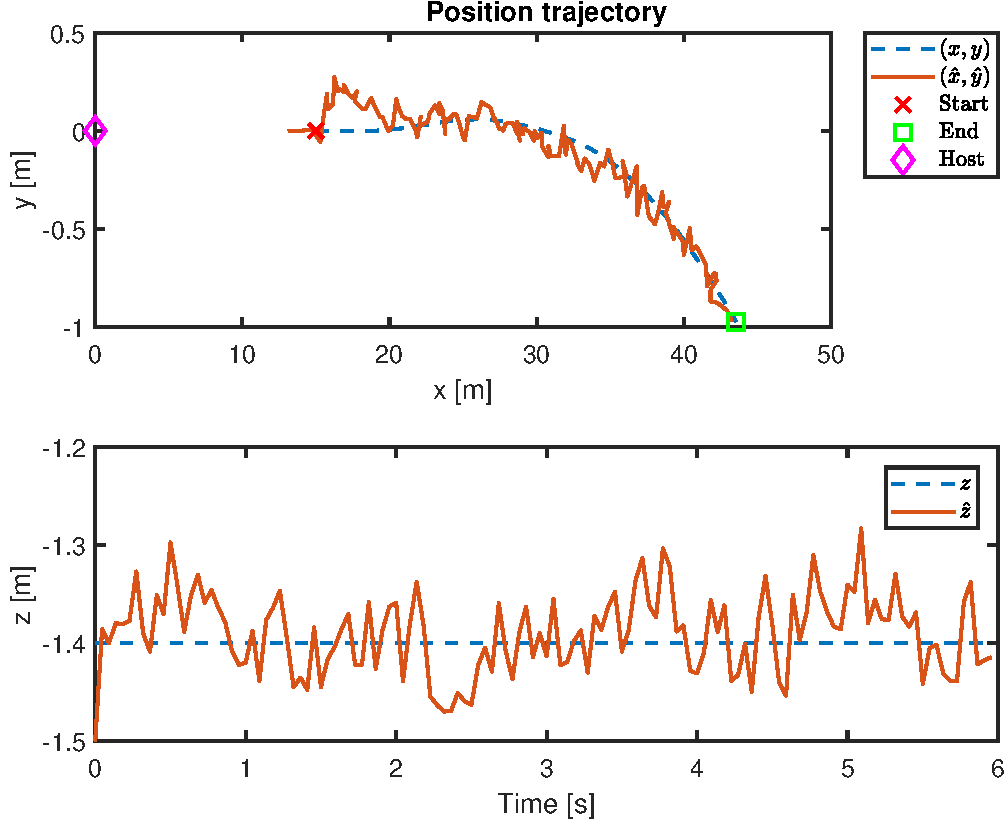
\includegraphics[width=0.8\textwidth]{ExampleTrajectory/20_MC_TrajPos}
	\caption{\label{fig:20montesimstraighttowardsroiangveltrajpos} One example of a trajectory from the Monte Carlo simulation in scenario 1 with setup 2.}
\end{figure}

\begin{figure}[!ht]
	\centering
	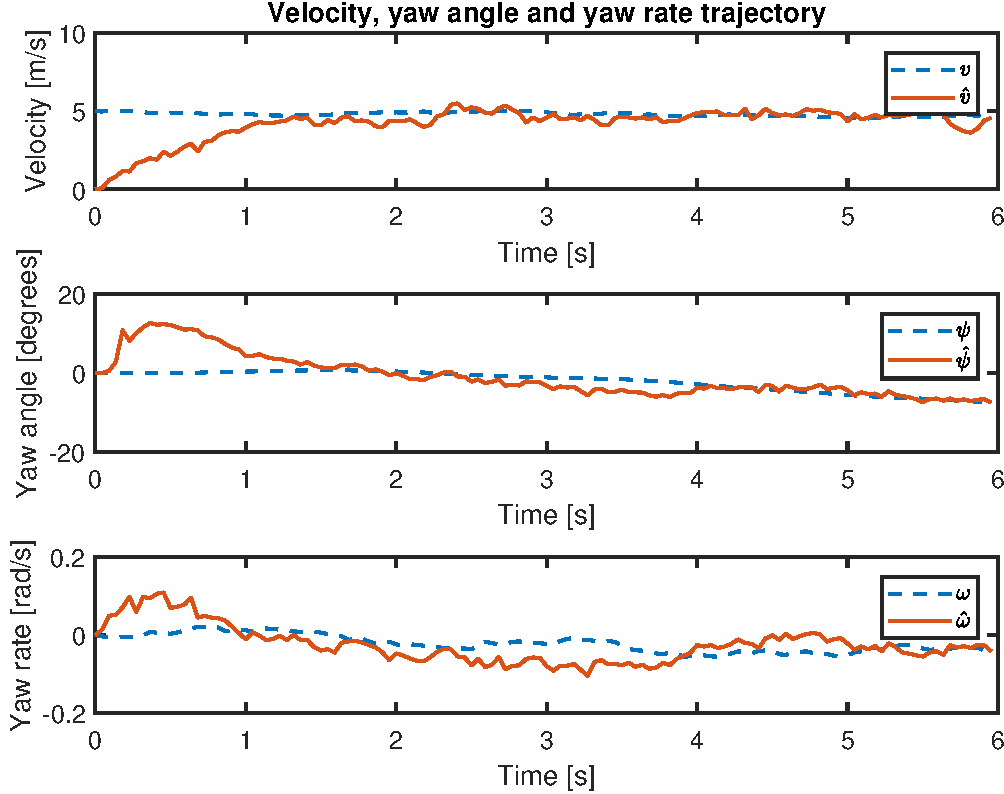
\includegraphics[width=0.8\textwidth]{ExampleTrajectory/20_MC_TrajOther}
	\caption{\label{fig:20montesimstraighttowardsroiangveltrajother} One example of a trajectory from the Monte Carlo simulation in scenario 1 with setup 2.}
\end{figure}

\begin{figure}[!ht]
	\centering
	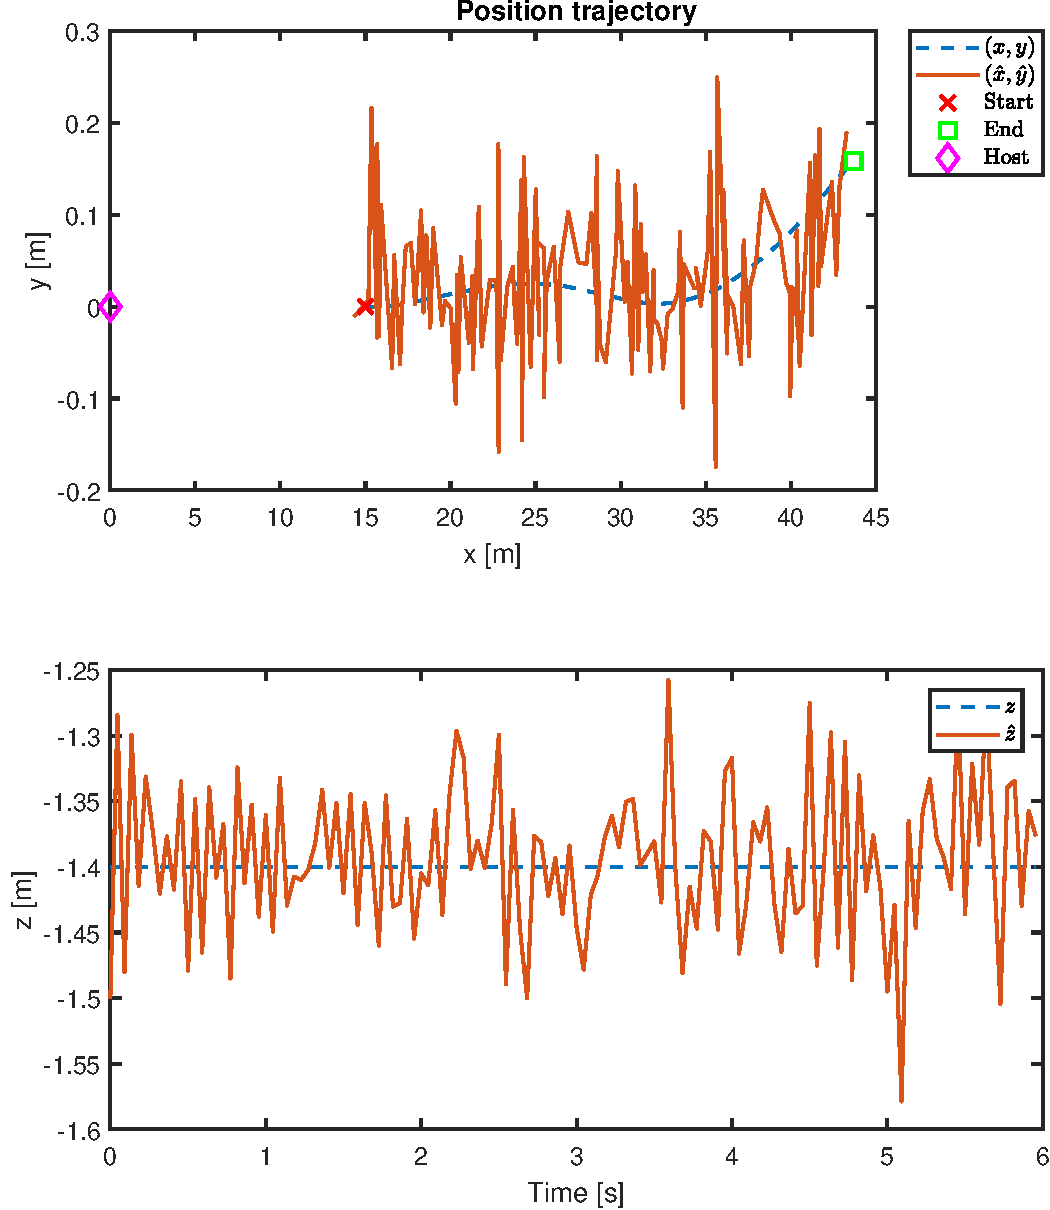
\includegraphics[width=0.6\textwidth]{ExampleTrajectory/30_MC_TrajPos}
	\caption{\label{fig:30montesimstraighttowardsroiangvelcornertrajpos} One example of a trajectory from the Monte Carlo simulation in scenario 1 with setup 5.}
\end{figure}

\begin{figure}[!ht]
	\centering
	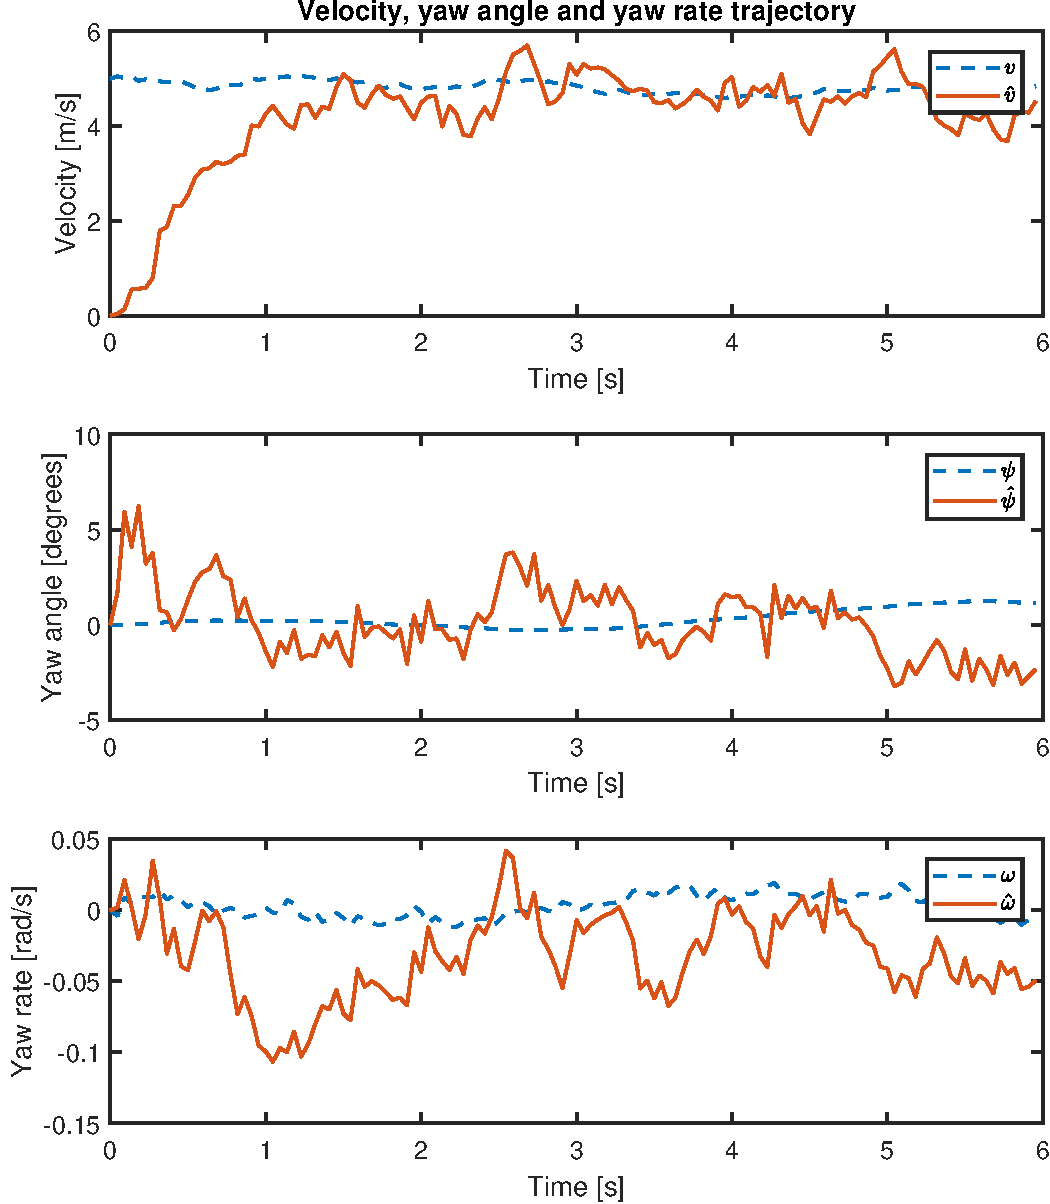
\includegraphics[width=0.5\textwidth]{ExampleTrajectory/30_MC_TrajOther}
	\caption{\label{fig:30montesimstraighttowardsroiangvelcornertrajother} One example of a trajectory from the Monte Carlo simulation in scenario 1 with setup 5.}
\end{figure}

\begin{figure}[!ht]
	\centering
	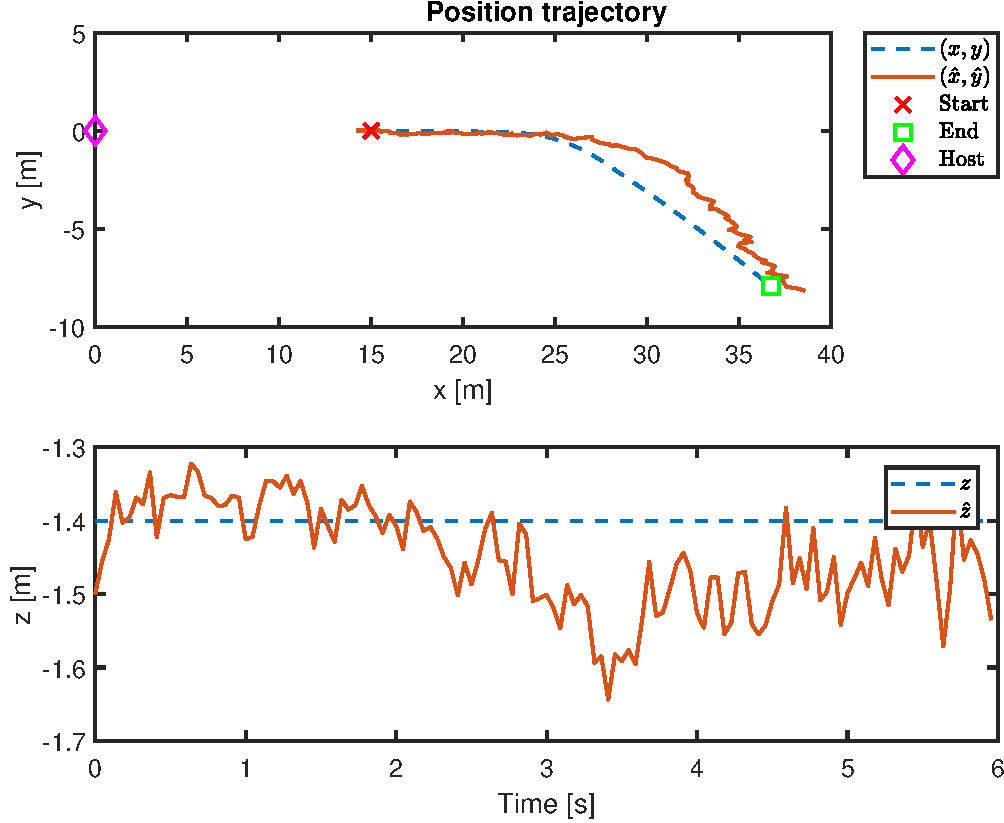
\includegraphics[width=0.8\textwidth]{ExampleTrajectory/13_MC_TrajPos}
	\caption{\label{fig:13trajectorycrossingroipos} One example of a trajectory from the Monte Carlo simulation in scenario 2 with setup 6.}
\end{figure}

\begin{figure}[!ht]
	\centering
	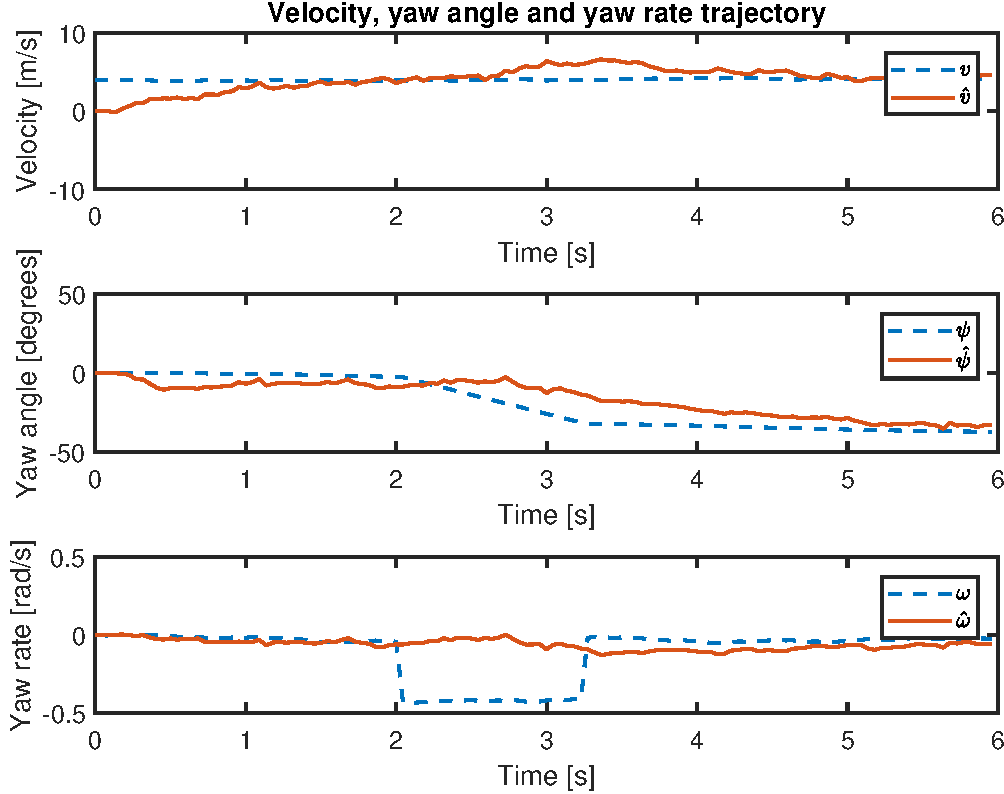
\includegraphics[width=0.8\textwidth]{ExampleTrajectory/13_MC_TrajOther}
	\caption{\label{fig:13trajectorycrossingroiother} One example of a trajectory from the Monte Carlo simulation in scenario 2 with setup 6.}
\end{figure}

\begin{figure}[!ht]
	\centering
	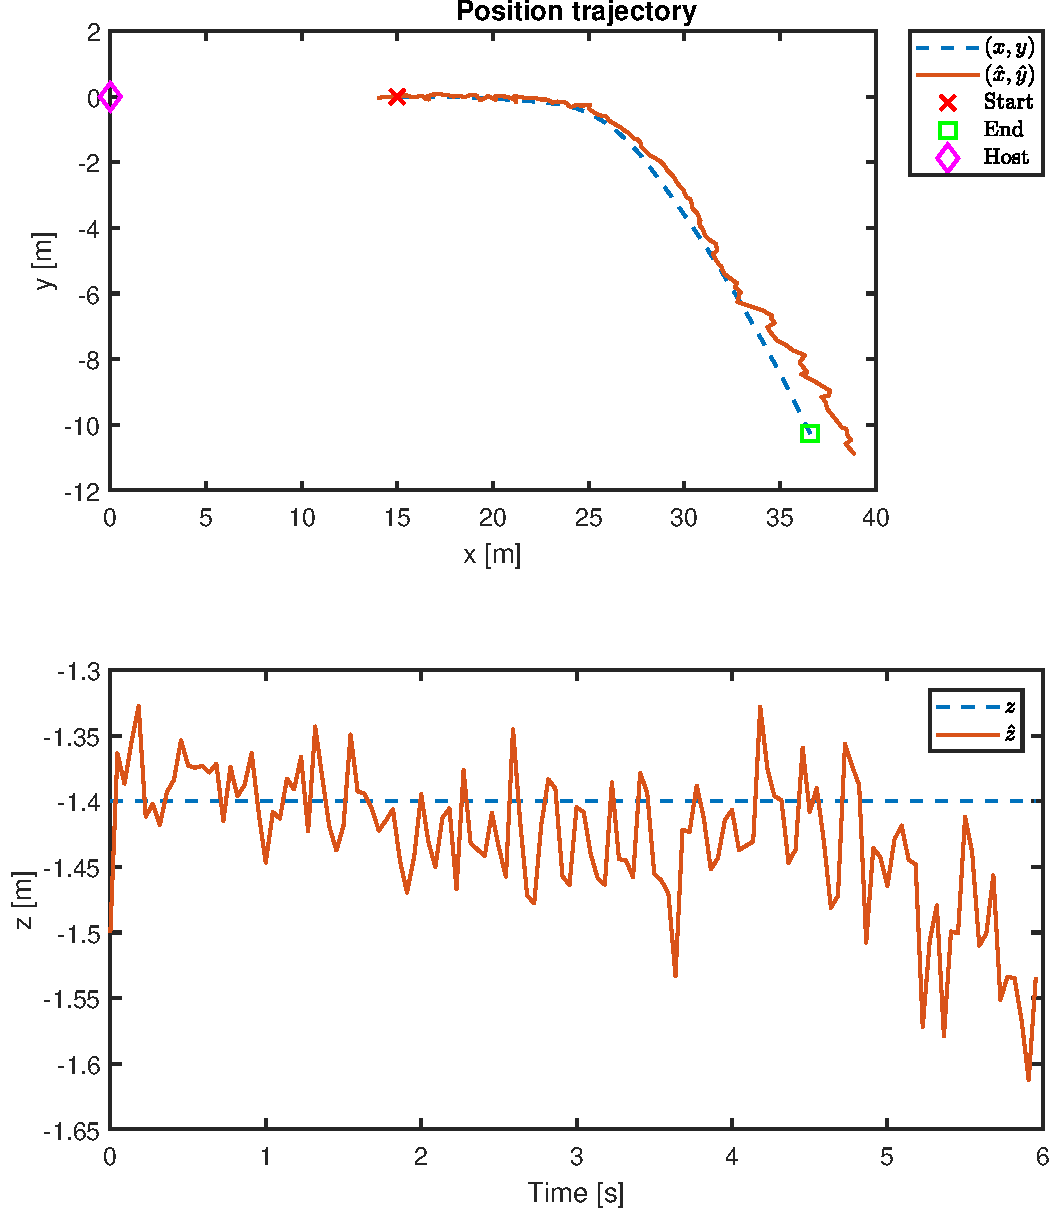
\includegraphics[width=0.6\textwidth]{ExampleTrajectory/23_MC_TrajPos}
	\caption{\label{fig:23trajectorycrossingroiangvelpos} One example of a trajectory from the Monte Carlo simulation in scenario 2 with setup 7.}
\end{figure}

\begin{figure}[!ht]
	\centering
	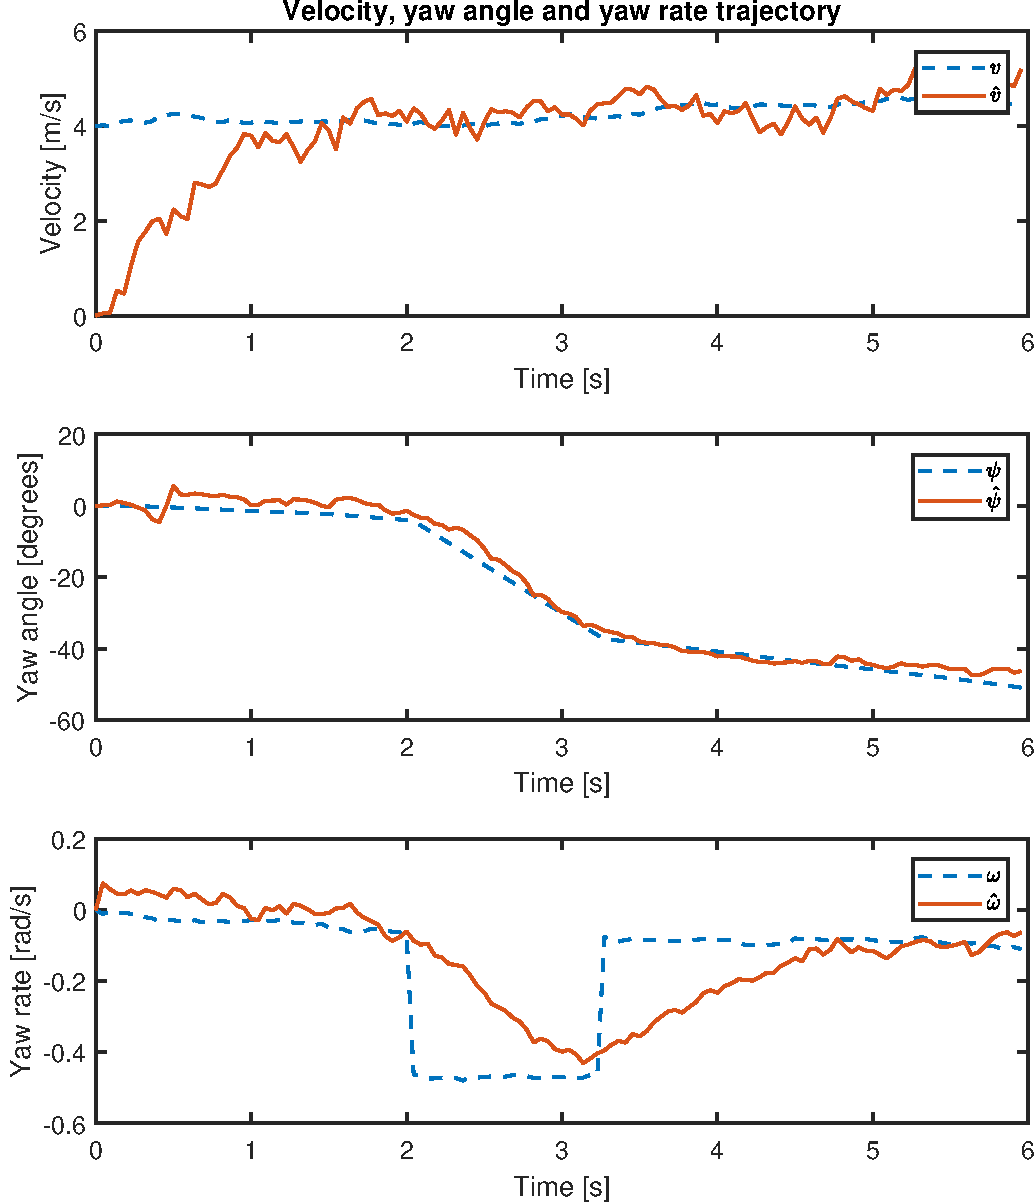
\includegraphics[width=0.5\textwidth]{ExampleTrajectory/23_MC_TrajOther}
	\caption{\label{fig:23trajectorycrossingroiangvelother} One example of a trajectory from the Monte Carlo simulation in scenario 2 with setup 7.}
\end{figure}

\begin{figure}[!ht]
	\centering
	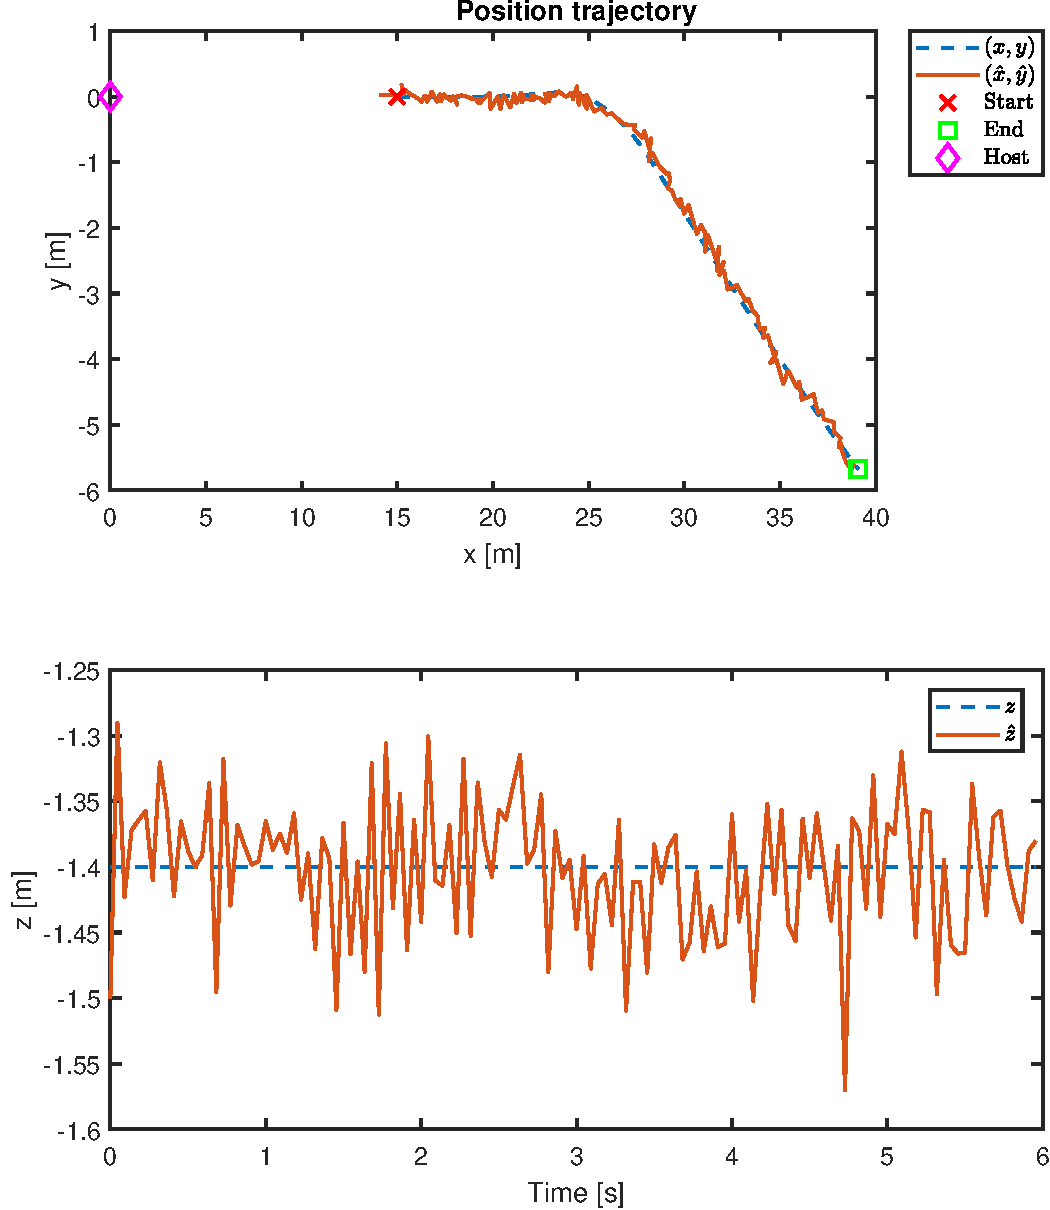
\includegraphics[width=0.6\textwidth]{ExampleTrajectory/29_MC_TrajPos}
	\caption{\label{fig:29trajectorycrossingroiangvelcornerpos} One example of a trajectory from the Monte Carlo simulation in scenario 2 with setup 10.}
\end{figure}

\begin{figure}[!ht]
	\centering
	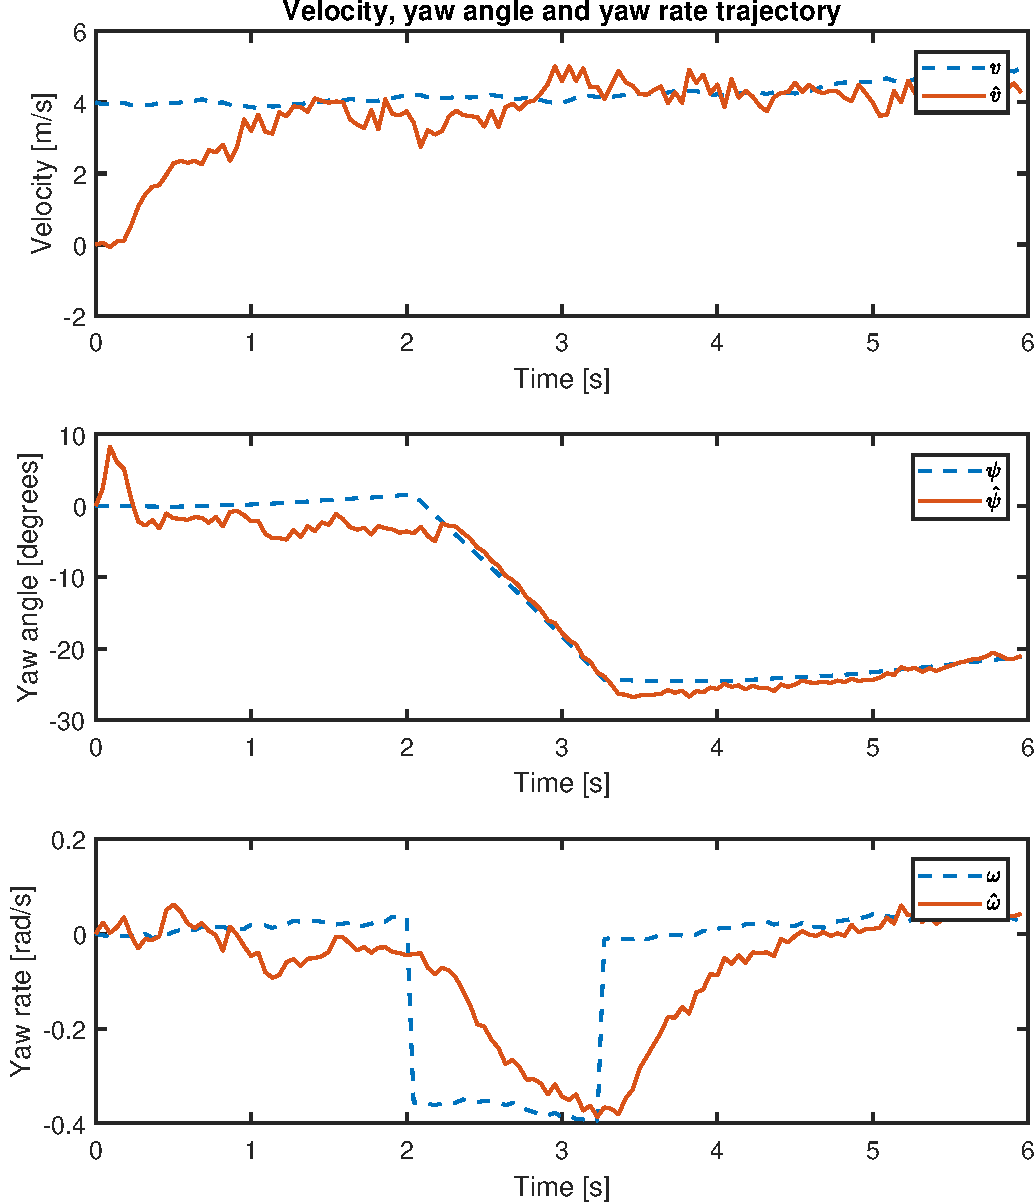
\includegraphics[width=0.5\textwidth]{ExampleTrajectory/29_MC_TrajOther}
	\caption{\label{fig:29trajectorycrossingroiangvelcornerother} One example of a trajectory from the Monte Carlo simulation in scenario 2 with setup 10.}
\end{figure}
\clearemptydoublepage
\backmatter

\bibliography{bib/IEEEfull,bib/myrefs}

\printindex

\end{document}
